\documentclass[10pt]{article}

% ---------------------------------------------------------
% MIL-STD STYLE PACKAGES
% ---------------------------------------------------------
\usepackage{geometry}
\usepackage{graphicx}
\usepackage{setspace}
\usepackage{titlesec}
\usepackage{titling}
%\usepackage{fancyhdr}
\usepackage{tocloft}
\usepackage{tabularx}
\usepackage{multirow}
\usepackage{helvet} % Sans-serif similar to MIL-STD documents
\renewcommand{\familydefault}{\sfdefault}

% Set numbering depth to include subparagraphs
\setcounter{secnumdepth}{5}

% Set Table of Contents depth to include subparagraphs
\setcounter{tocdepth}{5}

% ---------------------------------------------------------
% PAGE GEOMETRY
% ---------------------------------------------------------
\geometry{
    letterpaper,
    left=1in,
    right=1in,
    top=1in,
    bottom=1in
}

% ---------------------------------------------------------
% HEADER / FOOTER
% ---------------------------------------------------------
%\pagestyle{fancy}
%\fancyhf{}
%\lhead{MIL-STD-29A}
%\rhead{Downloaded from http://www.everyspec.com}
%\cfoot{\thepage}

% ---------------------------------------------------------
% SECTION FORMATTING
% ---------------------------------------------------------
\titleformat{\section}{\large\bfseries}{\thesection.}{1em}{}
\titleformat{\subsection}{\normalsize\bfseries}{\thesubsection}{1em}{}

% ---------------------------------------------------------
% TITLE PAGE
% ---------------------------------------------------------
\begin{document}
\begin{titlepage}
    \centering

    {\Large MIL-STD-29A \

\vspace{6pt} 1 March 1962 \par}

    \vspace{1cm}

    {\large SUPERSEDING \\ MIL-STD-29 \\ 23 September 1958 \par}

    \vfill

    {\Huge \textbf{MILITARY STANDARD} \par}
    \vspace{0.5cm}
    {\LARGE \textbf{SPRINGS, MECHANICAL;} \

\vspace{4pt}
    \textbf{DRAWING REQUIREMENTS FOR} \par}

    \vspace{1cm}

    {\Large APPENDIX OF REFERENCES TO \

\vspace{4pt}
    MATERIALS, DESIGN FORMULAS, \

\vspace{4pt}
    PROCESSES AND TOLERANCES \

\vspace{4pt}
    FOR MECHANICAL SPRINGS \par}

    \vspace{0.5cm}
    {\large (APPENDIX INCLUDES NO MANDATORY PROVISIONS) \par}

    \vfill

    {\large UNITED STATES \\ GOVERNMENT PRINTING OFFICE \\ WASHINGTON: 1962 \par}

\end{titlepage}

% ---------------------------------------------------------
% APPROVAL PAGE
% ---------------------------------------------------------
\section*{}
\begin{center}
DEPARTMENT OF DEFENSE \\
DEFENSE SUPPLY AGENCY \\
WASHINGTON 25, D.C.
\end{center}

\bigskip

\noindent
Springs, Mechanical; Drawing Requirements for \\
MIL-STD-29A \\
1 March 1962

\bigskip

\noindent
1. This standard has been approved by the Department of Defense and is mandatory
for use by the Departments of the Army, the Navy and the Air Force.

\medskip
\noindent
2. In accordance with established procedures, the Ordnance Corps, Bureau of Naval
Weapons and the Air Force, have been designated as Army-Navy-Air Force custodians
of this standard.

\medskip
\noindent
3. Recommended corrections, additions, or deletions should be addressed to the
Standardization Division, Defense Supply Agency, Washington 25, D.C.

\newpage

% ---------------------------------------------------------
% CONTENTS PAGE
% ---------------------------------------------------------
%\section*{CONTENTS}
%\addcontentsline{toc}{section}{CONTENTS}

\section{Scope}
\subsection{Scope}
This standard illustrates the approved method of drawing, dimensioning, and specifying spring data on detail drawings of each type of mechanical spring described herein.
Adherence to this standard is mandatory in the preparation of drawings prepared by or for the Department of Defense.
Appendix A contains material, design and manufacturing data representative of modern spring engnieering.
It is included herein for guidance and conveniance only and contains no mandatory provisions.

\subsubsection{Types of Springs}

The types of springs describeed in this standard are:
\paragraph{Compression}
(a) Helical, Cylindrical; (b) Helical, Stranded Wire; (c) Volute; (d) Coned Disc (Belleville)
\paragraph{Extension}
(a) Helical
\paragraph{Torsion}
(a) Helical; (b) Volute; (c) Spiral
\paragraph{Flat}
(a) Cantilever
\paragraph{Constant Force}
(a) Flat Strip
\paragraph{Garter}
(a) Helical

\subsection{Purpose}
The purpose of this standard is to establish uniform methods of specifying end product data for mechanical springs on drawings prepared by or for the Department of Defense.

\section{Referenced Documents}
\subsection{Not Applicable}

\section{Definitions}
\subsection{Mechanical Spring}
An elastic body whose mechanical function is to store energy when deflected under load and return the equivalent amount of energy upon being released.
\subsection{Load}
The force exerted upon or by a spring in order to reproduce or modify motion or to maintain a force system in equilibrium.
A static load is slowly applied and does not subject a spring to fatigue.
A dynamic load is either a suddenly applied load or one that causes impact due to kinetic energy. 
It also may be frequently repeated, thus shortening fatigue life.
\subsection{Total Deflection}
The movement of a spring from free position to its maximum operating position. 
In a compression spring, it is the deflection from the Free
Length to the Solid Length.
\subsection{Deflection per Coil}
The total deflection of the spring divided by the number of active coils.
\subsection{Set}
The permanent distortion from the manufactured dimensions which occurs when the spring is stressed beyond the elastic limit of the material.
\subsection{Active Coils}
The number of coils which are used in computing the total deflection of the spring.
\subsection{Total Coils}
The number of active coils plus the coils forming the ends, (Compression Springs).
\subsection{Solid Length}
The overall length of a compression spring when all coils are fully compressed.
\subsection{Free Length}
The overall length of a spring in the unloaded position.
\subsection{Pitch}
The distance between centers of adjacent active coils of a spring in the unloaded position.
\subsection{Initial Tension}
A load wound into certain helical extension springs during the
coiling operation which keeps the coils tightly closed and which must be exceeded by an appleid load before the coils begin to open.
\subsection{Spring Index}
The ratio of the mean spring diameter to the diameter of the wire.
\subsection{Spring Rate}
The load required to deflect a commpression or extension spring one inch or the load required to deflect a torsion spring one degree or one revolution. 
Also referred to as "Scale," "Gradient" and "Load Factor."
\subsection{Torque}
A turning force about an axis multiplied by the distance from the
load to the axis, usually expressed in pound-inches (LB IN.) or in ounce-inches (OZ IN.) and always used in conjunction with the number of degrees of rotation, number of revolutions or deflected position.
\subsection{Spring Tolerance}
The permissible variations from a given dimension.
\subsection{Factor of Safety}
The ratio of the maximum load a spring can sustain without permanent set to the maximum applied load.
\subsection{Direction of Helix}
When a spring is viewed from one end, the direction of helix is right hand when the coil recedes in a clockwise direction, and left hand when it recedes in a counterclockwise direction. 
A right hand helix follows the same direction as the threads on a standard screw. 
A left hand helix is most popular for compression and extension springs.
\subsection{Reference Dimension}
A reference dimension is a dimension without tolerance which is entered on a drawing for informational purposes and which does not directly govern manufacturing or inspection operations. 
Reference dimensions are indicated on drawings by writing the abbreviation REF directly following or under the dimension.
\subsection{Stress Relieve}
To subject springs to a low temperature heat treatment after coiling or bending to remove residual stresses caused by the forming operation. 
Also called "strain relieve", "stress equalizing", "tempering", "blueing" and "baking".
\subsection{Range of Stress}
The difference between the stress at maximum and minimum loads.
\subsection{Harden}
To cause a material to become harder by heat treatment. 
Spring steels are heated above the critical temperature and quenched in oil. 
Precipitation hardening alloys such as Beryllium-Copper, K-Monel and Inconel X are heated at elevated temperatures for extended periods of time.
\subsection{Endurance Limit}
The maximum stress range of stress at which a material will operate indefinitely without failure. 
This limit for springs is usually determined at 10,000,000 cycles of deflection.
\subsection{Elastic Limit}
The maximum stress to which a material may be subjected without causing a permanent set. 
Also the stress beyond which a material must be subjected to form a coil, radius or bend.
\subsection{Modulus of Rigidity}
The measure of elastic ability. 
A mathematical constant expressing the stiffness, rigidity, elasticity and flexibility of a material. 
Also called "modulus of elasticity" and "Young modulus".

\section{General Requirements}
\subsection{Not Applicable}

\section{Detail Requirements}

\subsection{General}
Figures 2(a) through 2(d), 4(a) through 4(d), 7, 10, 12, 13, 14, 16, 17 and 18 are Drawing Requirement Charts illustrating approved methods of drawing and dimensioning the various types of springs listed in paragraph 1.1.1 and include compilations of spring data to be used as applicable when prescribing manufacturing information on detail drawings of mechanical springs. 
The inclusion herein of these charts should not be interpreted as restricting the scope of spring characteristics to be specified on engineering drawings delineating springs. 
The specification of correct and complete manufacturing data is the responsibility of the cognizant Design Activity.
Figures 19 thru 30 are examples of typical detail drawings of springs illustrating the application of the information included on the charts.

\subsubsection{Delineation}
The simplified drafting methods shown on the Drawing Requirement Charts and the typical detail drawings, e.g., Figures 2(a) and 19, are generally satisfactory for depicting helical springs.

\subsection{Specifications Applicable to All Springs}

\subsubsection{Material Specifications}
Material specifications are designated in the space provided in the title block on the drawing. 
When such space is inadequate enter therein "SEE NOTE" and describe the material requirments in a general note.

\subsubsection{Diameter of Wire}
Wire diameter, or width an thickness of material, shall be designated in decimals, or common fractions of an inch, as applicable, and unless otherwise specified, all dimensions apply before plating or applying finishes. 
Such dimensions are used to avoid confusion resulting from various gage numbering systems in current use. 
However, they should conform with the appropriate gage customarily used with the material specified, whenever possible. 
For oil tempered and corrosion resisting steels such diameters should conform with the U. S. Steel Wire Gage, which is the same as the Washburn \& Moen Gage. 
For non-ferrous materials the American Wire Gage, which is the same as the Brown \& Sharpe Gage, is used. 
Music Wire is drawn to the American Steel Wire and Music Wire Gage but other gages and intermediate sizes are available. 
Do not specify the name of the Gage used. 
Tolerances on diameter and thickness shall not be specified when they are covered in the appropriate material specifications or by general tolerance notes.
Specify a tolerance on the width, as applicable. 
See Table I, Preferred Sizes of Spring Materials, in Appendix A, Section I.

\subsubsection{Inspection Notes}
Detail drawings of springs that are critical, including those
springs subjected to critical conditions of temperature, stress or corrosive environments, shall include appropriate instruction
notes applicable to controlling the manufacture within the desired environments. 
It is appropriate to specify those spring factors requiring inspection, the tests required, and whether all springs produced from the particular drawing shall be inspected. 
Consistent with Quality Control Procedure the size of inspection samples shall not be specified.

\subsection{Format for Special Data Notes}
When notes prescribing special data are required on detail drawings of springs, it is recommended that the following format be used:

(a) Stress at ... F +/- ... F for ... minutes, after coiling (or forming)

(b) Hardness range Rc ... to ...

(c) Squareness of ends in free position within ... degrees

(d) Cold set to solid.

(e) Shot peen (give specification) to ... intensity.

(f) Protective coating (give specification).

(g) Non destructive inspection (give specification).

(h) The body shall not camber more than ... IN. in its entire length

(i) Test over arbor dia ... IN.

(j) To withstand temperatures of ... F for ... hours with loss of load not to exceed ... \%.

(k) To withstand ... deflections from initial to final position with loss of load not to exceed ... \%.

\subsection{Helical Compression Springs}

\subsubsection{Definition}
A compression spring is an open-coil helical spring that offers resistance to a compressive force applied axially. 
Compression springs are generally made cylindrical in form, although other forms are used, such as conical, tapered, concave or convex, consistent with design requirements. 
Because of ready supply, wire of circular cross section is used whenever possible; however, where advantageous to design, wire of
square or rectangular cross section may be utilized. 
Figure 1 illustrates several forms of helical compression springs.

\subsubsection{Drawing Requirements}
Guide lines for specifying pertinent dimensional and load data on engineering drawings of helical compression springs, which satisfy specific design requirements and, simultaneously, allow maximum latitude in manufacturing, are provided herein, categorized as follows:

(1) No Load Specified. 

The design activity assumes responsibility for the load capacity of the spring. 
The manufacturer is required to furnish a spring meeting the dimensional data specified. 
The free length, the coil diameter, and the total number of coils are specified, each with a tolerance.
The tolerance on the wire diameter conforms to the governing material specification.
Figure 2(a) shows suggested data applicable to springs in the "no load" category.

(2) One Load Specified.

This category has application when the spring is required to develop a load, within a specified tolerance, preferably at the initial assembled length.
The spring, normally, is not subjected to further deflection in operation. 
The manufacturer is required to meet the load requirement, but the free length and the total number of coils are not restricted, being designated REF. 
The tolerance on the wire diameter conforms to the governing material specification and the manner of coil diameter callout is dependent upon spring function. 
Figure 2(b) shows suggested data applicable to springs in the "one load" category.

(3) Two Loads Specified. 

This category has application when the spring is required to develop a load within a specified tolerance, at each of two definite compressed lengths, normally at the initial and the final operating positions in the assembly. 
The manufacturer is required to meet the load requirements, other spring characteristics being designated as described in paragraph 5.4.2 (2). 
Figure 2(c) shows suggested data applicable to springs in the "two loads" category.

(4) Spring Rate Specified. 

This category has application in assemblies in which the spring rate is the most significant characteristic, for example, in calibrated scales. 
The manufacturer is required to meet a prescribed spring rate, within a specified tolerance, but the free length and the total number of coils are permitted to vary, being designated REF. 
The tolerance on the wire diameter conforms to the governing material specification and the manner of coil diameter callout is dependent upon the spring function. 
Additionally, when closer control of the load to be developed at the initial assembled length is desired, one load, with a tolerance, to be developed at the assembled length should be specified. 
Figure 2(d) shows suggested data applicable to springs in the "spring rate" category.

\paragraph{Coil Diameter}
Depending upon the application of the spring, specify one of the
following:

(a) TO WORK OVER...IN. (MAX) DIA ROD

(b) TO WORK IN...IN. (MIN) DIA BORE

(c) ID, with tolerance

(d) OD, with tolerance
\paragraph{Direction of Helix}
When governed by design requirements, specify the direction of helix as "LEFT HAND" (or LH), or "RIGHT HAND" (or RH), as applicable; otherwise specify as OPTIONAL. 
In most cases the hand is not important except when a plug screws into an end; or when one spring fits inside another, in which case one spring should be designated left hand and the other right hand.
\paragraph{Type of Ends}
The types of ends having application to helical compression springs are illustrated in Figure 3. 
Specify the type of ends on the drawing; when necessary, the ends should be dimensioned.
\paragraph{Solid Length}
The maximum solid length shall be specified for any spring category when this parameter is essential to design requirements. 
However, solid length callout should be omitted whenever practicable. 
Except when necessary to satisfy function, springs should not be designed to go solid in operation.

\clearpage

\begin{figure}[htbp] % h:here, t:top, b:bottom, p:page
    \centering
    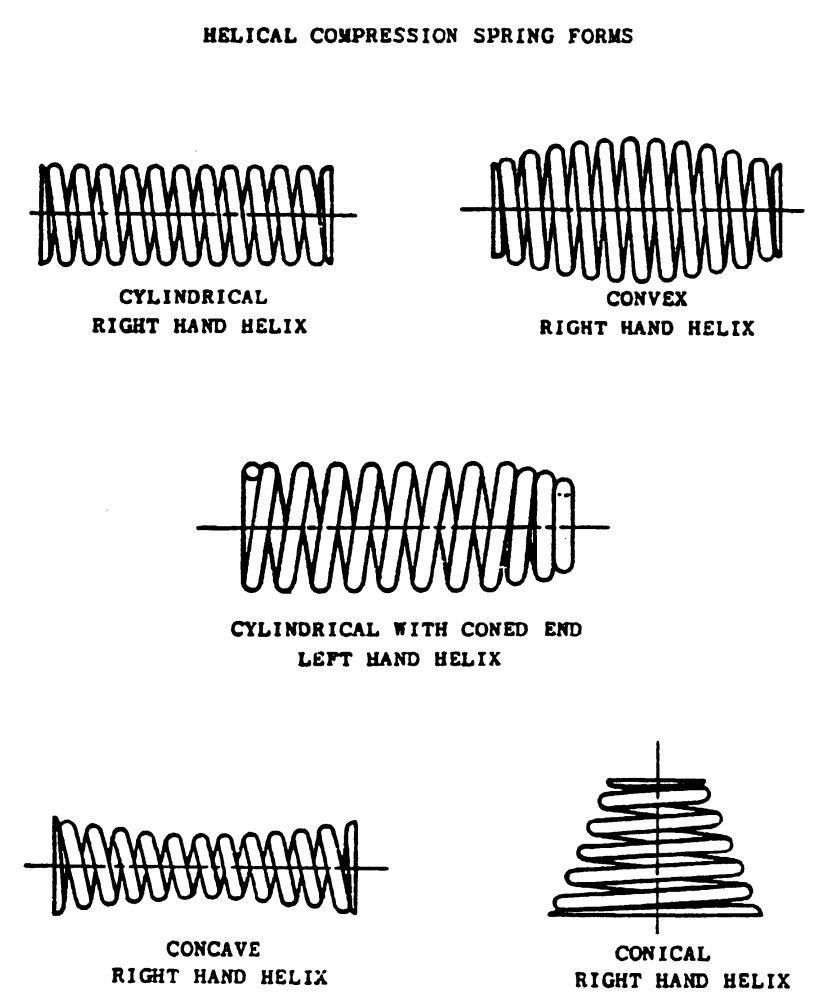
\includegraphics[width=0.8\textwidth]{milstd29a_fig1.png}
    \caption{Helical Compression Spring Forms}
    \label{fig:1}
\end{figure}

\begin{figure}[htbp] % h:here, t:top, b:bottom, p:page
    \centering
    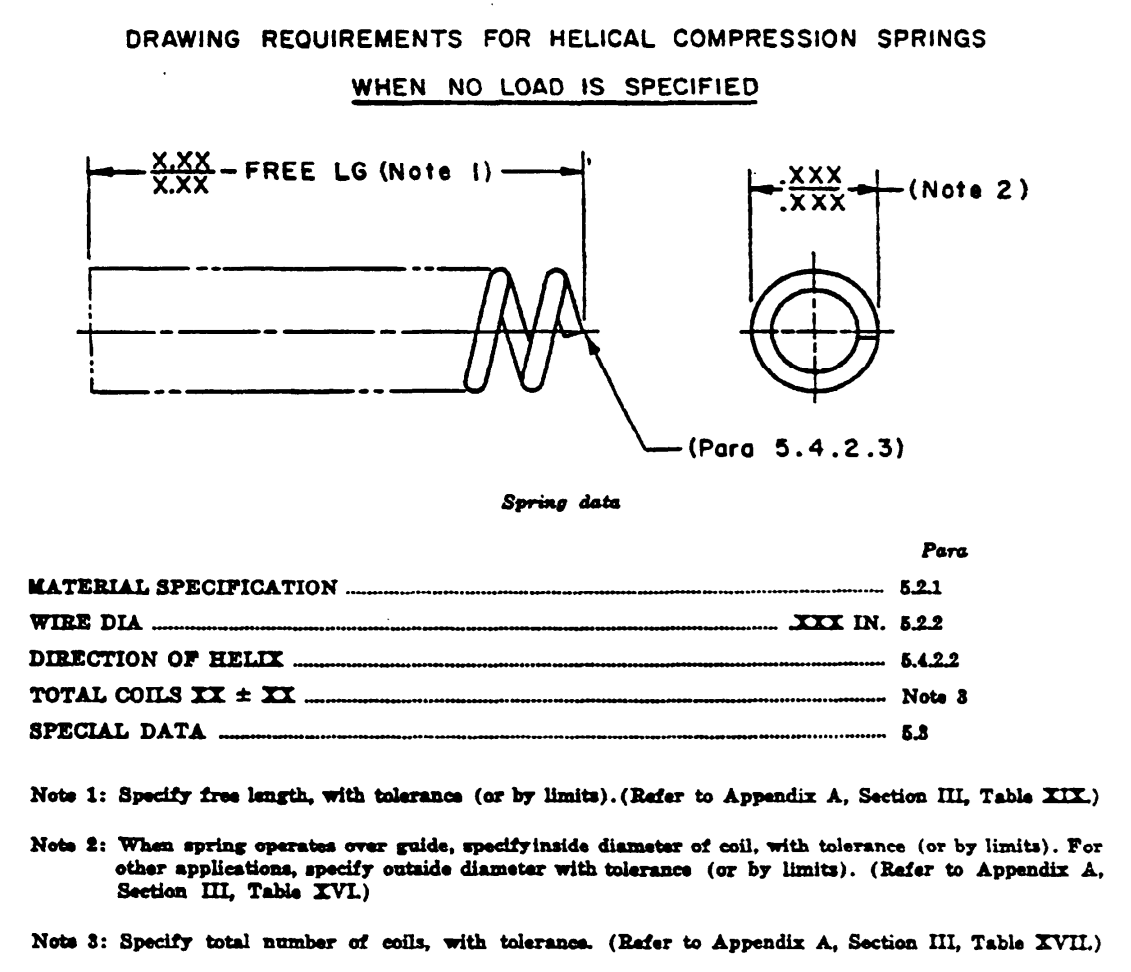
\includegraphics[width=0.8\textwidth]{milstd29a_fig2a.png}
    \caption{}
    \label{fig:2a}
\end{figure}

\begin{figure}[htbp] % h:here, t:top, b:bottom, p:page
    \centering
    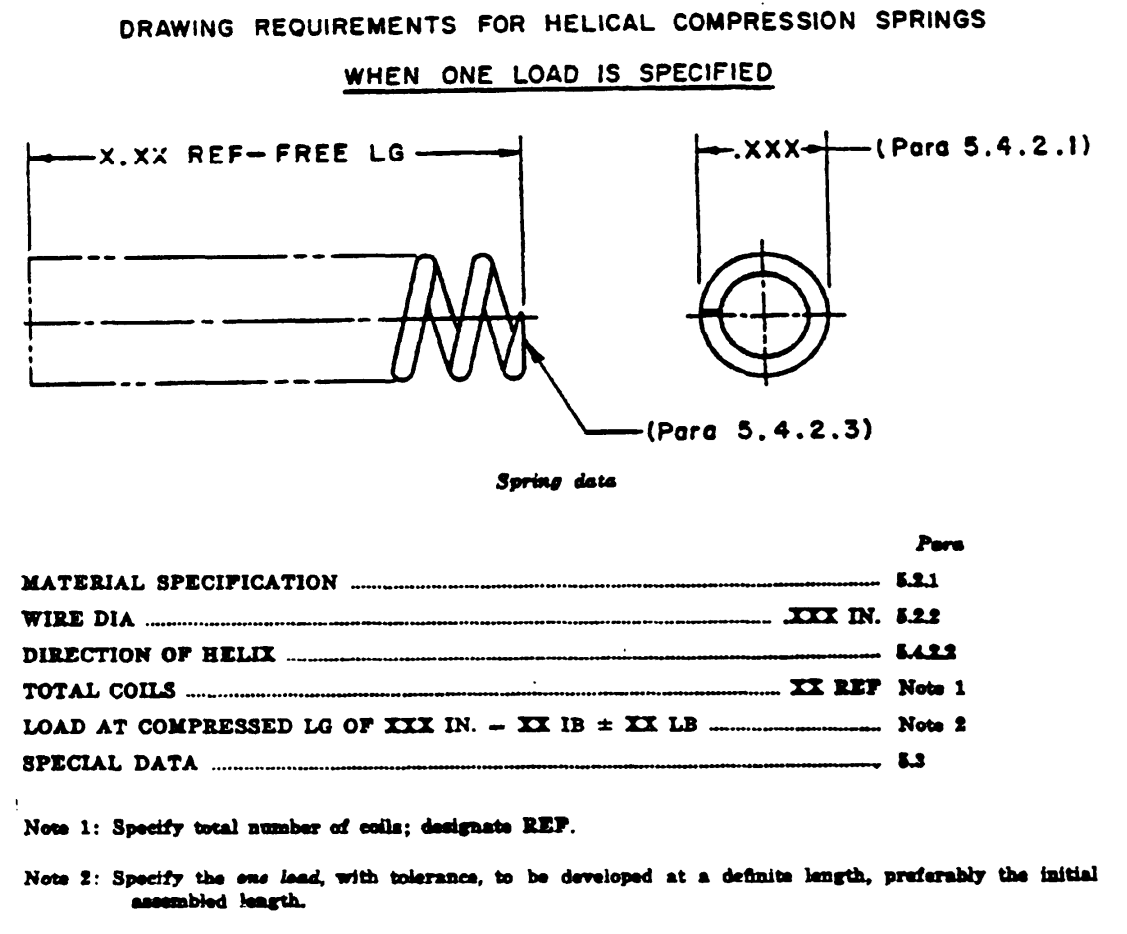
\includegraphics[width=0.8\textwidth]{milstd29a_fig2b.png}
    \caption{}
    \label{fig:2b}
\end{figure}

\begin{figure}[htbp] % h:here, t:top, b:bottom, p:page
    \centering
    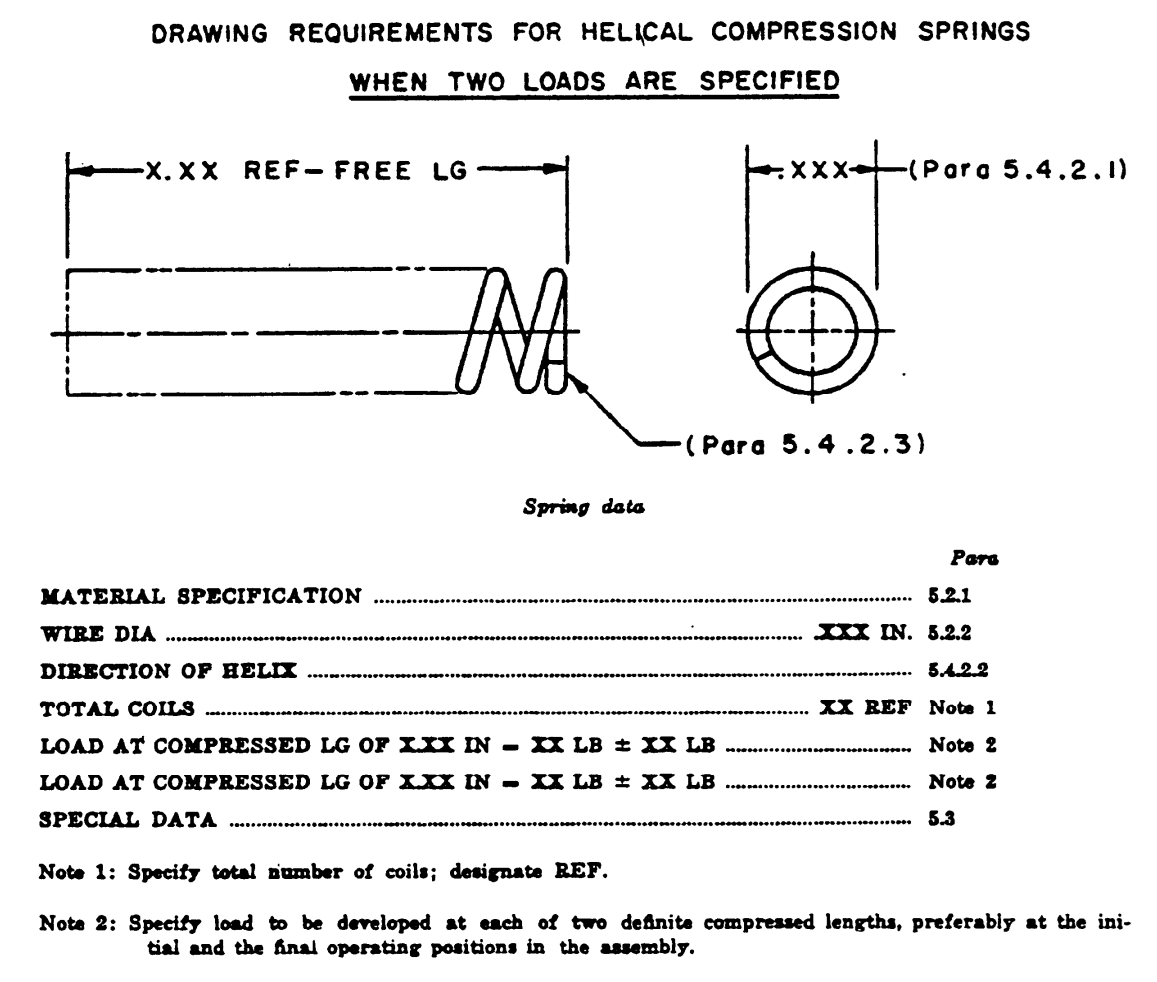
\includegraphics[width=0.8\textwidth]{milstd29a_fig2c.png}
    \caption{}
    \label{fig:2c}
\end{figure}

\begin{figure}[htbp] % h:here, t:top, b:bottom, p:page
    \centering
    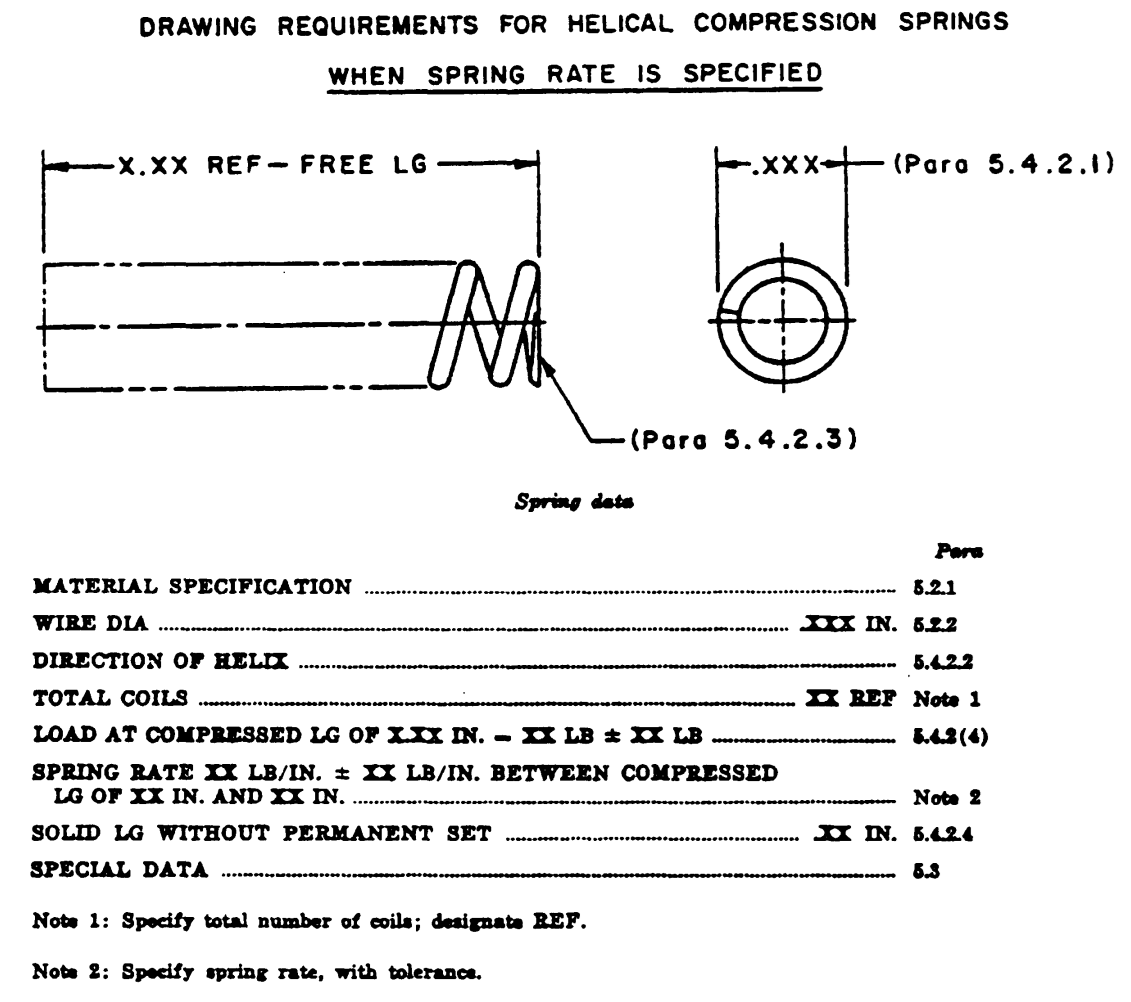
\includegraphics[width=0.8\textwidth]{milstd29a_fig2d.png}
    \caption{}
    \label{fig:2d}
\end{figure}

\clearpage

\subsection{Stranded Wire Compression Springs}
\subsubsection{Definition}
Stranded wire compression springs are helical compression springs formed from two, three, or more wires twisted about each other, or about one wire as a core, to form a single strand. 
Stranded wire compression springs have the advantage of damping the migratory waves that traverse the spring under shock loading. 
Such springs should be specified with caution since stranded wire is specially made and is not readily available.

\subsubsection{Drawing Requirements}
Figure 20 is a typical detail drawing of a stranded wire helical compression spring. 
The methods of drawing and dimensioning, and the spring data applicable to stranded wire spring correspond in general to those shown in Figures 2(c) for compression springs, except that the additional spring information noted herein is required on detail drawings:

(a) Number of Wires in Strand.

(b) Diameter of each Wire.

(c) Length of Lay (Distance parallel to strand axis in which a single wire makes one turn.)

(d) Direction of strand helix. NOTE: The strand helix shall be opposite in turn to the coil helix.

(e) Direction of coil helix (Left Hand or Right Hand).

(f) Type os Ends. Specify either Closed Ends Not Ground or Open Ends Not Ground, as applicable. 
Specify that ends are to be soldered, brazed, or welded to prevent unraveling, and sharp burrs shall be removed.

\subsection{Helical Extension Springs} % Section 5.6
\subsubsection{Definition}  % Section 5.6.1
A helical extension spring is a close-wound spring with or without initial tension, or an open-wound spring that offers resistance to an axial force tending to extend its length. 
Extension springs are formed or fitted with ends which are used for attaching the spring to the assembly. 
They are generally made of wire of circular cross-section, but when advantageous to design, may be made of wire of square or rectangular cross-section.
Extension springs may be wound with adjacent coils touching so lightly that deflection begins the instant a load is applied. However, they are usually designed to retain abut 10\% of their maximum applied load as initial tension. 
This holds the coils together thus making it easier to coil the springa and meet test requirements. 
They may also be wound so tightly, that a large portion of the applied load (up to about 33\% of the maximum load) must be expended before actual deflection occurs. 
Figure 5 illustrates various forms of helical extension springs.

\subsubsection{Drawing Requirements for Helical Extension Springs}  % Section 5.6.2
Guidelines for specifying dimensional and load data on engineering drawings showing helical extension springs
are similar to those established for helical compression springs. 
Figures 4(a) through 4(d) show suggested guidelines for use, selectively, in delineating helical extension springs, in the categories described in paragraph 5.4.2.

\paragraph{Total Coils and Length Over Coils}  % Section 5.6.2.1
All coils in an extension spring usually are active.
Exceptions are those with plug ends and those with end coils coned over swivel hooks. 
Specify the total number of coils and the length over coils each as REF, except as noted in Figure 4(a).

\paragraph{Maximum Extended Length}  % Section 5.6.2.2
Specify the maximum allowable extended length without permanent set as a protection against over extending the spring during assembly only if essential to design requirements.
Be sure the total stress at this deflection is less than the elastic limit in torsion.

\paragraph{Types of Ends}  % Section 5.6.2.3
Typical types of ends applicable to helical extension springs are illustrated in Figure 6. 
The types of ends required shall be completely delineated and dimensioned on the drawing. 
Usually the outside diameter of a hook or loop is the same as the outside diameter of the spring.
A "Hook" has an open space between its end and the body of the spring. 
A "Loop" is a closed hook.

\paragraph{Relative Position of Ends}  % Section 5.6.2.4
When controlled by assembly requirements, the relative position of the ends shall be specified with a tolerance; otherwise include in the spring data this note:

RELATIVE POSITION OF ENDS UNIMPORTANT

\begin{figure}[htbp] % h:here, t:top, b:bottom, p:page
    \centering
    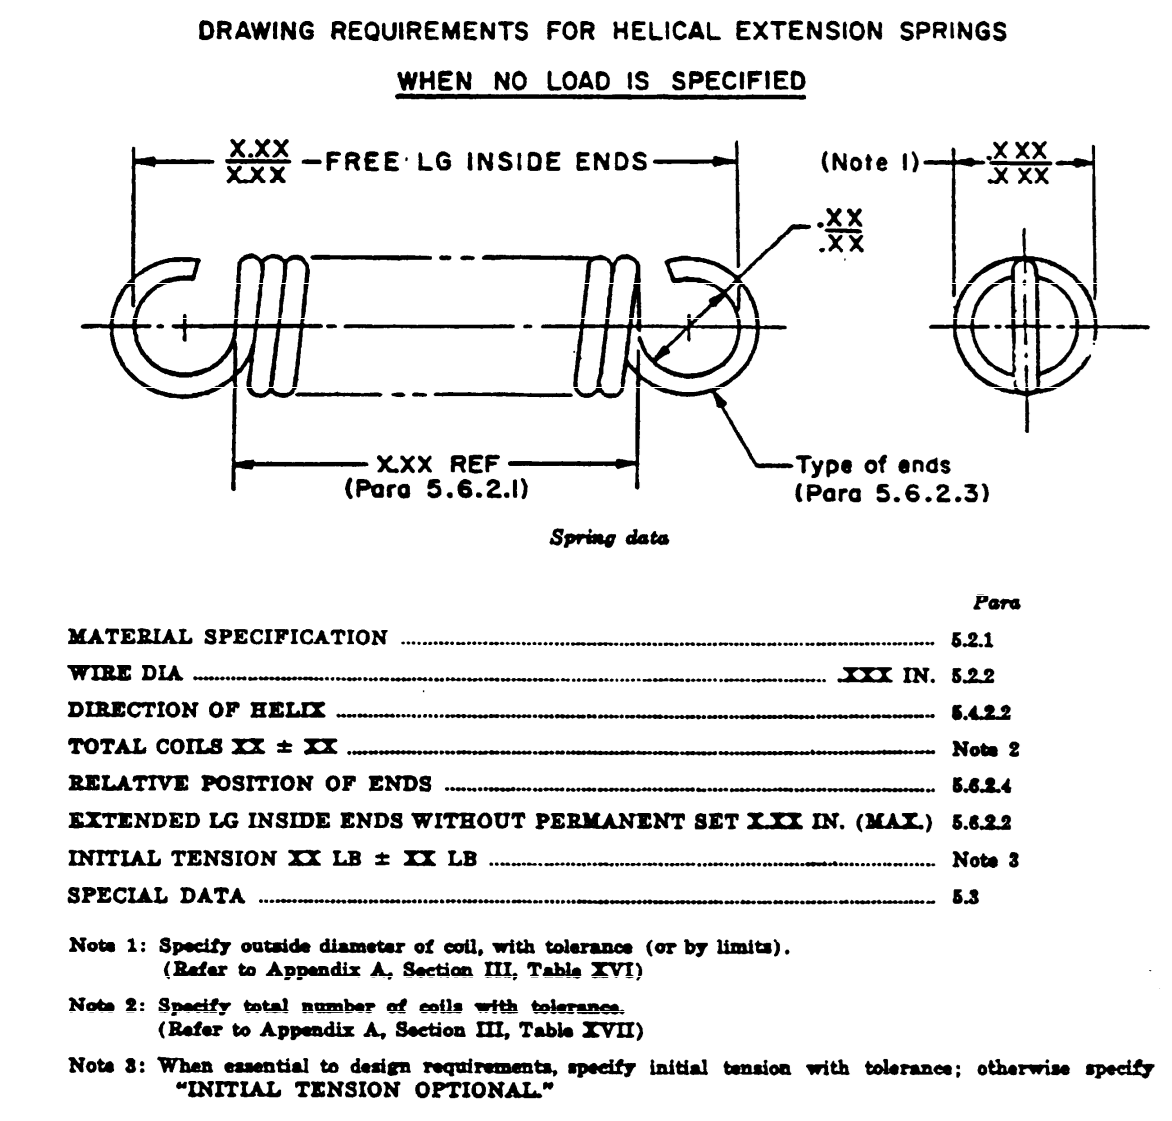
\includegraphics[width=0.8\textwidth]{milstd29a_fig4a.png}
    \caption{}
    \label{fig:2d}
\end{figure}

\begin{figure}[htbp] % h:here, t:top, b:bottom, p:page
    \centering
    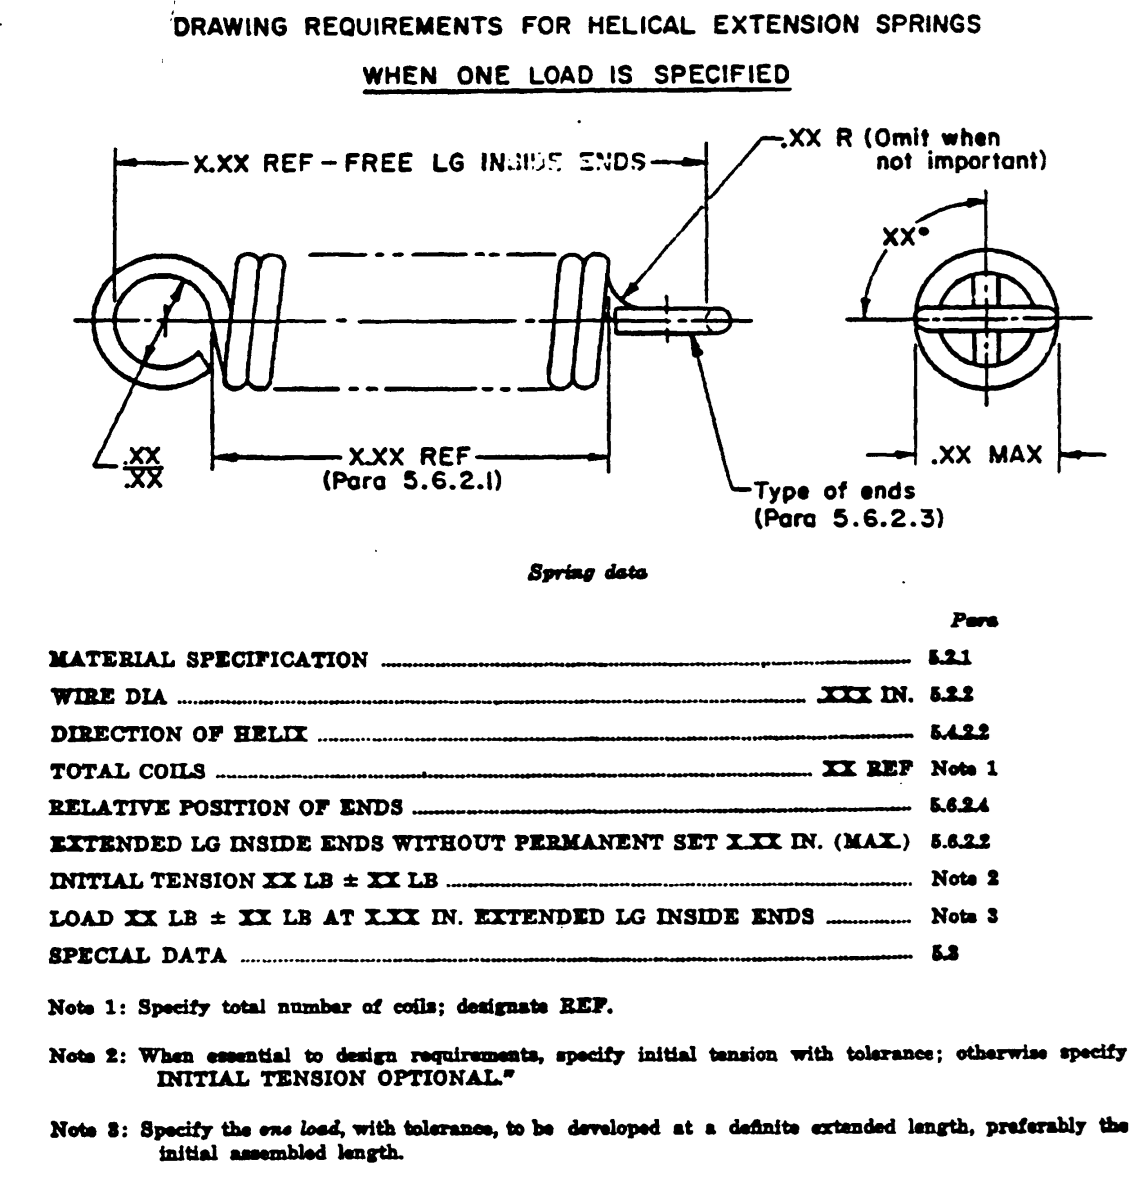
\includegraphics[width=0.8\textwidth]{milstd29a_fig4b.png}
    \caption{}
    \label{fig:2d}
\end{figure}

\begin{figure}[htbp] % h:here, t:top, b:bottom, p:page
    \centering
    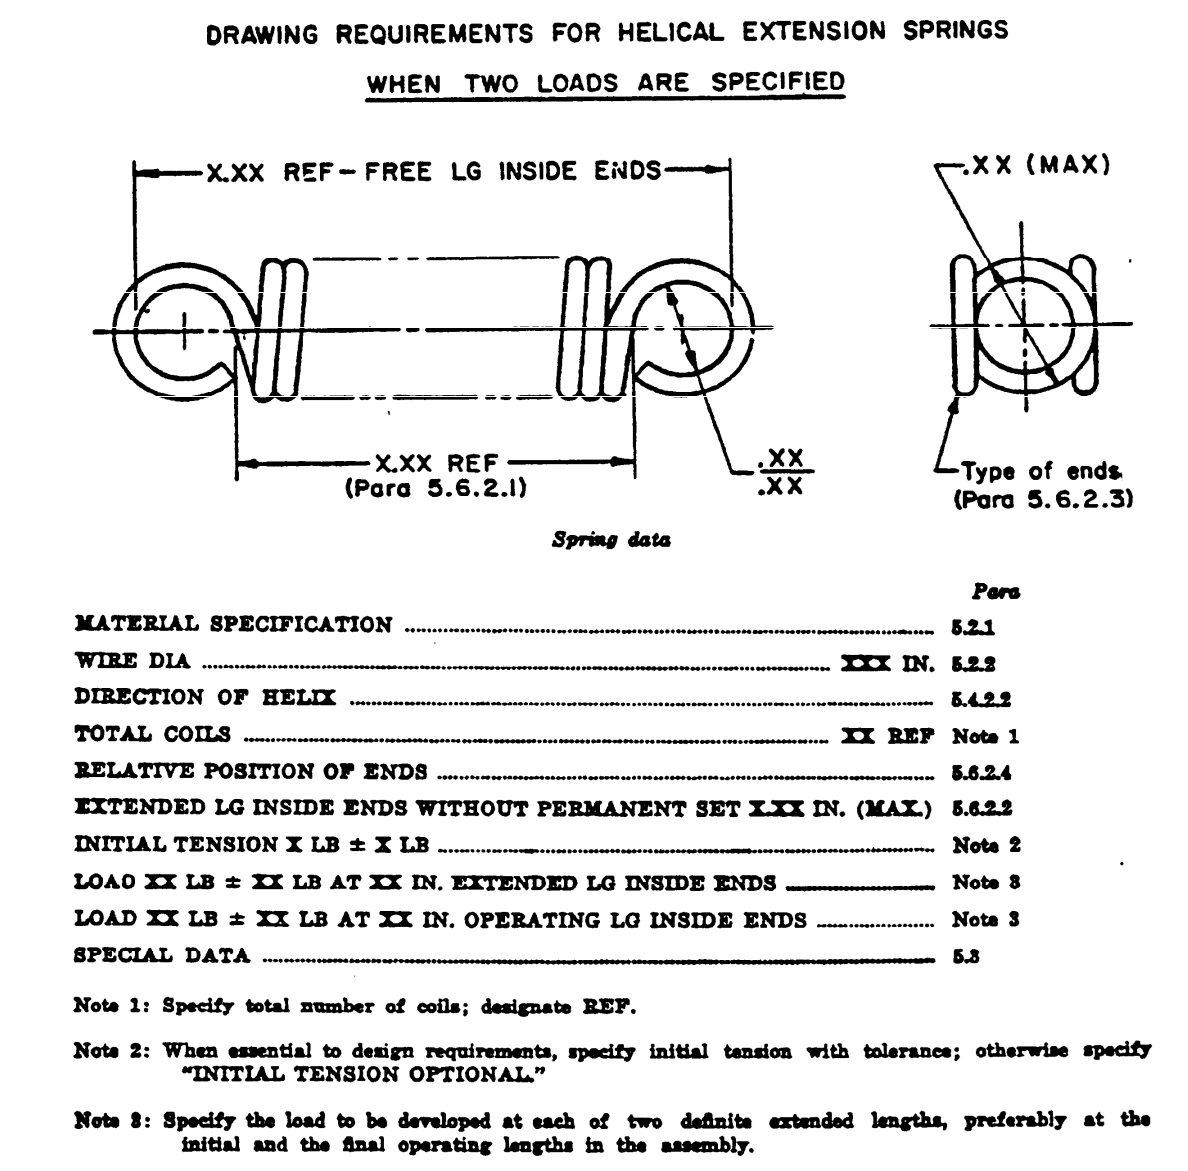
\includegraphics[width=0.8\textwidth]{milstd29a_fig4c.png}
    \caption{}
    \label{fig:2d}
\end{figure}

\begin{figure}[htbp] % h:here, t:top, b:bottom, p:page
    \centering
    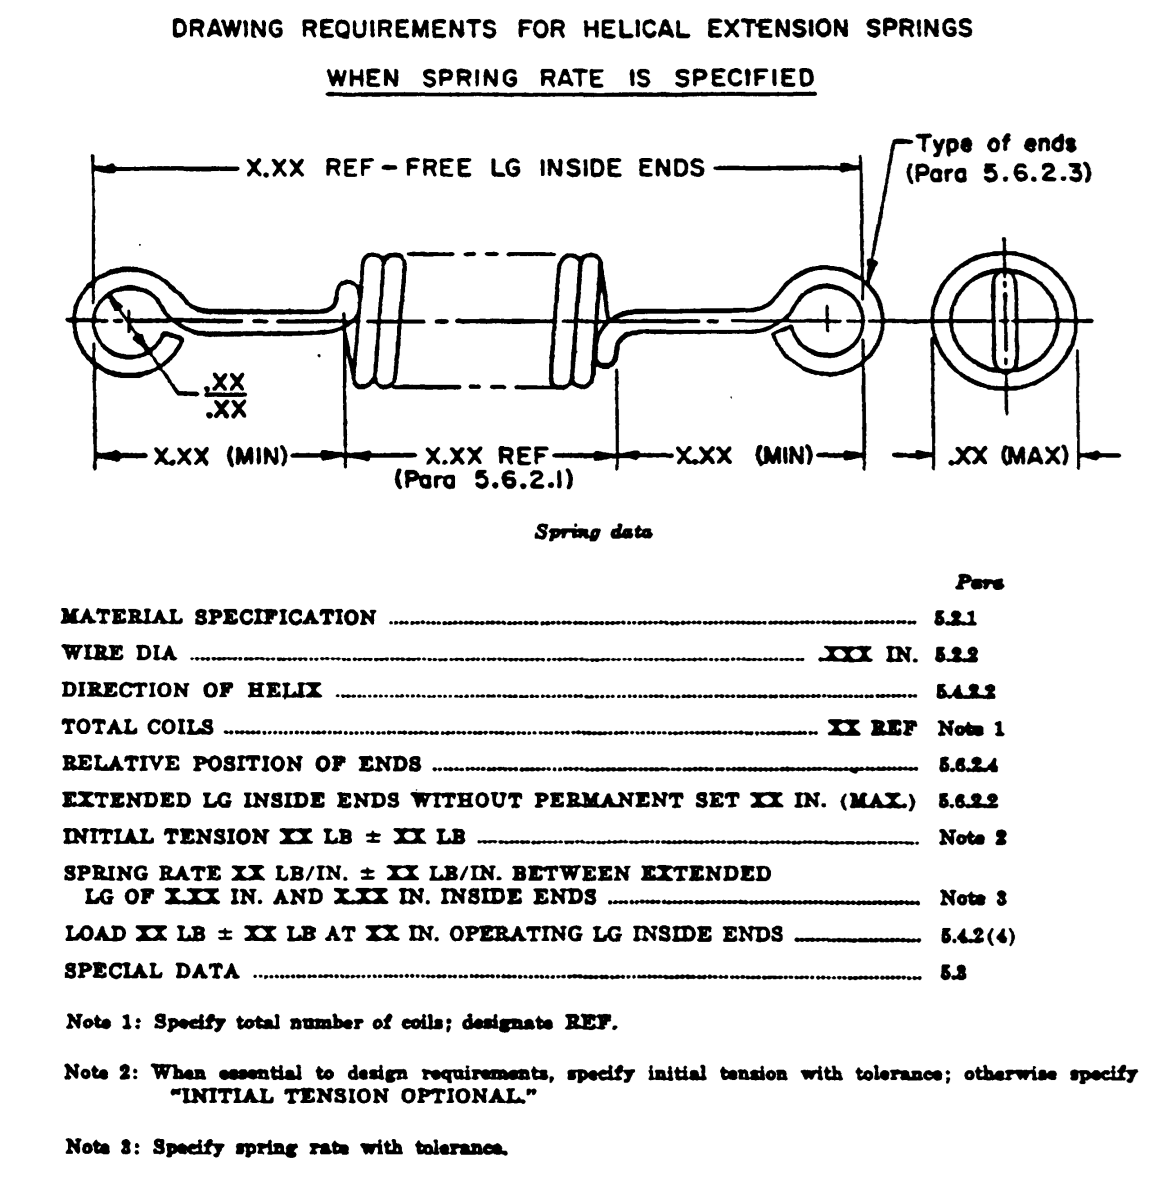
\includegraphics[width=0.8\textwidth]{milstd29a_fig4d.png}
    \caption{}
    \label{fig:2d}
\end{figure}

\begin{figure}[htbp] % h:here, t:top, b:bottom, p:page
    \centering
    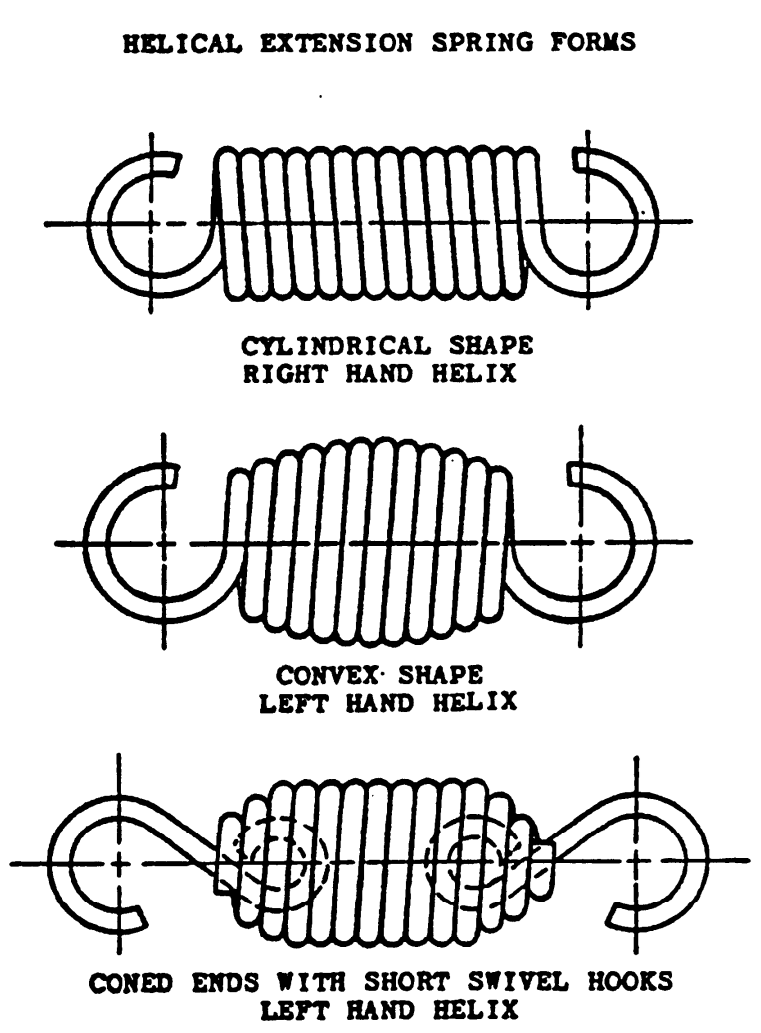
\includegraphics[width=0.8\textwidth]{milstd29a_fig5.png}
    \caption{}
    \label{fig:2d}
\end{figure}

\begin{figure}[htbp] % h:here, t:top, b:bottom, p:page
    \centering
    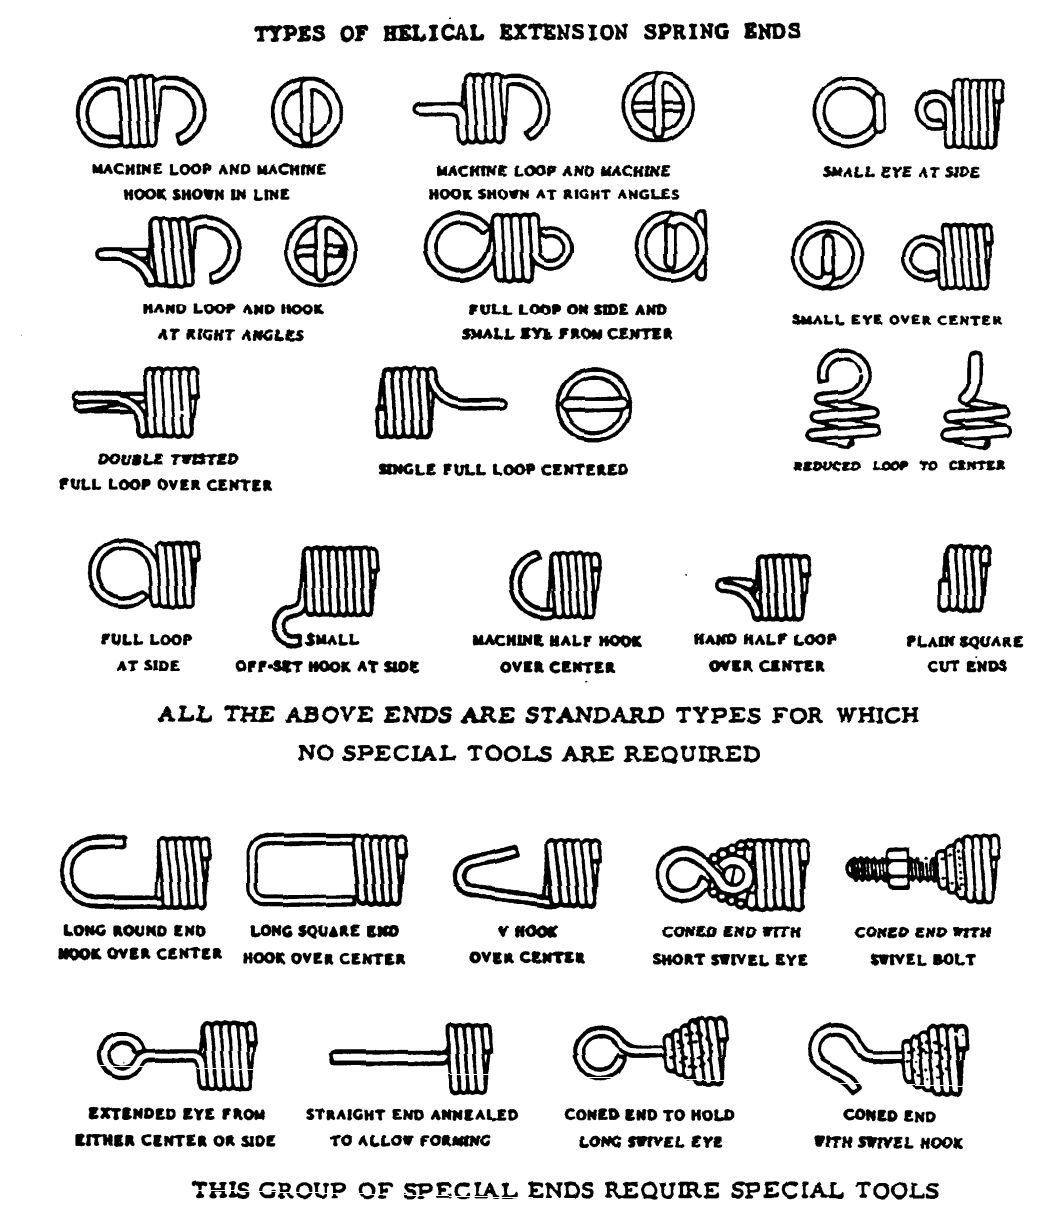
\includegraphics[width=0.8\textwidth]{milstd29a_fig6.png}
    \caption{}
    \label{fig:2d}
\end{figure}

% pg 19:
\clearpage
\subsection{Helical Torsion Springs}  % Section 5.7
\subsubsection{Definition} % Section 5.7.1
Helical torsion springs are springs that offer resistance to or exert a turning force in a plane at right angles to the axis of the coil. 
Torsion springs are generally made of circular cross section in a variety of forms and are employed in applications seldom alike. 
Figures 8 and 9 illustrate various forms of torsion springs and some of the ends used on such springs.

\subsubsection{Drawing Requirements for Helical Torsion Springs} % Section 5.7.2
Explanation of the spring data listed in Figure 7 is given below. 
Figure 22 is a typical drawing of a torsion spring.

\paragraph{Total Coils and Length Over Coils} % Section 5.7.2.1
All coils in a torsion spring usually are active.
Specify the total number of coils and the length over coils in the free position each as REF, or with tolerances, if essential to the design.

\paragraph{Direction of Helix} % Section 5.7.2.2
(yet to be transcribed)

\paragraph{Pitch of Coils or Initial Tension} % Section 5.7.2.3
(yet to be transcribed)

\paragraph{Torque Loads} % Section 5.7.2.4
Specify the torque loads at the initial and final positions between the deflected end and not at deflection from free position. 
However, if more than one revolution is required, specify the number of revolutions from the free position.
Example: 40 lb in. +/- 4 lb in. at 2.5 revolutions from free position. 
Tolerances shaIl be applied to the torque loads but not to the angle betxveen the ends. 
Also state under SPECIAL DATA the diameter of the arbor or rod over which the spring is tested, which should be the same size as the shaft over which it is operated.

\paragraph{Maximum Deflection without Permanent Set}
(yet to be transcribed)

\paragraph{Spring Rate}
Specify the spring rate in pound inches per degree of deflection as a REFERENCE except where particular design requirements necessitate a tolerance.
Examples of such applications are in calibrated scales or instruments. 
When the spring rate is specified with a tolerance designate the loads at deflected positions as a REFERENCE.

\paragraph{Type of Ends}
Some of the types of ends applicable to helical torsion springs are illustrated in Figures 8 and 9. 
The types of ends required and the relative position of the ends shall be completely dimensioned and clearly delineated on the drawing.

\begin{figure}[htbp] % h:here, t:top, b:bottom, p:page
    \centering
    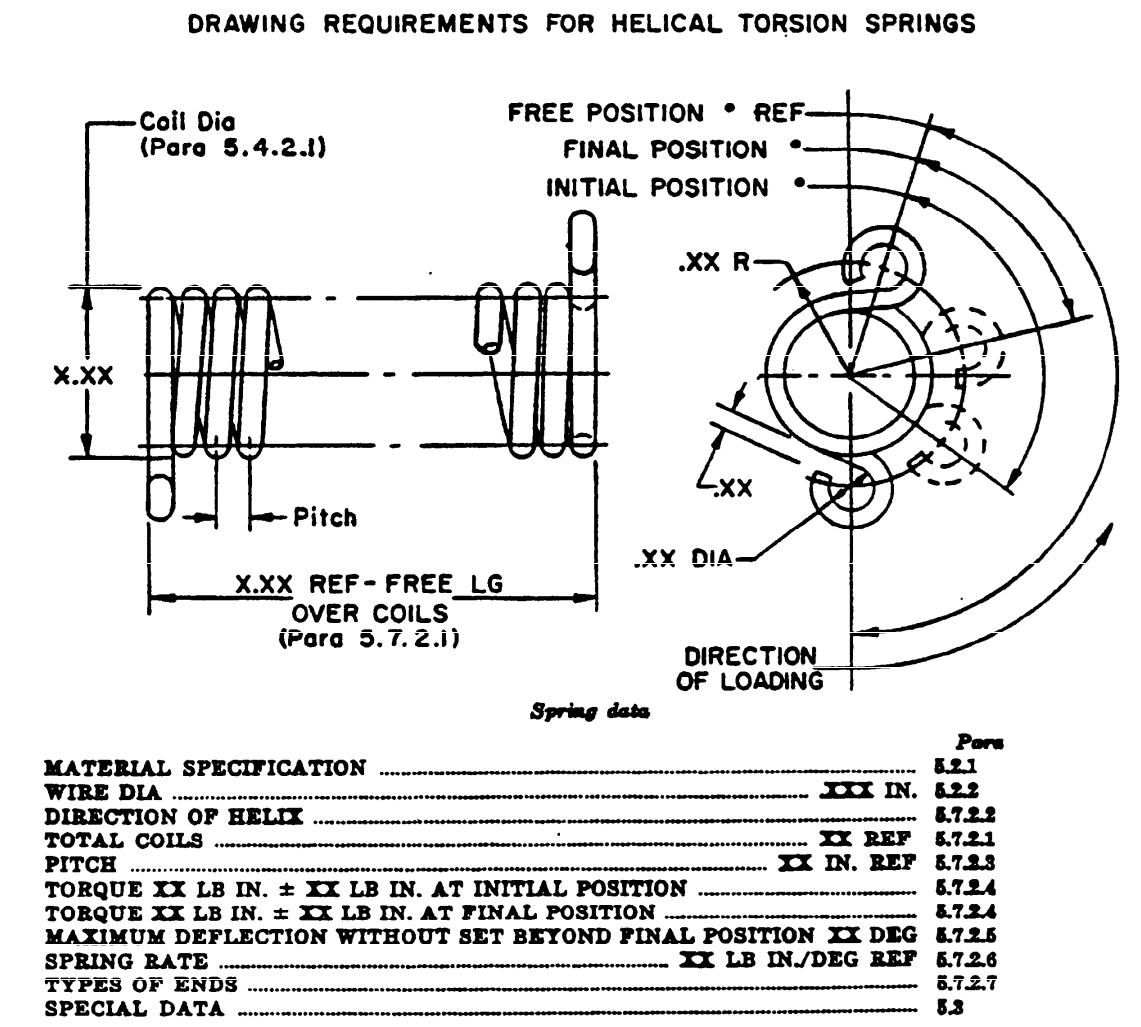
\includegraphics[width=0.8\textwidth]{milstd29a_fig7.png}
    \caption{}
    \label{fig:2d}
\end{figure}

\begin{figure}[htbp] % h:here, t:top, b:bottom, p:page
    \centering
    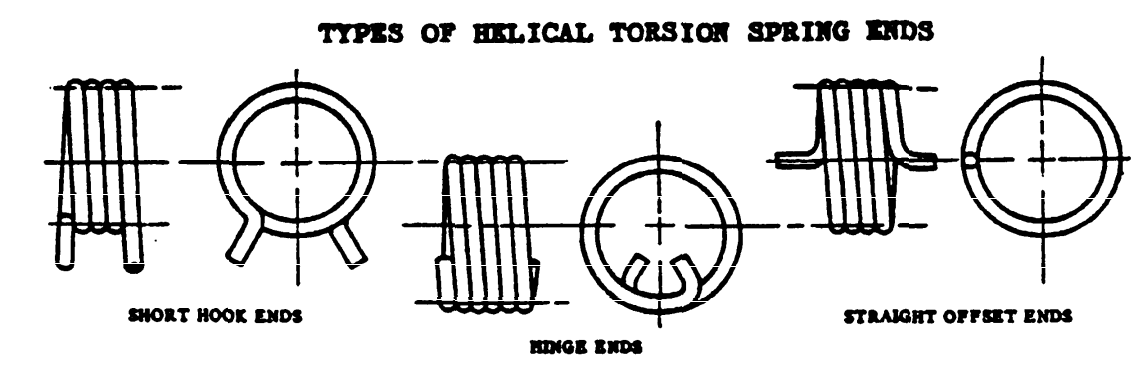
\includegraphics[width=0.8\textwidth]{milstd29a_fig8.png}
    \caption{}
    \label{fig:2d}
\end{figure}

\begin{figure}[htbp] % h:here, t:top, b:bottom, p:page
    \centering
    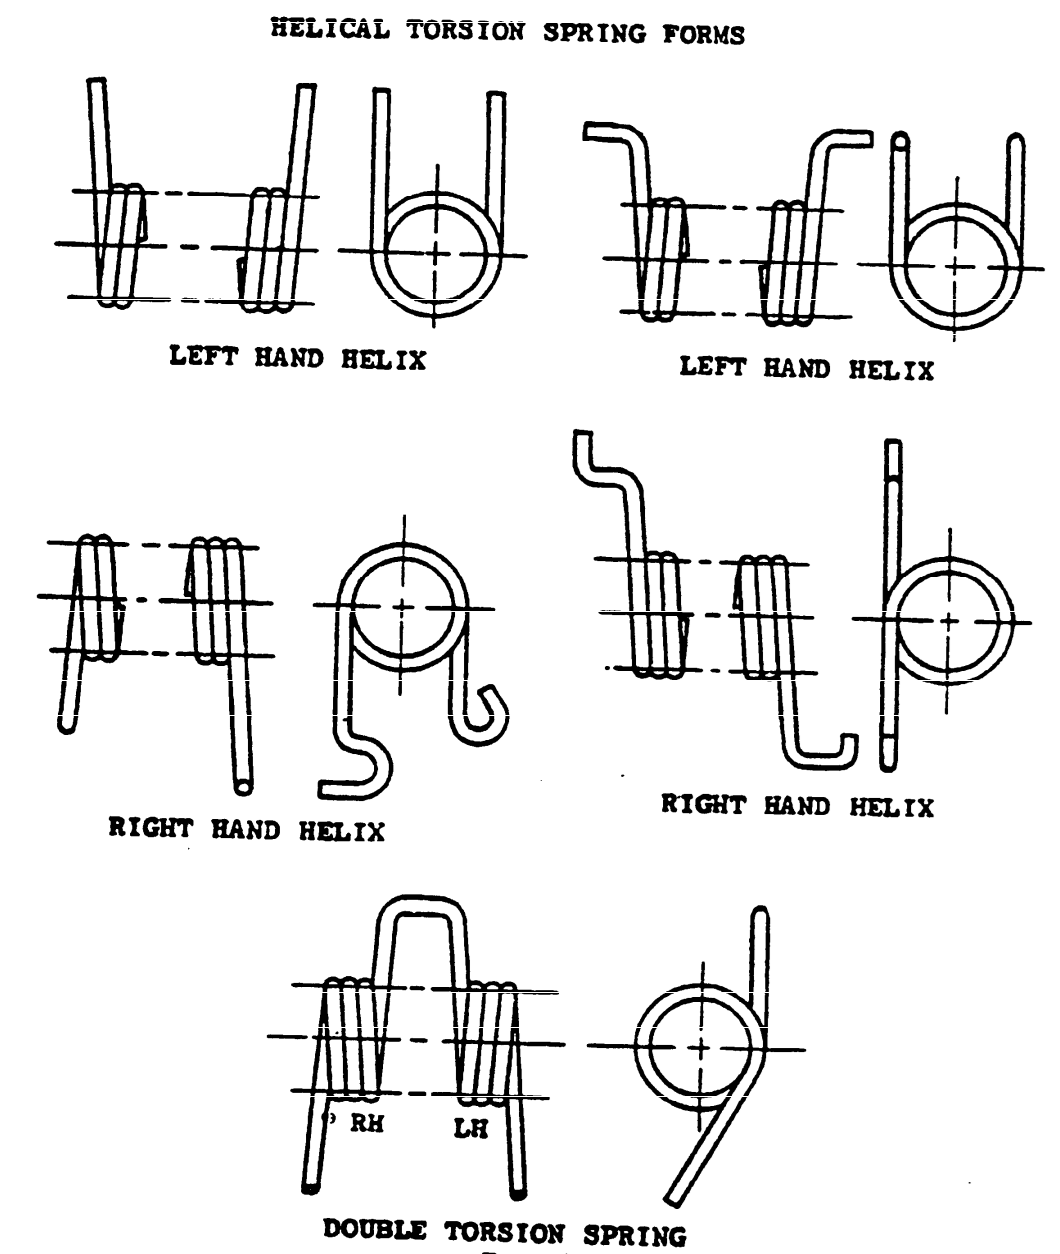
\includegraphics[width=0.8\textwidth]{milstd29a_fig9.png}
    \caption{}
    \label{fig:2d}
\end{figure}

% pg 22:
\clearpage
\subsection{Spiral Torsion Springs} % Section 5.8
\subsubsection{Definition} % Section 5.8.1
A spiral torsion spring is usually made by winding flat spring material on itself in the form of a spiral; and designed to wind up to exert pressure in a rotating direction around the spring axis.
This pressure may be delivered as torque or it may be converted into a push or a pull force.

\subsubsection{Drawing Requirements} % Section 5.8.2
(yet to be transcribed)

\paragraph{Outside and Inside Diameter of Coil} % Section 5.8.2.1
(yet to be transcribed)

\paragraph{Developed Length of Material and Active Length of Material} % Section 5.8.2.2
(yet to be transcribed)

\paragraph{Number of Coils in Free Position} % Section 5.8.2.3
(yet to be transcribed)

\paragraph{Type of Ends and Angular Relation of Ends} % Section 5.8.2.4
(yet to be transcribed)

\begin{figure}[htbp] % h:here, t:top, b:bottom, p:page
    \centering
    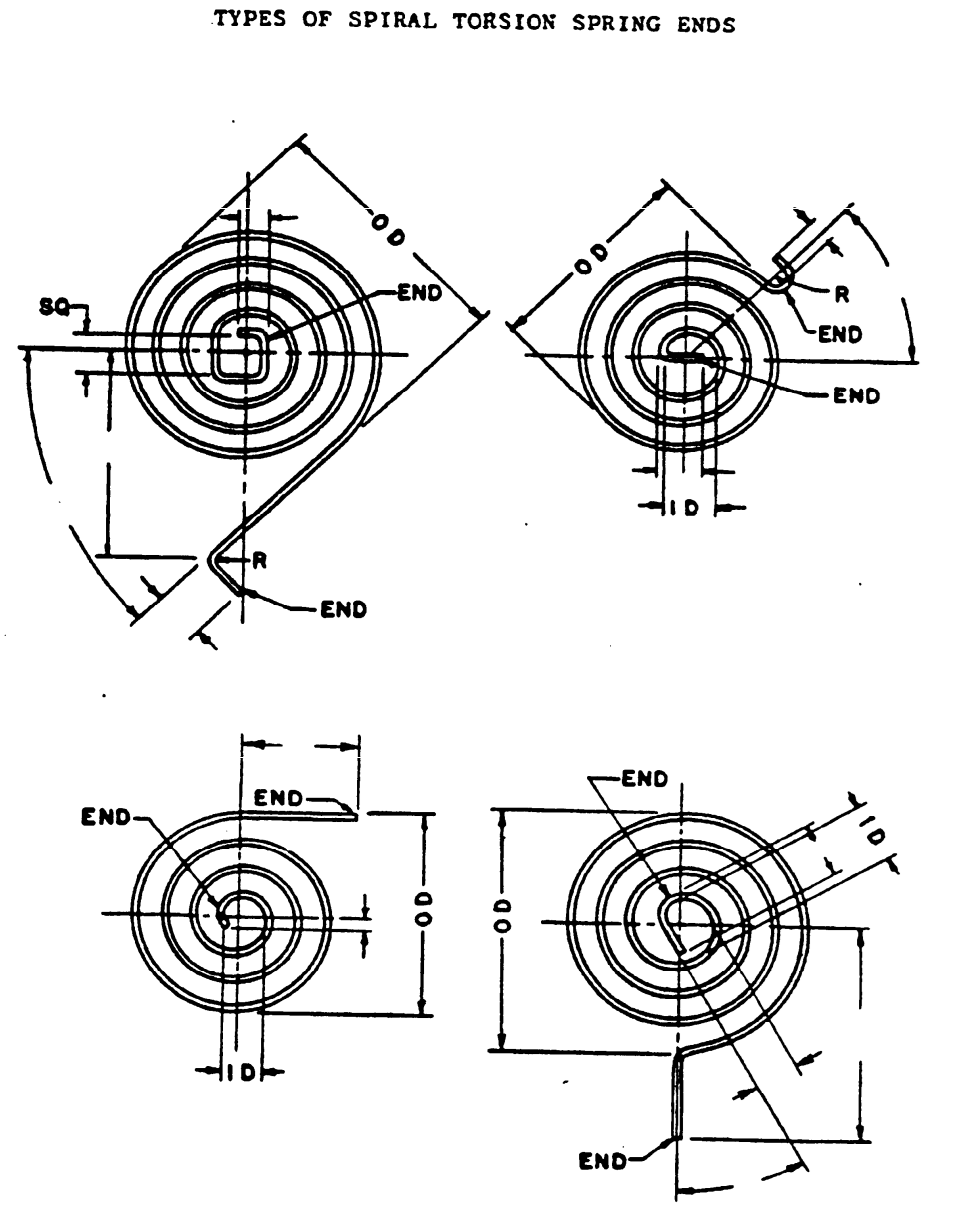
\includegraphics[width=0.8\textwidth]{milstd29a_fig11.png}
    \caption{}
    \label{fig:2d}
\end{figure}

\begin{figure}[htbp] % h:here, t:top, b:bottom, p:page
    \centering
    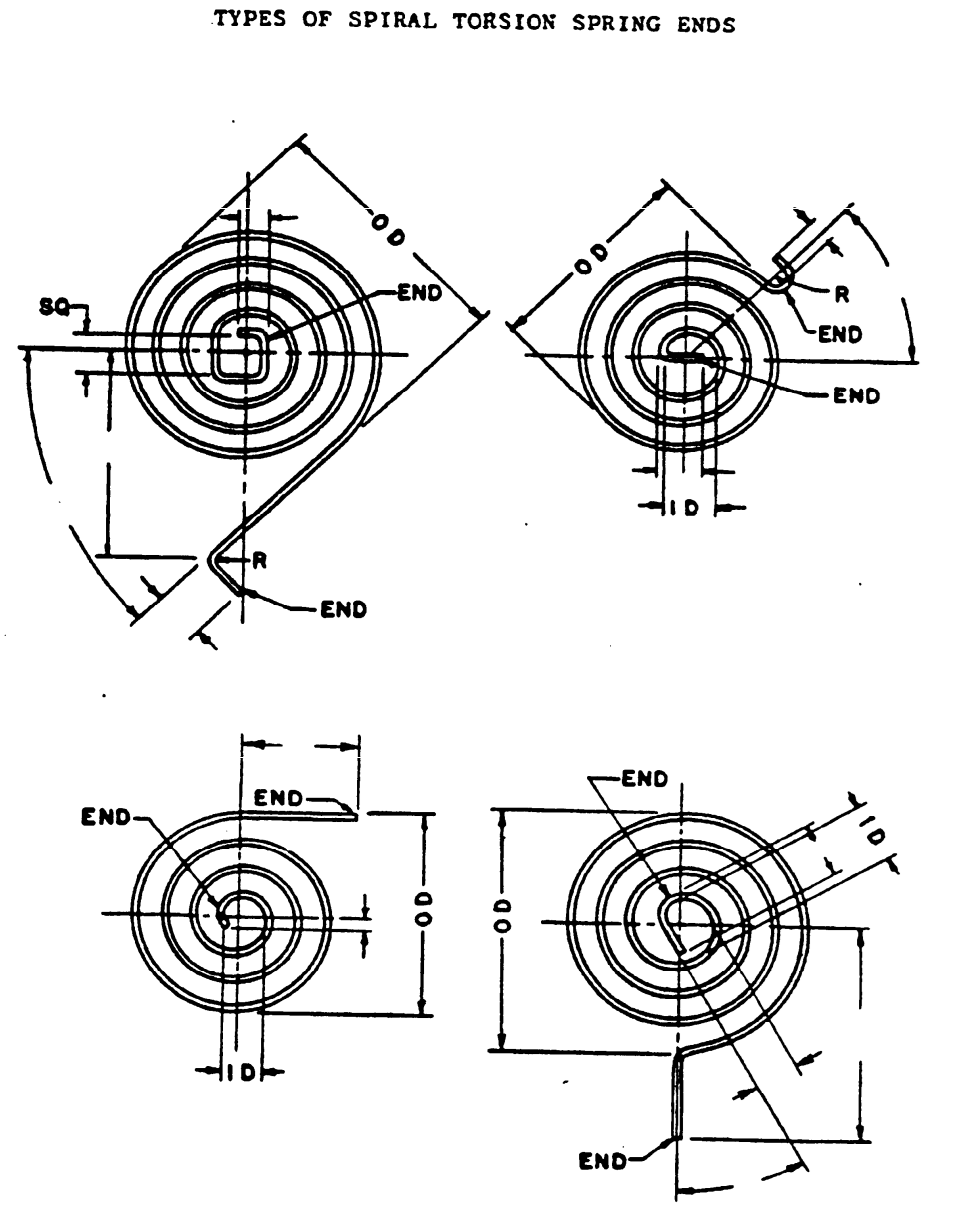
\includegraphics[width=0.8\textwidth]{milstd29a_fig11.png}
    \caption{}
    \label{fig:2d}
\end{figure}

% pg 24:
\clearpage
\subsection{Torsion Bar Springs} % Section 5.9
\subsubsection{Definition} % Section 5.9.1
Torsion bar springs are straight bars or rods of definite cross section used to offer a resistance to a twisting moment about the longitudinal axis. 
The cross section may be round, square, rectangular or hexagonal as dictated by design and availability. 
Circular cross-sections are generally used. 
Both ends are generally upset to diameters larger than the body diameters with a tapered transition section between body
and ends to keep stress concentrations to a minimum. 
Splines, serrations, or other types of couplings are cut on the upset ends to form the means of anchorage.

\subsubsection{Drawing Requirements for Torsion Bar Springs} % section 5.9.2
Explanation of the spring data listed in Figure 12 is given below. 
Figure 24 is a typical detail drawing of a torsion bar spring, and Figure 25 lists processing data.

\paragraph{Diameters of Body and Ends} % section 5.9.2.1
Specify in the delineation both the end diameter and the body diameter as tolerance dimensions.

\paragraph{Length Overall and of Ends} % section 5.9.2.2
Specify in the front view the overall length, and the length of ends, with tolerances.

\paragraph{Angle of Taper} % section 5.9.2.3
Specify the angle of taper with a tolerance in the front view.

\paragraph{Torque Loads} % section 5.9.2.4
The torque loads with tolerances should be specified in pound inches or pound feet, as appropriate, at definite
amounts of deflection in degrees of rotation from the free position. 
Torque loads should preferably be specified at the initial and the final operating positions in the assembly.

\paragraph{Spring Rate} % section 5.9.2.5
Specify the spring rate in lb in./degree or lb ft/degree, as a REFERENCE.

\paragraph{Type of Ends} % section 5.9.2.6
The type of end (involute spline, serrations, etc. ) shall be completely delineated and dimensioned on detail drawings.

\paragraph{Direction of Windup Marking} % section 5.9.2.7
For coldset torsion bar springs, the direction of windup (load application in service) shall be indicated with an arrow on the end of the spring. 
For torsion bar springs which are not coldset, direction of windup marking is not required.

\paragraph{Angular Relation between Ends} % section 5.9.2.8
For torsion bar springs which are coldset a scribe line (approximately 1/16 x 60°V) shall be cut on each end of the spring. The end view shall show the angular relation between the ends before and after coldsetting. 
For torsion bar springs which are not coldset, angular relation between ends is not required unless an angular relation must be maintained between involute spline or serration teeth.

\begin{figure}[htbp] % h:here, t:top, b:bottom, p:page
    \centering
    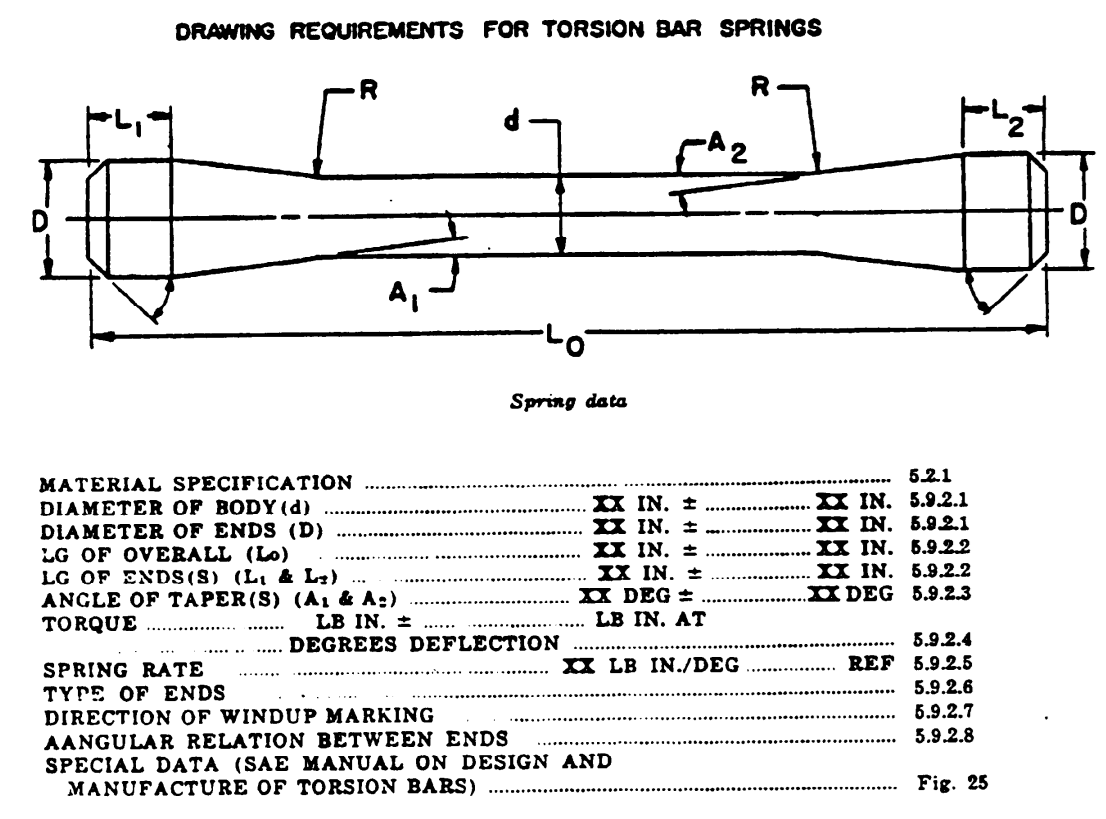
\includegraphics[width=0.8\textwidth]{milstd29a_fig12.png}
    \caption{}
    \label{fig:2d}
\end{figure}

% pg 25:
\clearpage
\subsection{Volute Springs} % Section 5.10
\subsubsection{Definition}% Section 5.10.1
Volute Springs are conical shaped compression springs made of rectangular cross-sectional material so constructed
that the coils are capable of telescoping into each other.

\subsubsection{Drawing Requirements} % Section 5.10.2
Explanation of the spring data listed in Figure 13 is given below. 
Figure 26 is a typical detail drawing of a volute spring.

\paragraph{Outside and Inside Diameter} % Section 5.10.2.1
Specify in the delineation both the outside and the inside diameters as tolerance dimensions.

\paragraph{Free Length} % Section 5.10.2.2
Specify the free length as a REFERENCE dimension in the delineation.

\paragraph{Total Coils} % Section 5.10.2.3
Specify the number of total coils, as a REFERENCE, or with a tolerance if essential to the design.

\paragraph{Radial Pitch} % Section 5.10.2.4
Specify the radial pitch in inches with a tolerance.

\paragraph{Axial Pitch and Helix Angle} % Section 5.10.2.5
The axial pitch and the helix angle of a volute spring determine its loads, length and bottoming characteristics. 
Volute springs with a constant axial pitch will have the largest active coil bottoming first. 
A spring with a constantly reducing axial pitch will have a smaller pitch for the smaller coils and such springs can be designed so that all active coils theoretically bottom at about the same time.
Specify either the helix angle or prefereably the axial pitch with a tolerance as constant.
If the helix angle is constant the pitch will vary; if the pitch is constant, the helix angle will vary.
It is impossible because of the nature of the spring to have both the helix angle and the pitch as constant.
However, it is possible for both pitch and helix angle to vary throughouta volute spring.

\paragraph{Loads} % Section 5.10.2.6
Specify the loads with tolerances to be developed at definite compressed lengths, prefereably at the initial and the final operating positions in the assembly.

\paragraph{Solid Length}
Specify the solid length as a maximum dimension allowing for the tolerance on the width of the blade, protective coating, etc. 
The spring should not ordinarily be permitted to go solid in operation, except when used as a bumper or dictated by
other design requirements.

\begin{figure}[htbp] % h:here, t:top, b:bottom, p:page
    \centering
    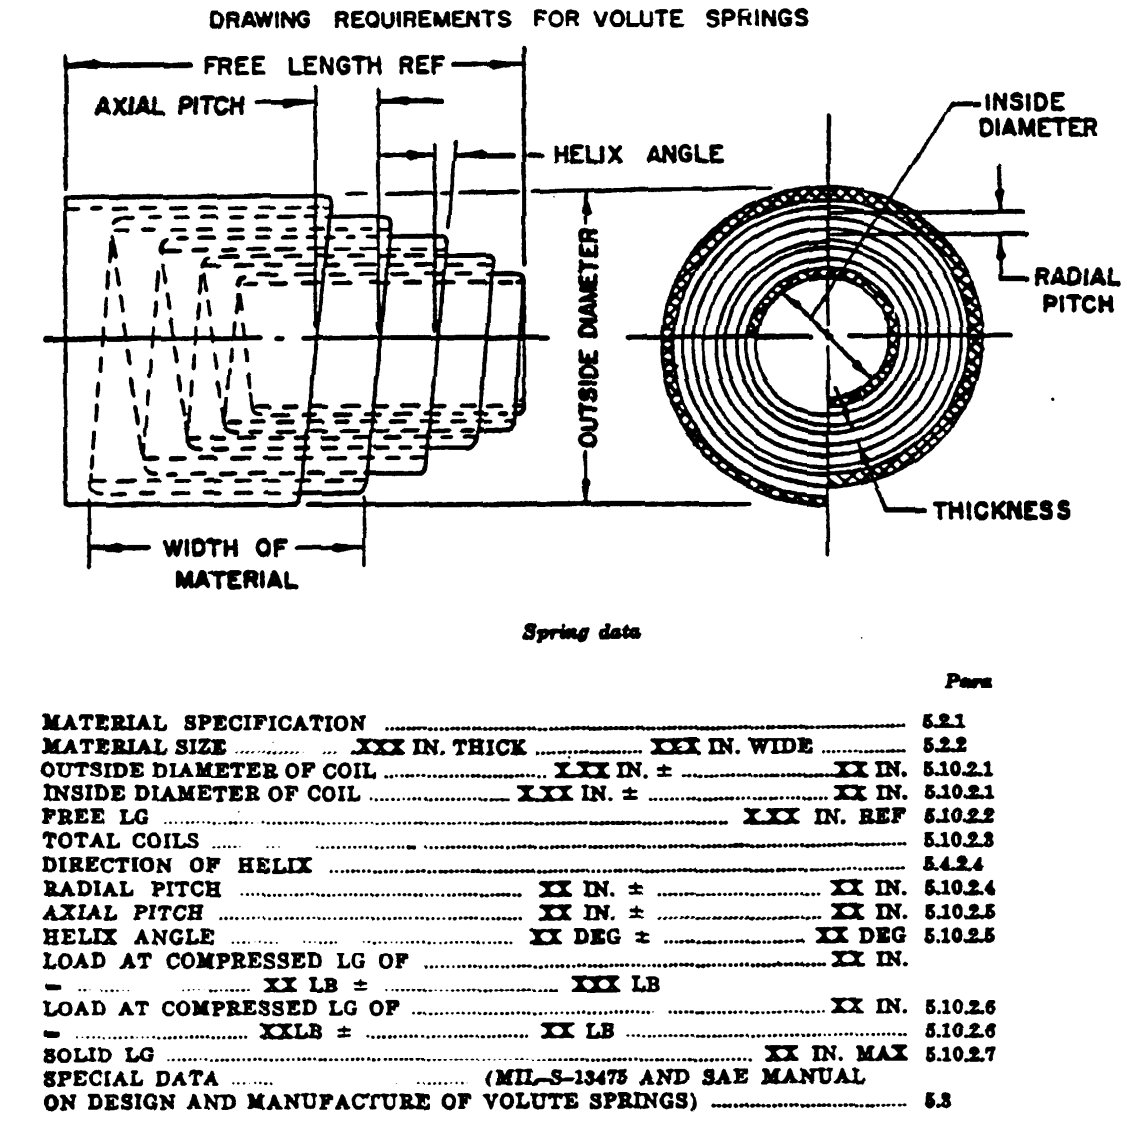
\includegraphics[width=0.8\textwidth]{milstd29a_fig13.png}
    \caption{}
    \label{fig:2d}
\end{figure}

% pg 27:
\clearpage
\subsection{Coned Disc Belleville Springs} % Section 5.11
\subsubsection{Definition} % Section 5.11.1
A coned disc (Belleville) spring is a spring washer in the form of a frustum of a cone, having constant material thickness, and used as a compression spring.

\subsubsection{Drawing Requirements for Coned Disc (Belleville) Springs} % Section 5.11.2
Explanation of the spring data listed in Figure 14 is given below. 
Figure 27 is a typical detail drawing of a coned disc (Belleville) spring.

\paragraph{Inside and Outside Diameters} % Section 5.11.2.1
(yet to be transcribed)

\paragraph{Free Height and Method of Stacking} % Section 5.11.2.2
(yet to be transcribed)

\paragraph{Loads} % Section 5.11.2.3
When discs are to be installed singularly, only one load with a tolerance applied shall be specified. 
When discs are to be installed in sets, specify the loads with a tolerance at definite compreeaed kn~ preferably at the Mid ~d m o-g
poaitiona Uf the U=hmiQn
When discs are used in sets, a load for individual discs shall not be specified. 
When discs are used in sets, the following note shall be included on detail drawings:

STACKS SHALL BE SECURED TOGETHER IN THE SEQUENCE OF TESTING AND SUCH SEQUENCE SHALL BE RETAINED UPON INSTALLATION

\paragraph{Bearing Surfaces} % Section 5.11.2.4
Bearing surfaces may be provided when necessary to meet the design requirements. 
They aid in meeting tests for loads, tolerances and burr removal.
They should not exceed .080 inches wide.

\paragraph{Bearing Surfaces Parallel} % Section 5.11.2.5
Such surfaces must be parallel in an amount equal to or less than 15\% of the Free Height, when measured at a distance of twice the Outside Diameter, located from the center line.

\paragraph{Concentricity between Outside and Inside Diameters} % Section 5.11.2.6
Specify the concentricity between the outside and inside diameters when important. 
When specified, the outside diameter of the springs shall be concentric with the inside diameter within .008 inches
(.006 TIR) for springs 2 inches and less in outside diameter, and .005 inches (.010 TIR) for springs over 2 inches in outside diameter.

\begin{figure}[htbp] % h:here, t:top, b:bottom, p:page
    \centering
    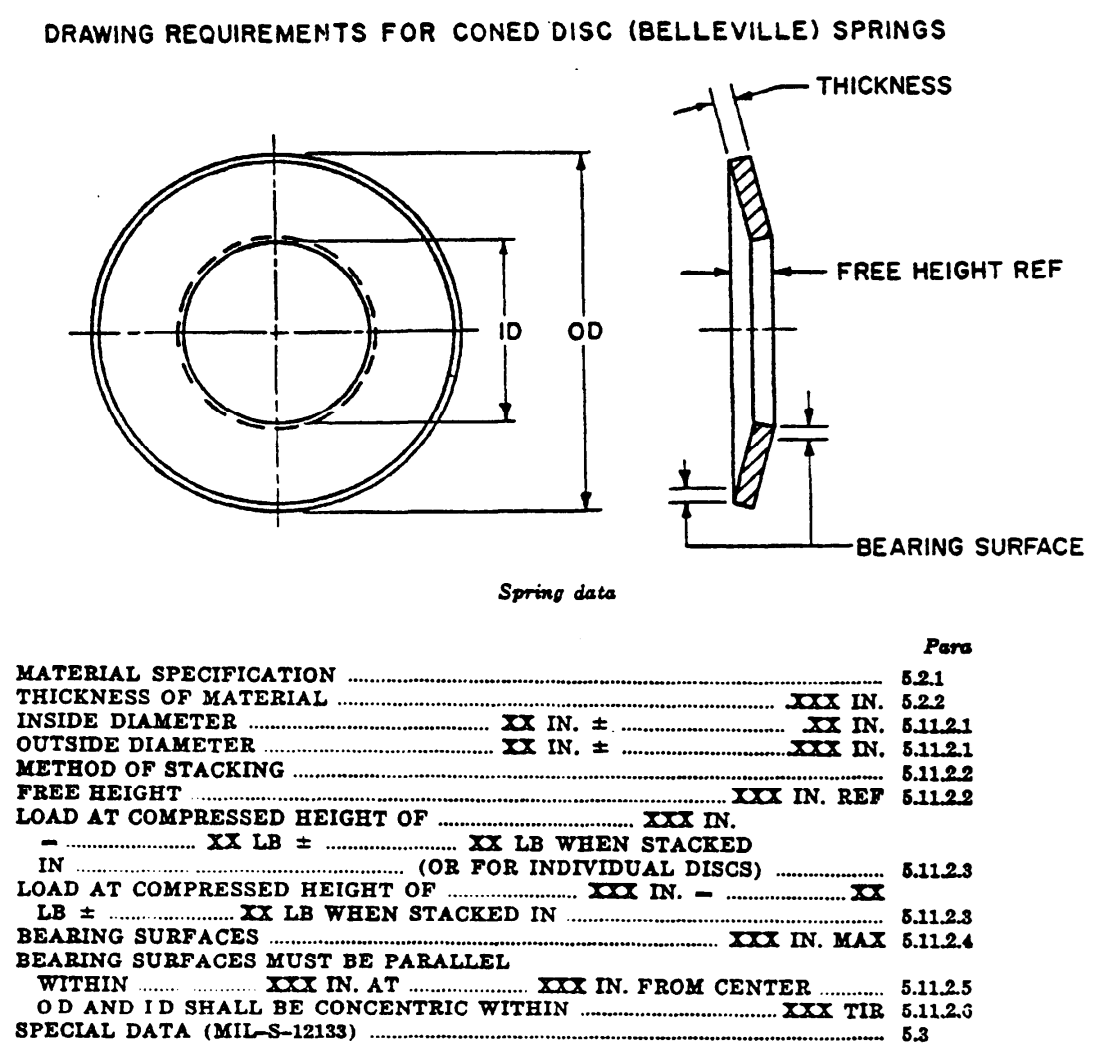
\includegraphics[width=0.8\textwidth]{milstd29a_fig14.png}
    \caption{}
    \label{fig:2d}
\end{figure}

\begin{figure}[htbp] % h:here, t:top, b:bottom, p:page
    \centering
    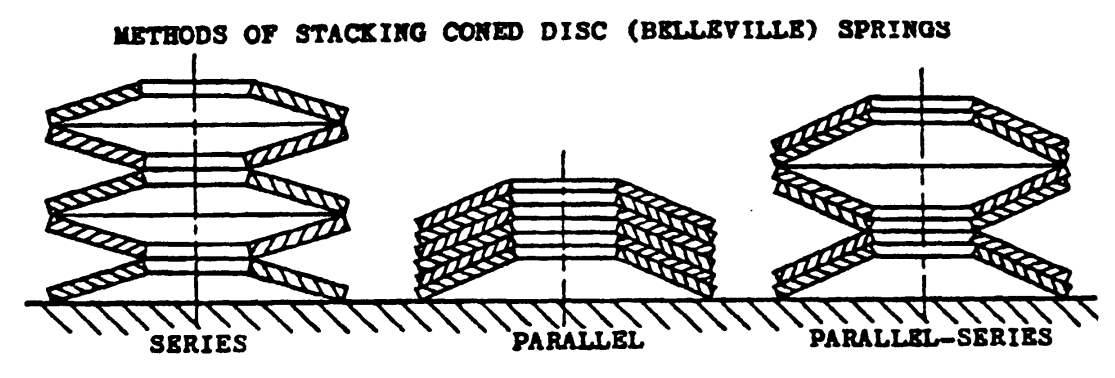
\includegraphics[width=0.8\textwidth]{milstd29a_fig15.png}
    \caption{}
    \label{fig:2d}
\end{figure}

\clearpage
\subsection{Flat Springs} % Section 5.12
(yet to be transcribed)

\subsubsection{Definition}
(yet to be transcribed)

\subsubsection{Drawing Requirements}
(yet to be transcribed)

\paragraph{Developed Lengths}
(yet to be transcribed)

\paragraph{Clamp Length}
(yet to be transcribed)

\paragraph{Loads}
(yet to be transcribed)

\begin{figure}[htbp] % h:here, t:top, b:bottom, p:page
    \centering
    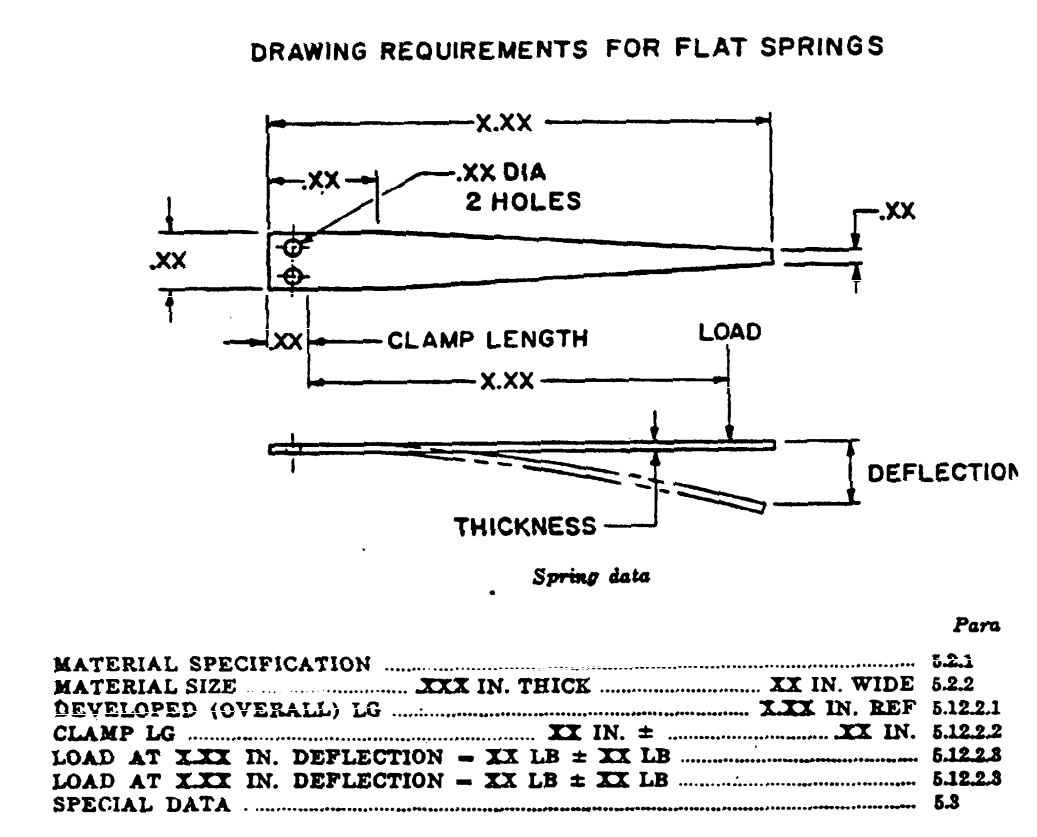
\includegraphics[width=0.8\textwidth]{milstd29a_fig16.png}
    \caption{}
    \label{fig:2d}
\end{figure}

\clearpage
\subsection{Constant Force Springs} % Section 5.13
(yet to be transcribed)

\subsubsection{Definition} % Section 5.13.1
(yet to be transcribed)

\subsubsection{Drawing Requirements} % Section 5.13.2
(yet to be transcribed)

\paragraph{Loads}
(yet to be transcribed)

\paragraph{Initial Position and Final Position}
(yet to be transcribed)

\paragraph{Type of Ends}
(yet to be transcribed)

\paragraph{Fits Over Roller}
(yet to be transcribed)

\paragraph{Thickness}
(yet to be transcribed)

\begin{figure}[htbp] % h:here, t:top, b:bottom, p:page
    \centering
    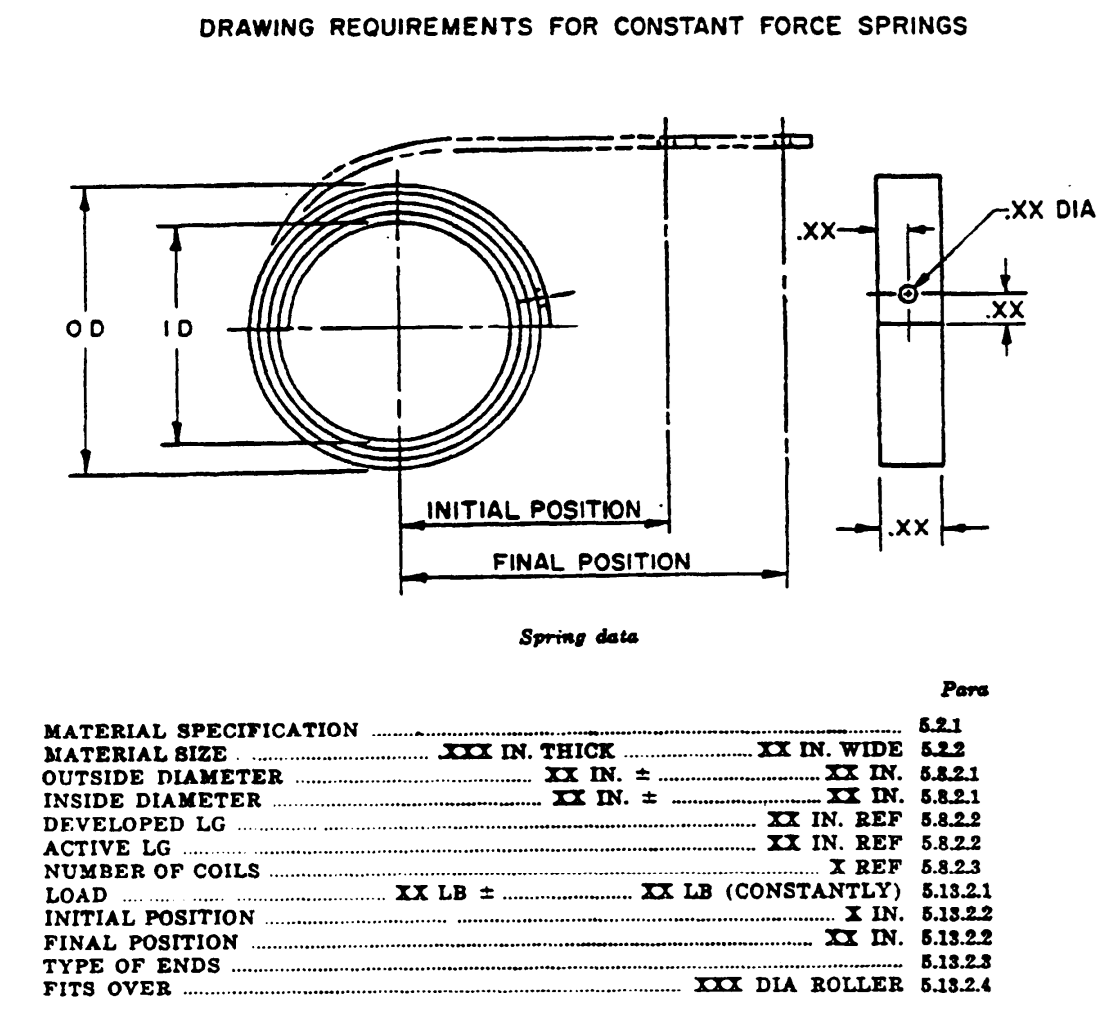
\includegraphics[width=0.8\textwidth]{milstd29a_fig17.png}
    \caption{}
    \label{fig:2d}
\end{figure}

\clearpage
\subsection{Garter Springs} % Section 5.14
\subsubsection{Definition} % Section 5.14.1
A garter spring is a special close coiled, long, extension spring with its ends fastened together and used in the form
of a ring. 
Such springs are used principally in mechanical seals on shafting; to hold round segments together; as belts and as
holding devices. 
It is customary to order the spring in straight lengths and fasten the ends at assembly.

\subsubsection{Drawing Requirements for Garter Springs} % Section 5.14.2
Explanation of the spring data listed in Figure 18 is given below. 
Figure 30 is a typical detail drawing of a garter spring.

\paragraph{Shaft Diameter} % Section 5.14.2.1
Specify the shaft diameter over which the spring works as a REFERENCE dimension.

\paragraph{Compressive Load per Inch of Circumference on Shaft} % Section 5.14.2.2
Specify this load as a REFERENCE only if essential to the design.

\begin{figure}[htbp] % h:here, t:top, b:bottom, p:page
    \centering
    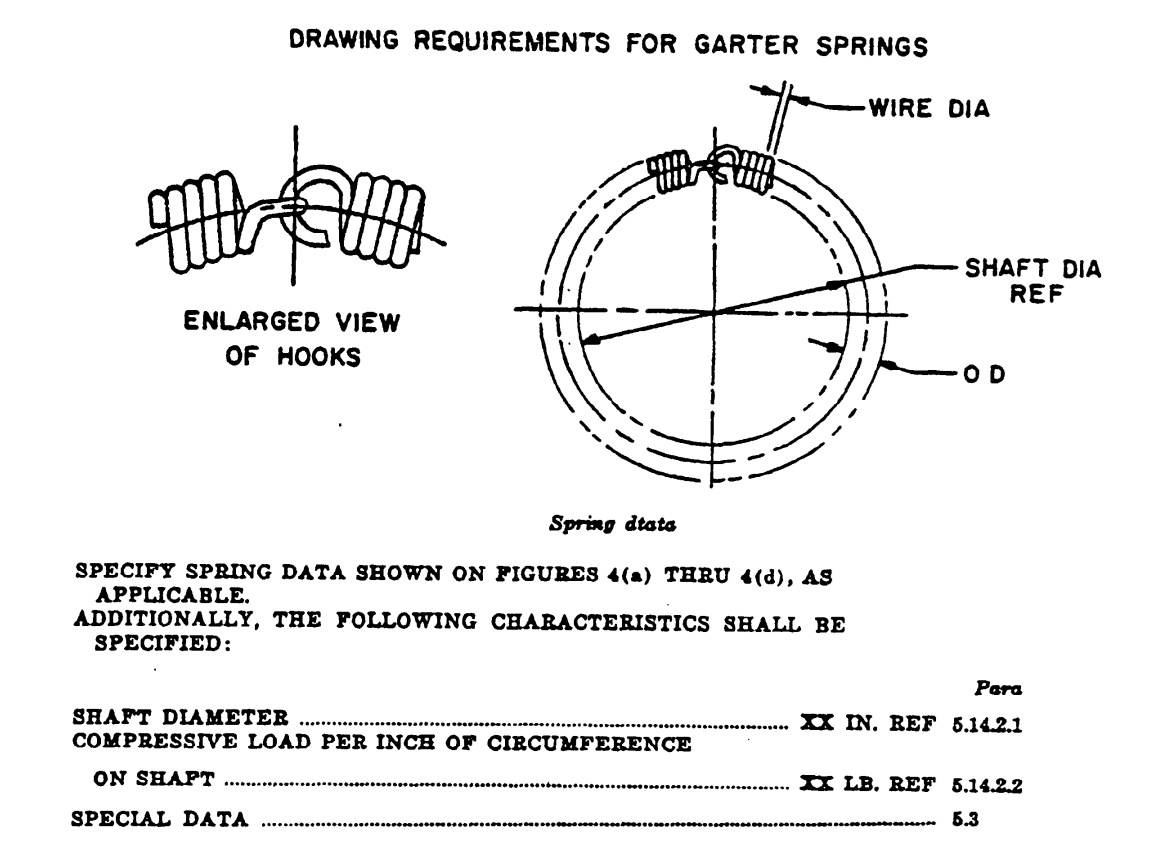
\includegraphics[width=0.8\textwidth]{milstd29a_fig18.png}
    \caption{}
    \label{fig:18}
\end{figure}

\clearpage

\begin{figure}[htbp] % h:here, t:top, b:bottom, p:page
    \centering
    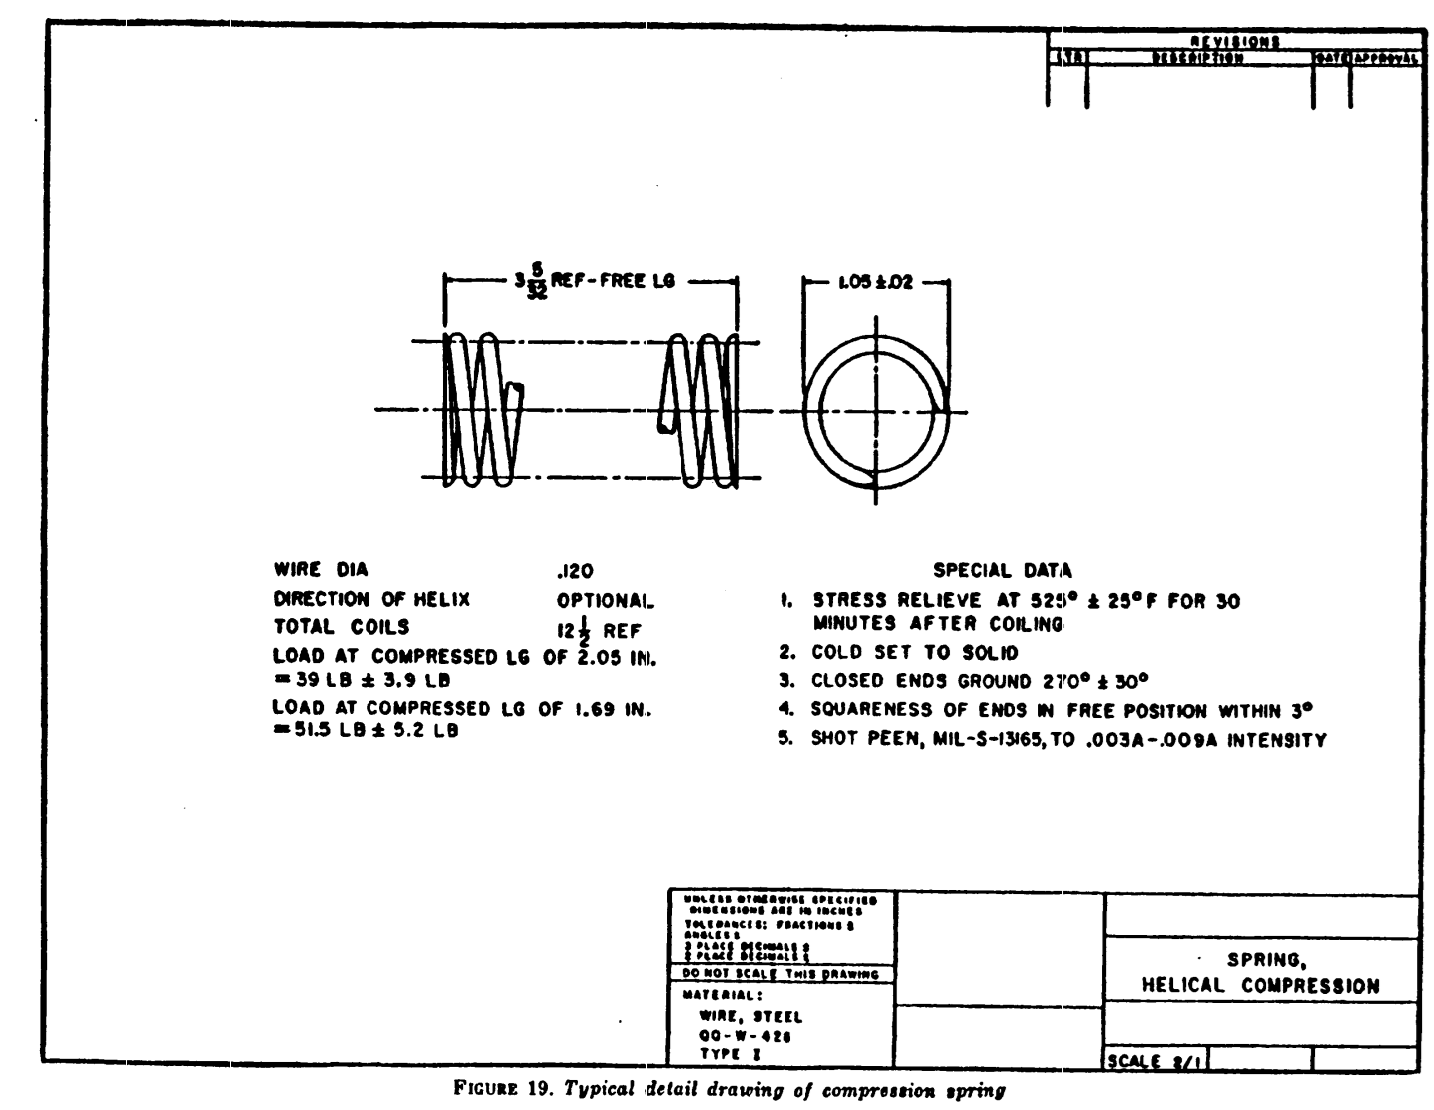
\includegraphics[width=0.8\textwidth]{milstd29a_fig19.png}
    \caption{}
    \label{fig:19}
\end{figure}

\begin{figure}[htbp] % h:here, t:top, b:bottom, p:page
    \centering
    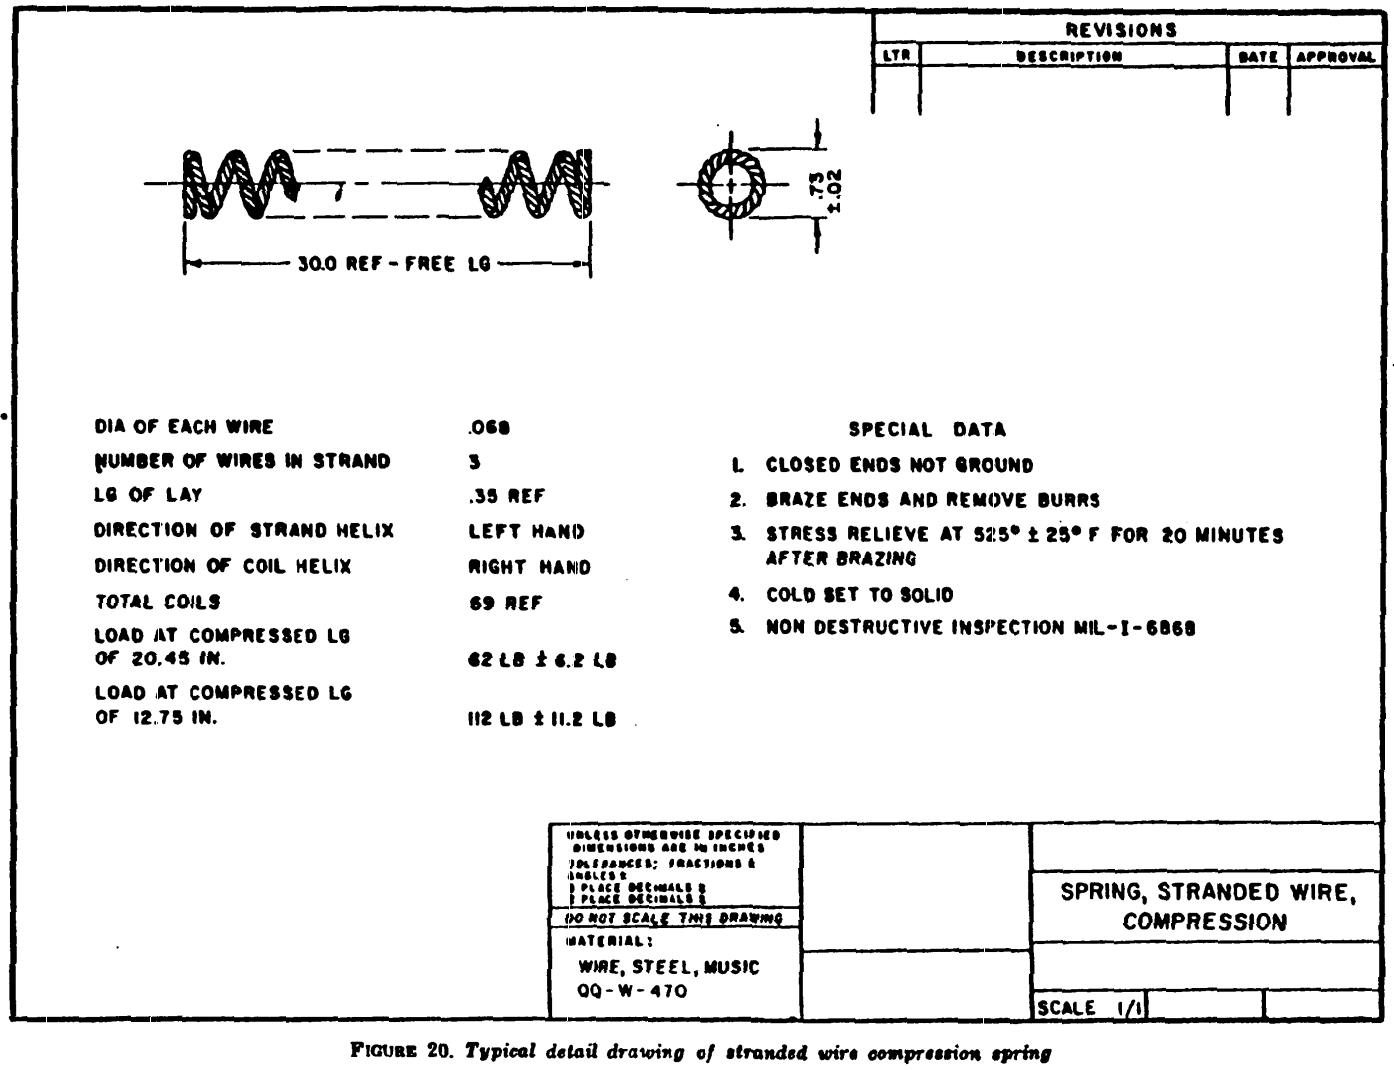
\includegraphics[width=0.8\textwidth]{milstd29a_fig20.png}
    \caption{}
    \label{fig:20}
\end{figure}

\begin{figure}[htbp] % h:here, t:top, b:bottom, p:page
    \centering
    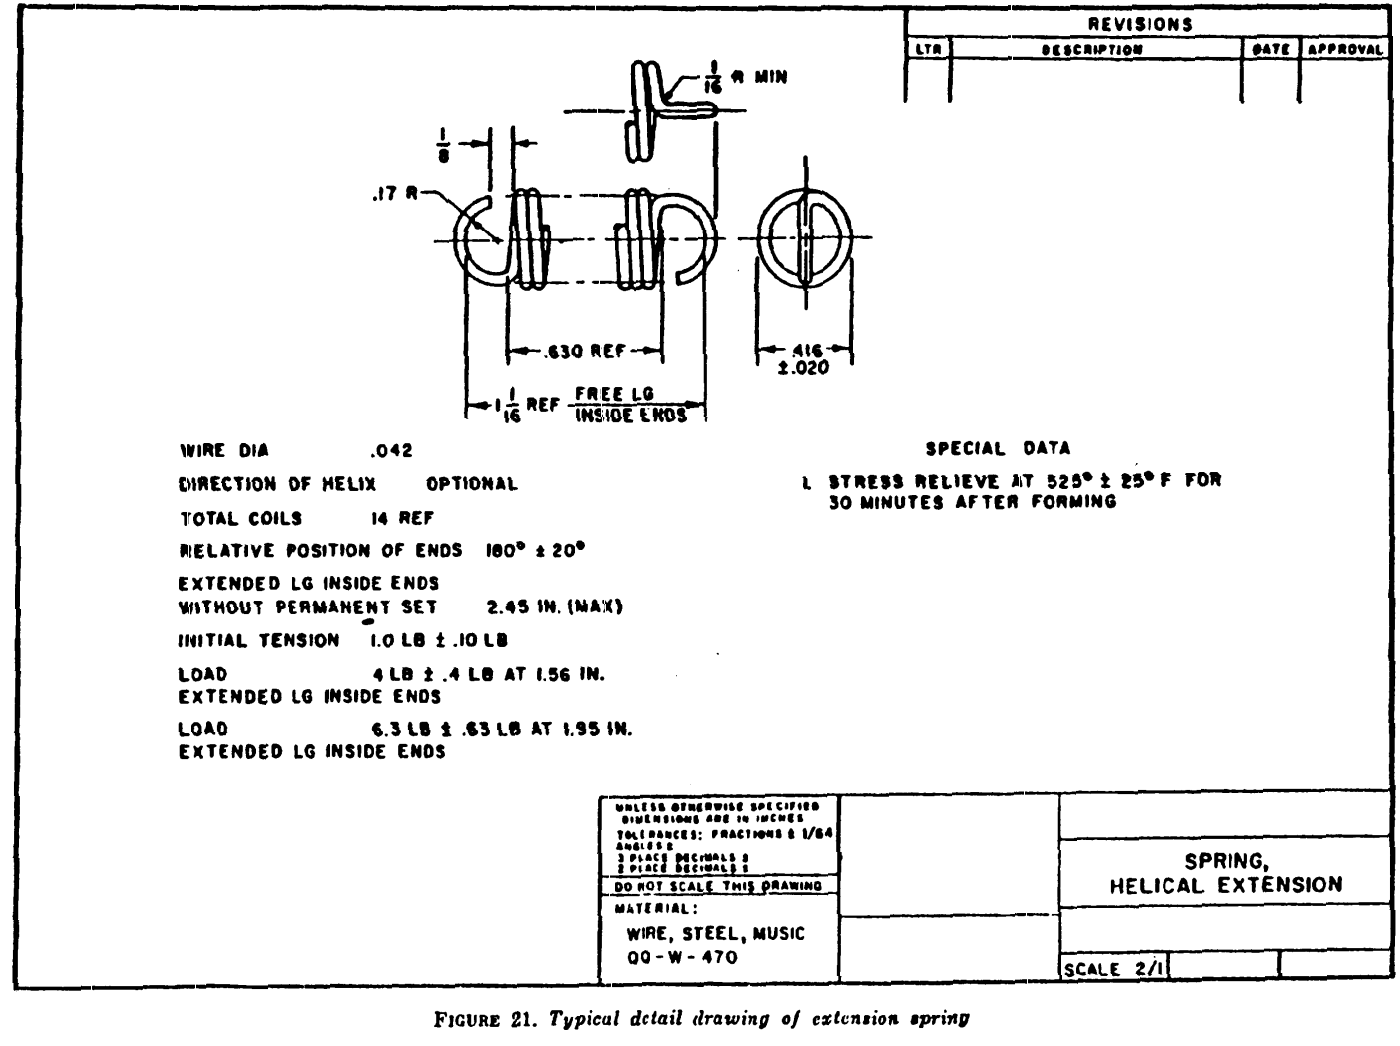
\includegraphics[width=0.8\textwidth]{milstd29a_fig21.png}
    \caption{}
    \label{fig:21}
\end{figure}

\begin{figure}[htbp] % h:here, t:top, b:bottom, p:page
    \centering
    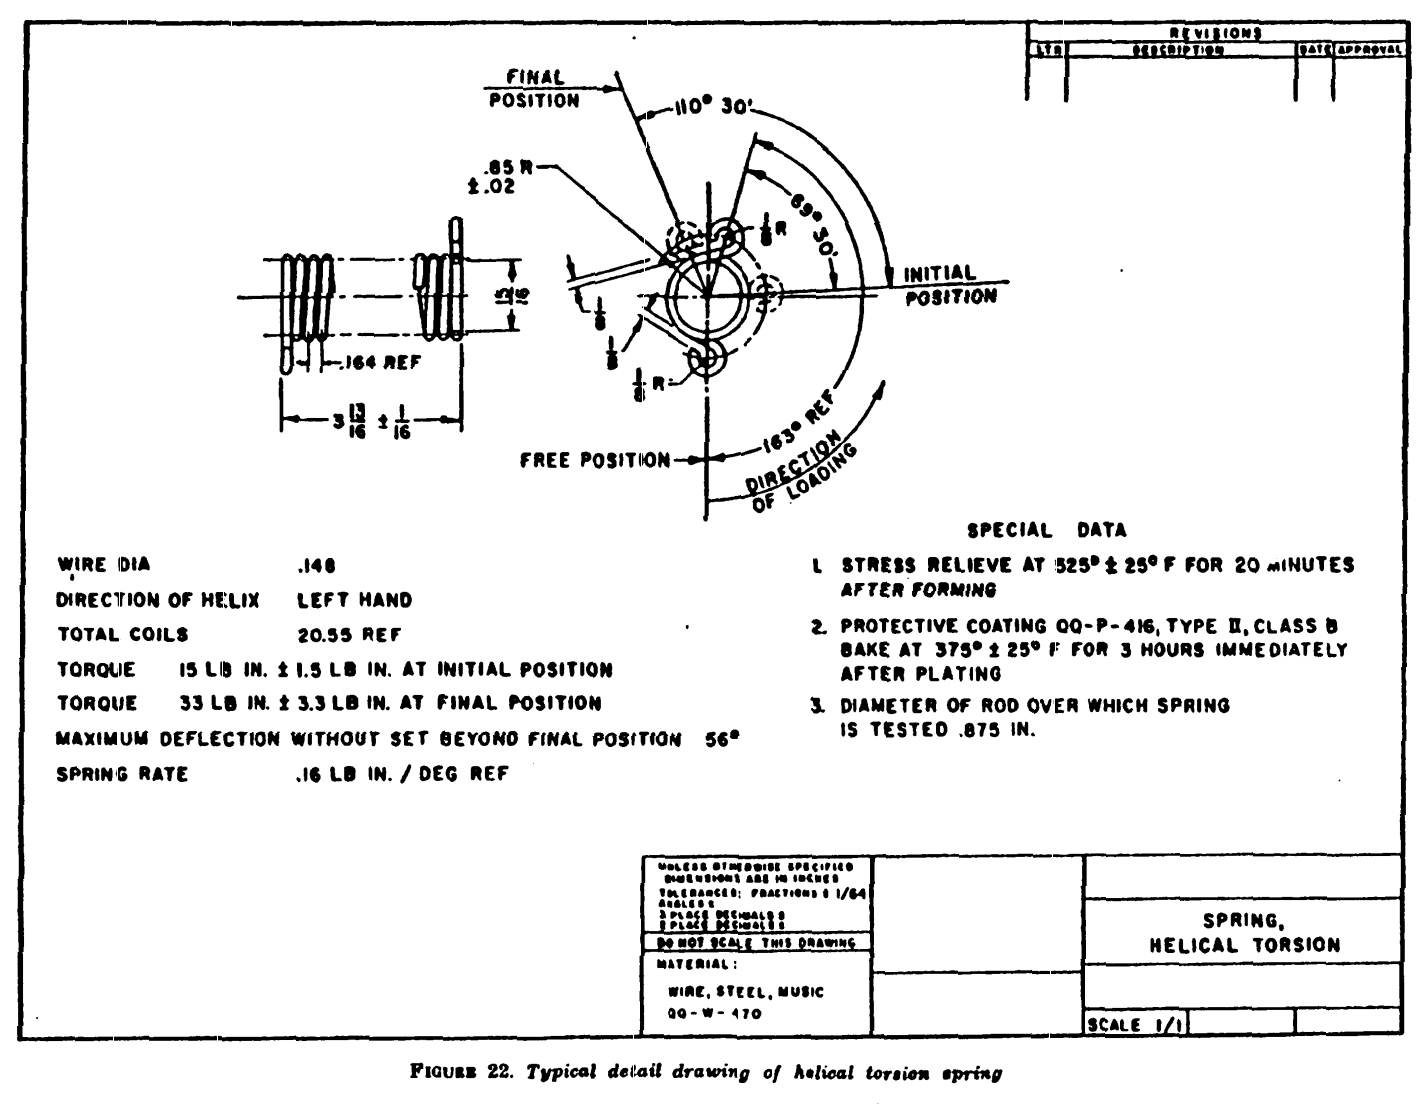
\includegraphics[width=0.8\textwidth]{milstd29a_fig22.png}
    \caption{}
    \label{fig:22}
\end{figure}

\begin{figure}[htbp] % h:here, t:top, b:bottom, p:page
    \centering
    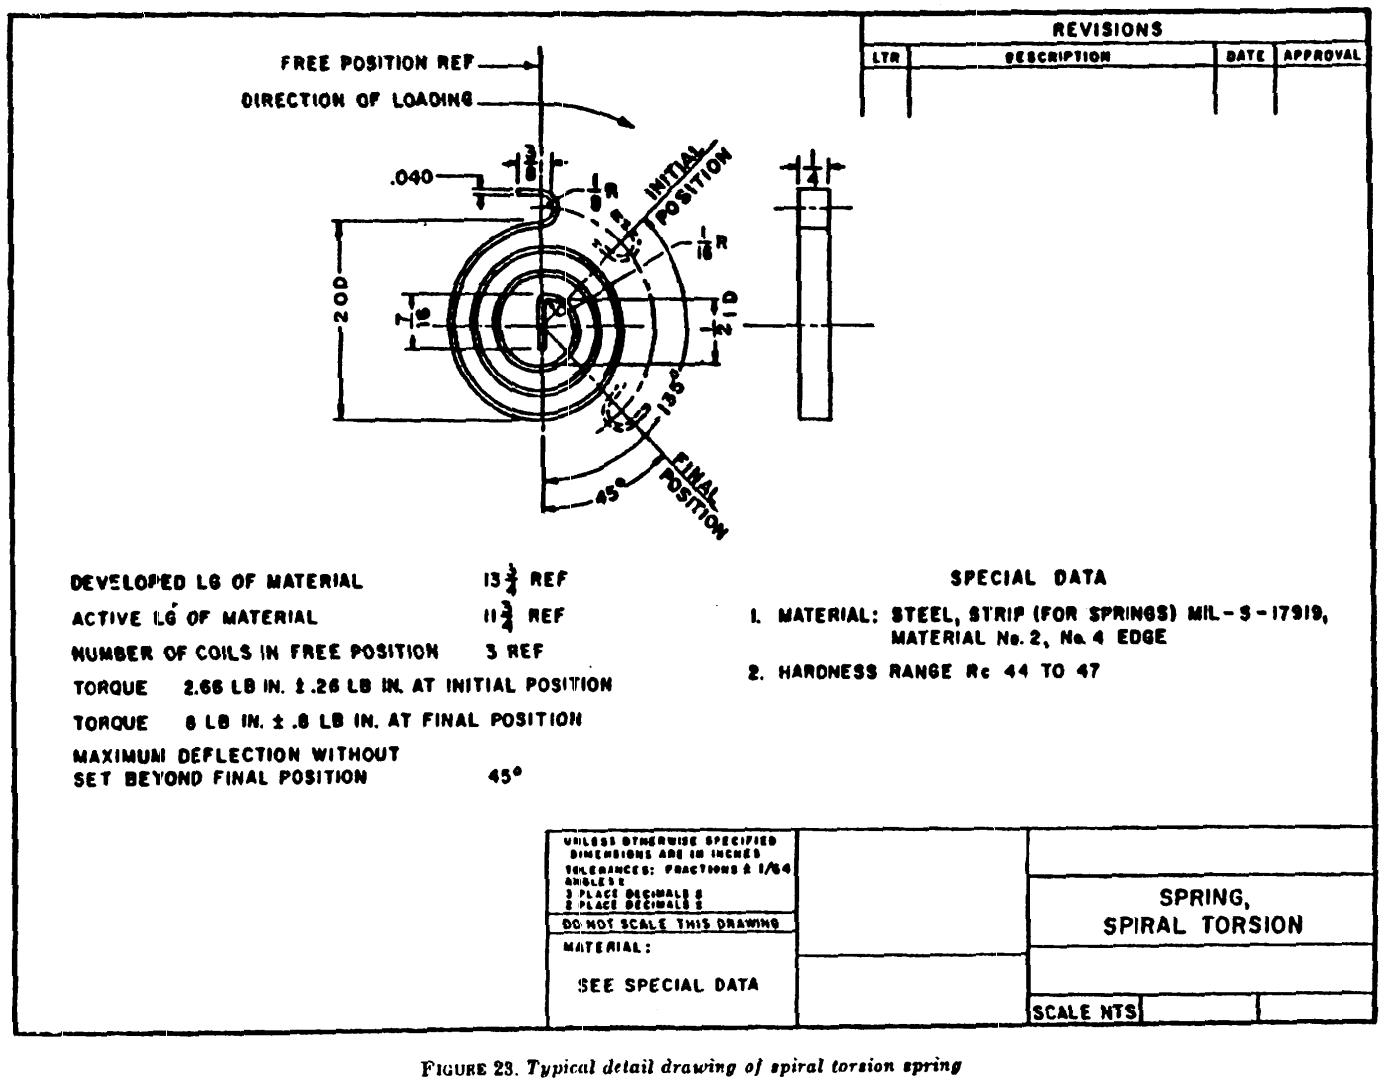
\includegraphics[width=0.8\textwidth]{milstd29a_fig23.png}
    \caption{}
    \label{fig:23}
\end{figure}

\begin{figure}[htbp] % h:here, t:top, b:bottom, p:page
    \centering
    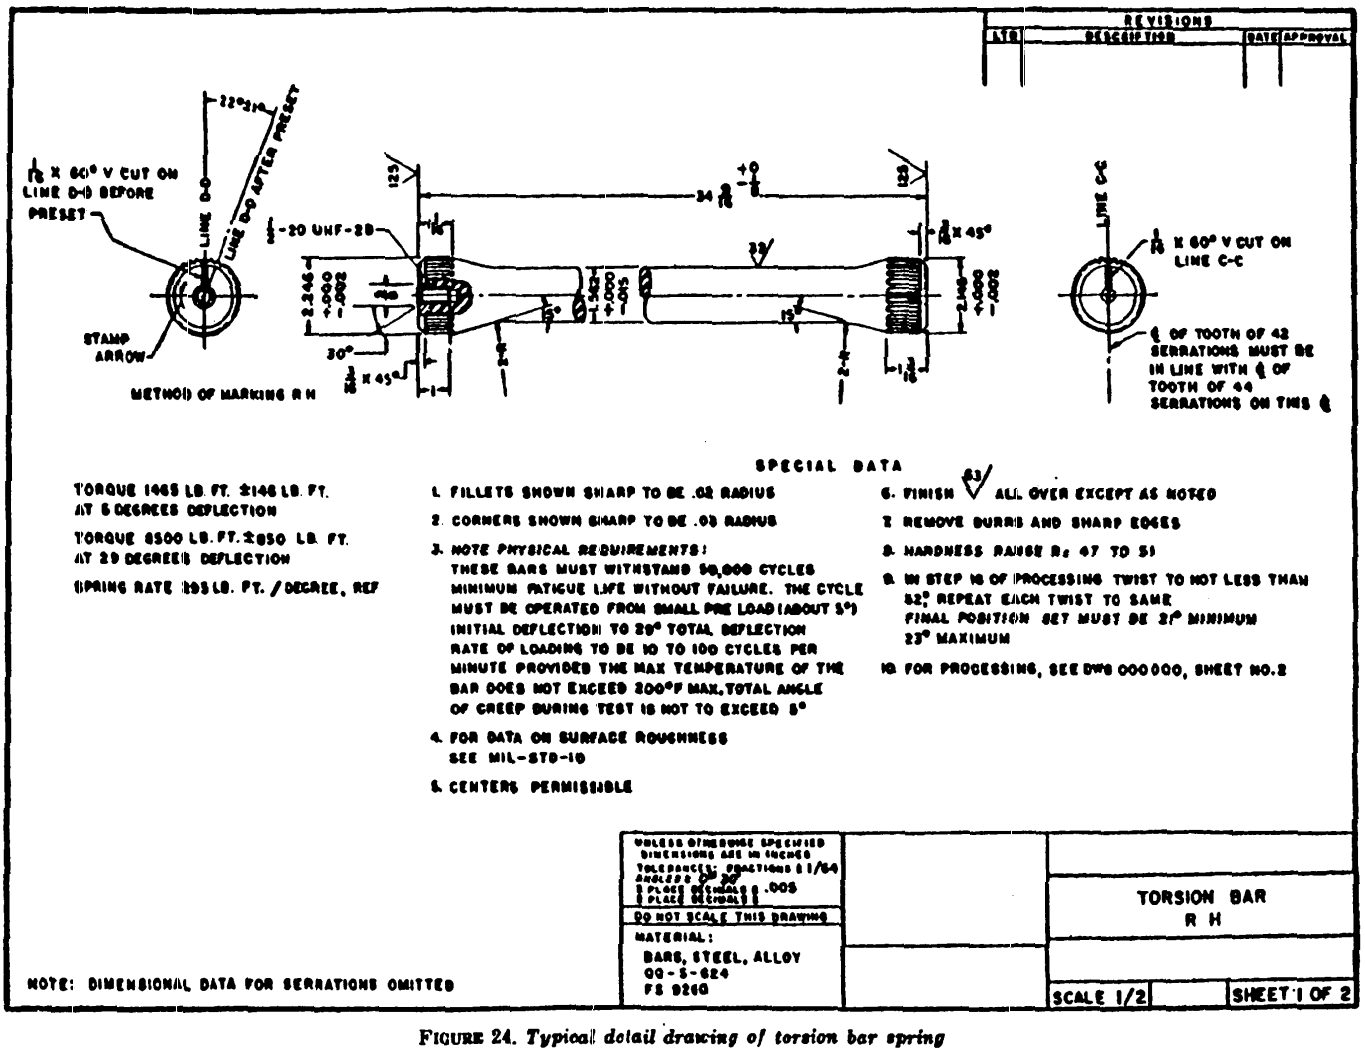
\includegraphics[width=0.8\textwidth]{milstd29a_fig24.png}
    \caption{}
    \label{fig:24}
\end{figure}

\begin{figure}[htbp] % h:here, t:top, b:bottom, p:page
    \centering
    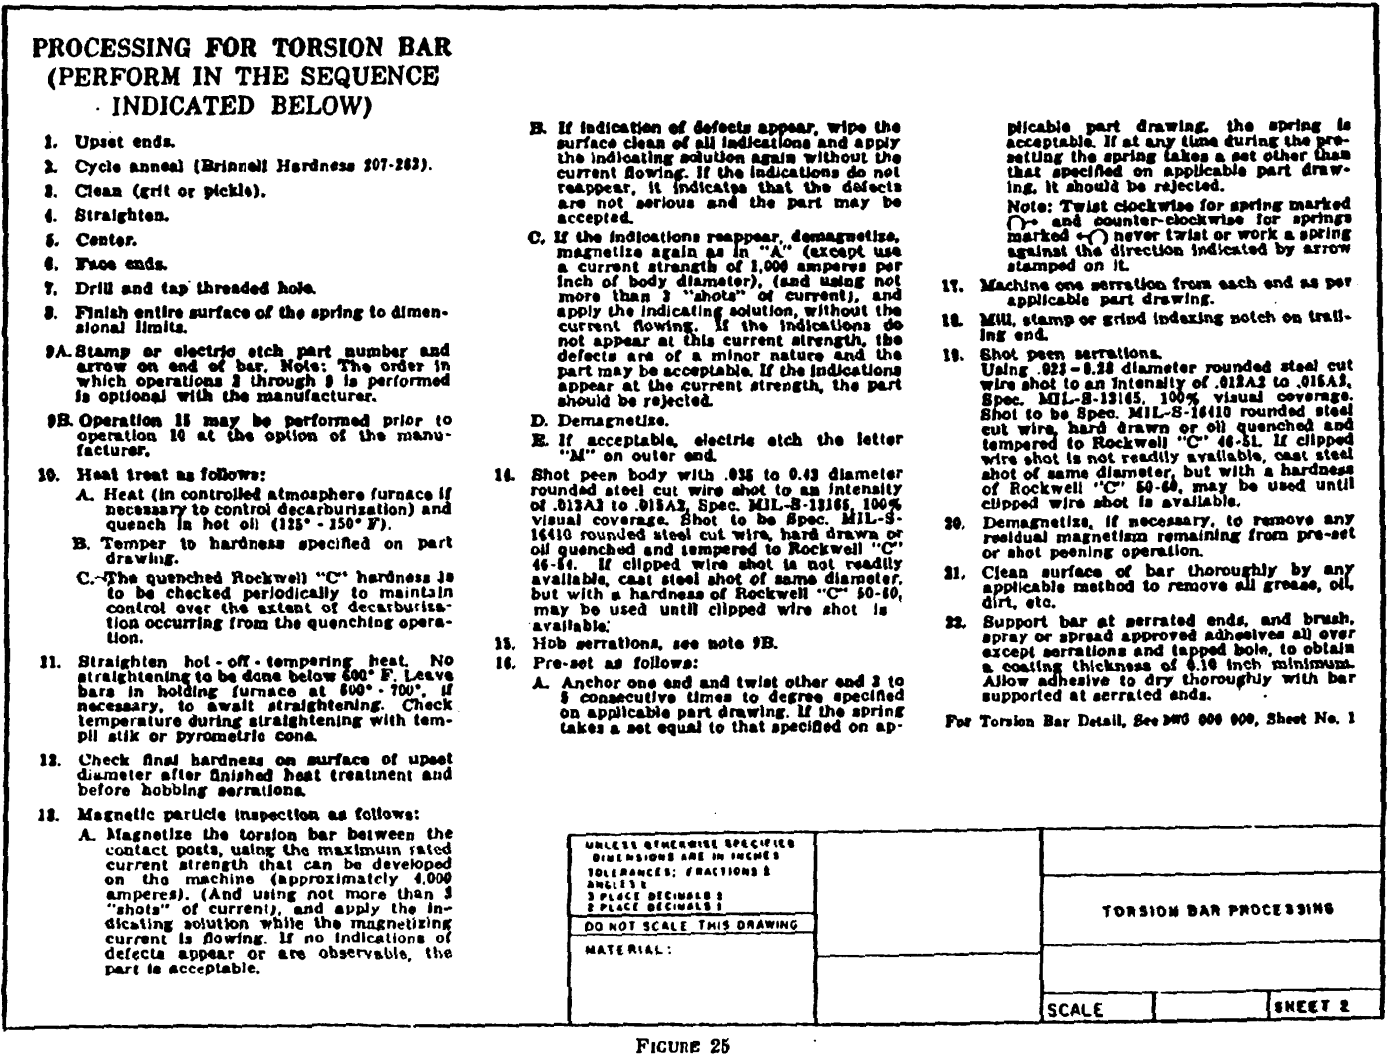
\includegraphics[width=0.8\textwidth]{milstd29a_fig25.png}
    \caption{}
    \label{fig:25}
\end{figure}

\begin{figure}[htbp] % h:here, t:top, b:bottom, p:page
    \centering
    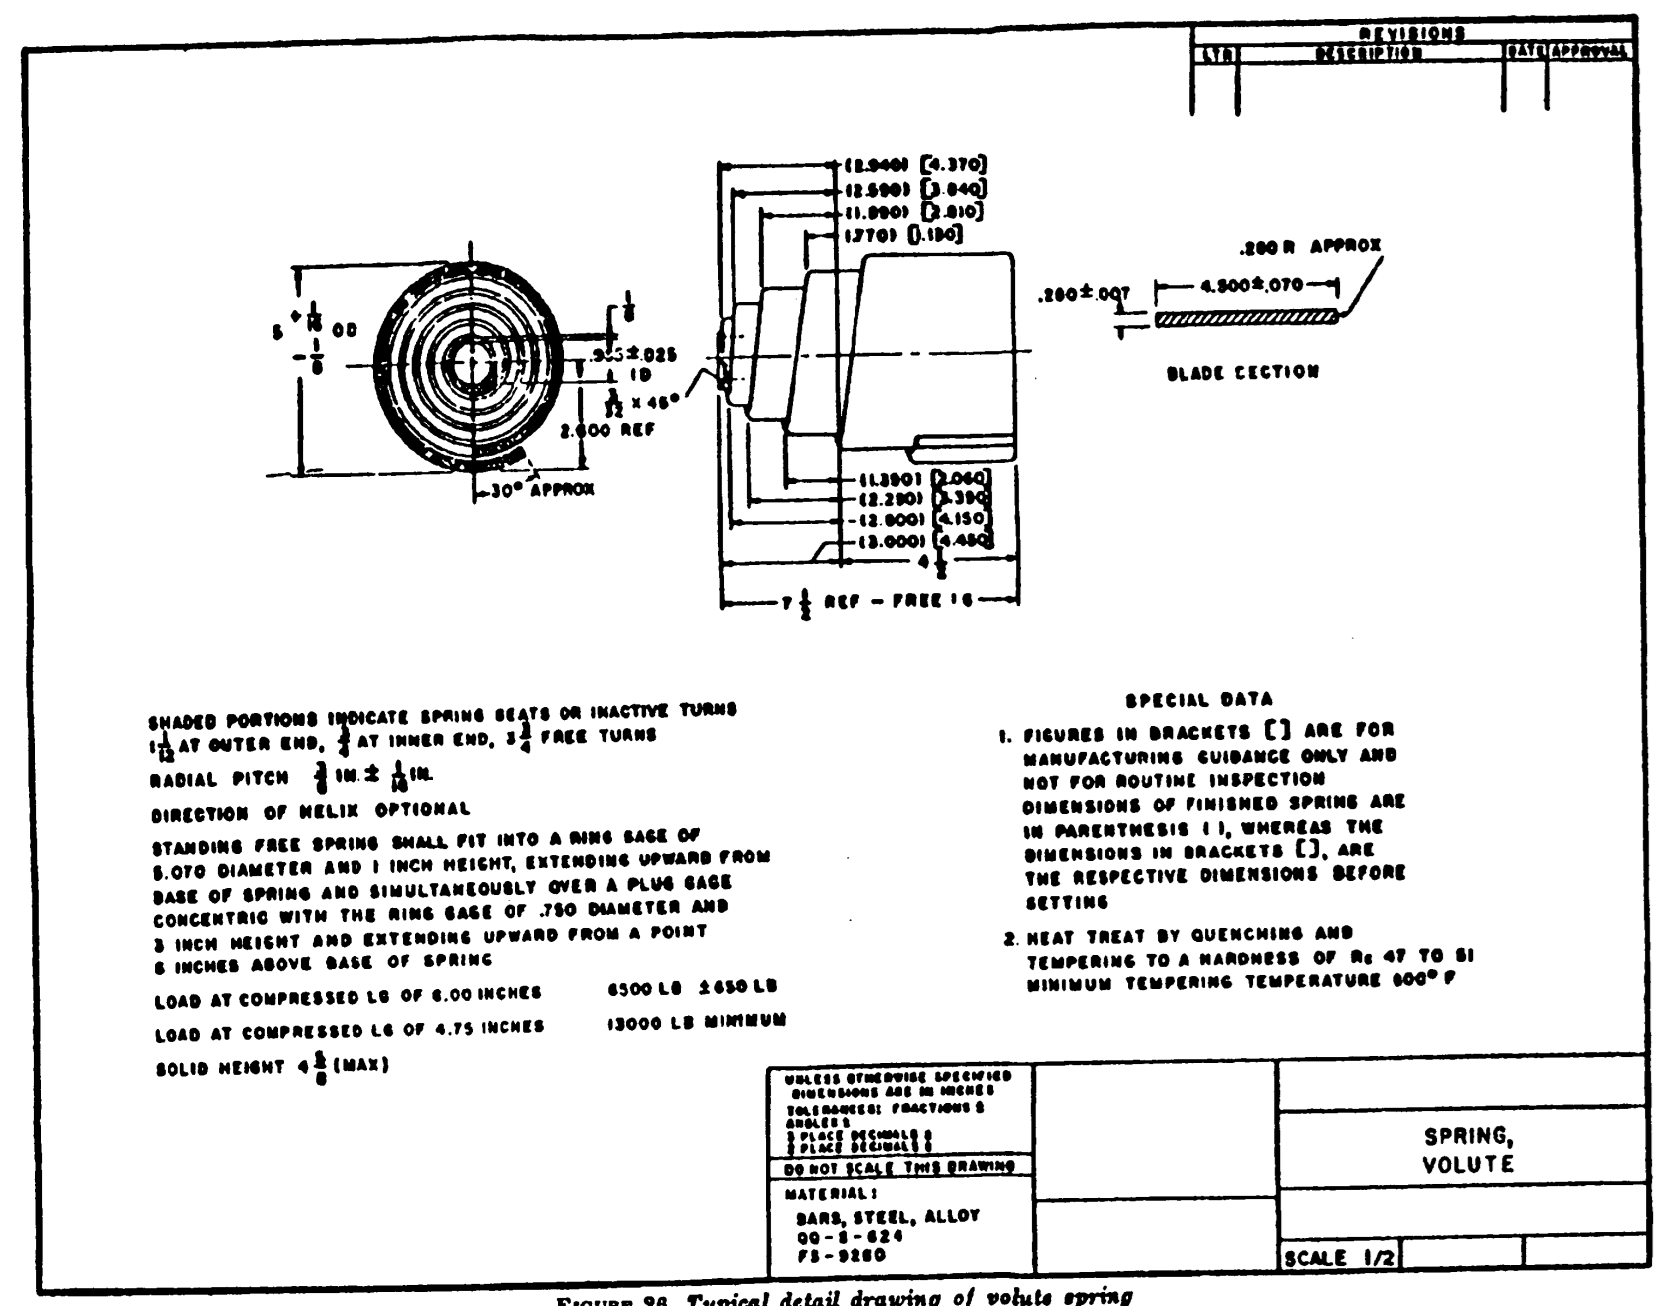
\includegraphics[width=0.8\textwidth]{milstd29a_fig26.png}
    \caption{}
    \label{fig:26}
\end{figure}

\begin{figure}[htbp] % h:here, t:top, b:bottom, p:page
    \centering
    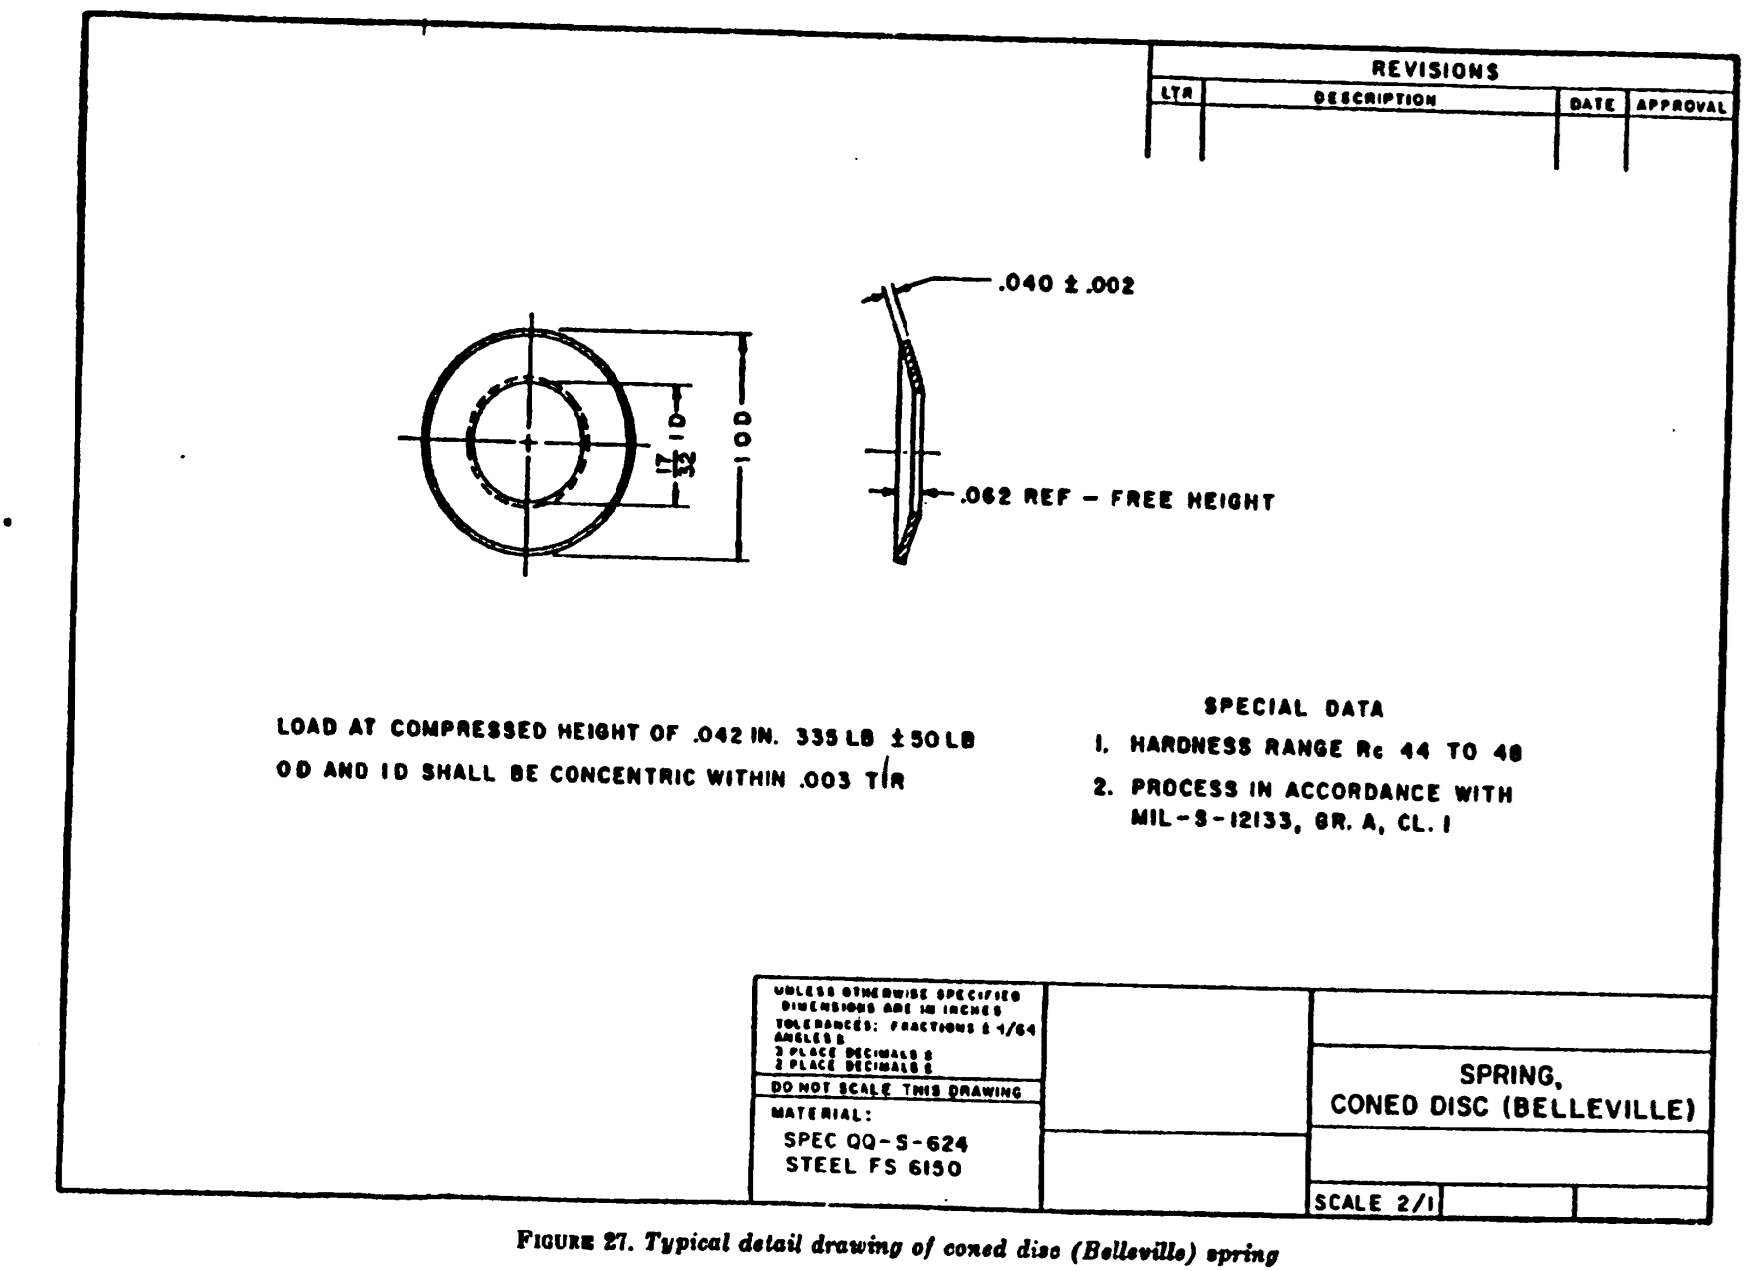
\includegraphics[width=0.8\textwidth]{milstd29a_fig27.png}
    \caption{}
    \label{fig:27}
\end{figure}

\begin{figure}[htbp] % h:here, t:top, b:bottom, p:page
    \centering
    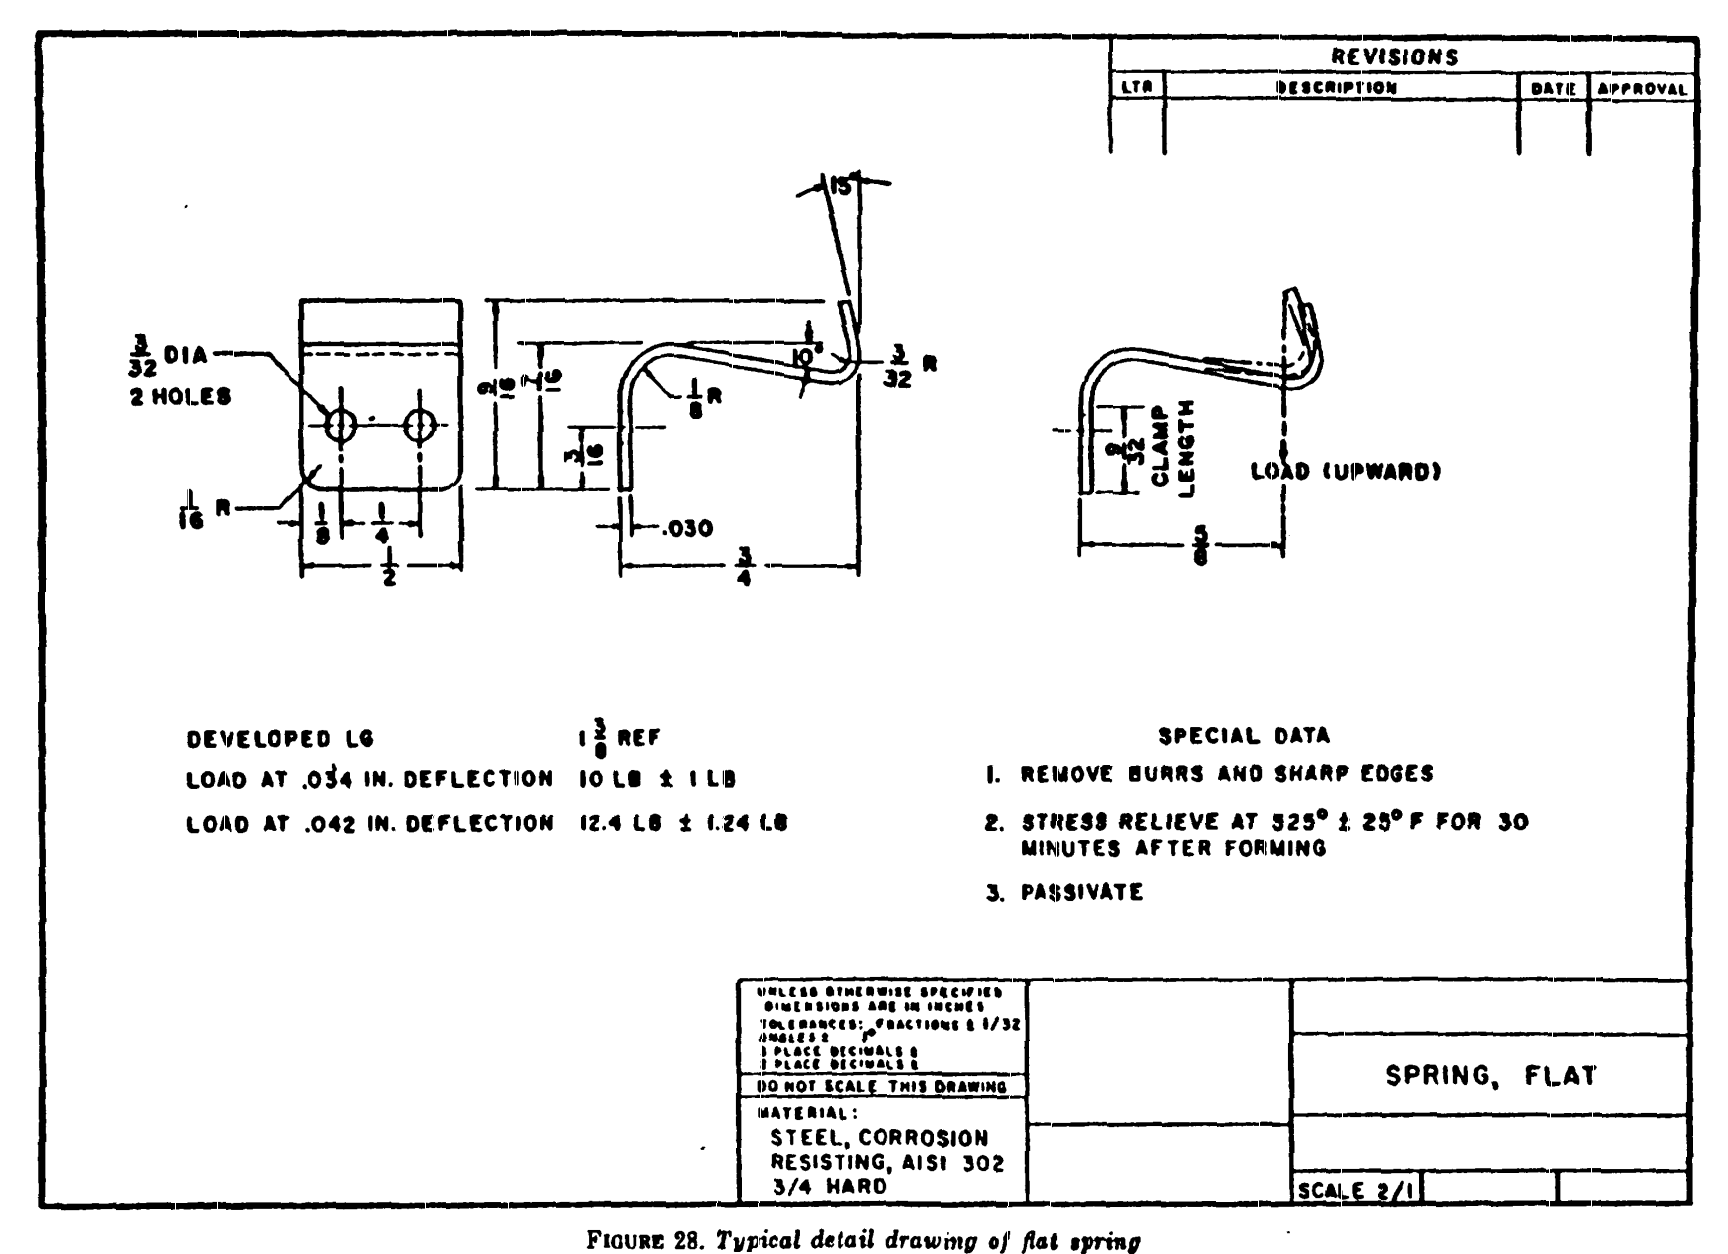
\includegraphics[width=0.8\textwidth]{milstd29a_fig28.png}
    \caption{}
    \label{fig:28}
\end{figure}

\begin{figure}[htbp] % h:here, t:top, b:bottom, p:page
    \centering
    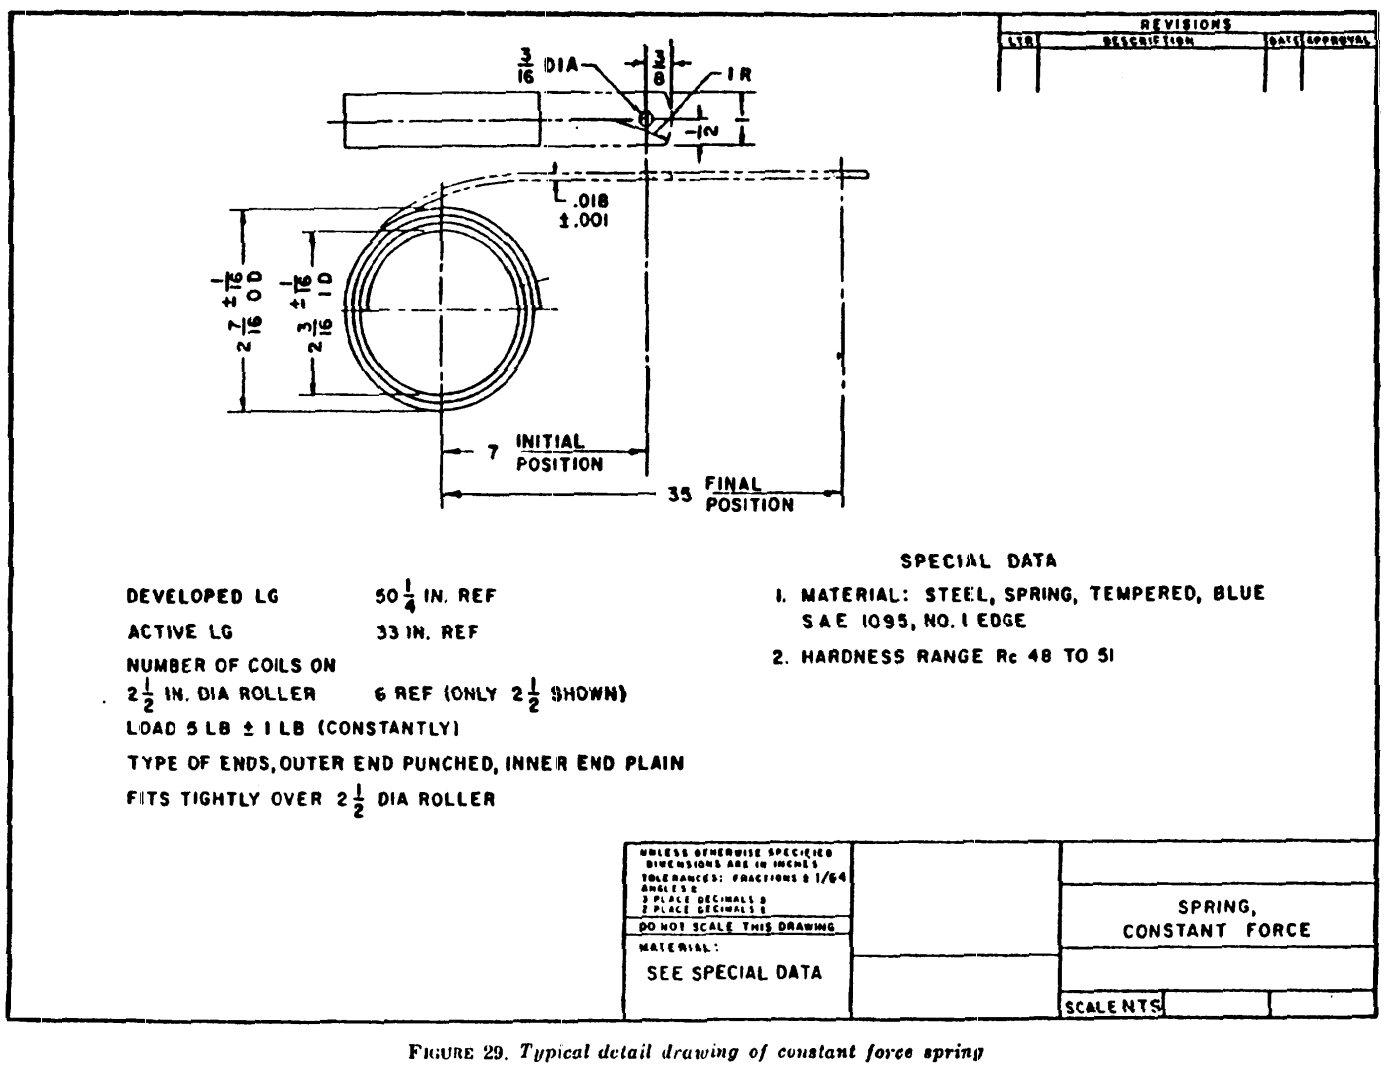
\includegraphics[width=0.8\textwidth]{milstd29a_fig29.png}
    \caption{}
    \label{fig:29}
\end{figure}

\begin{figure}[htbp] % h:here, t:top, b:bottom, p:page
    \centering
    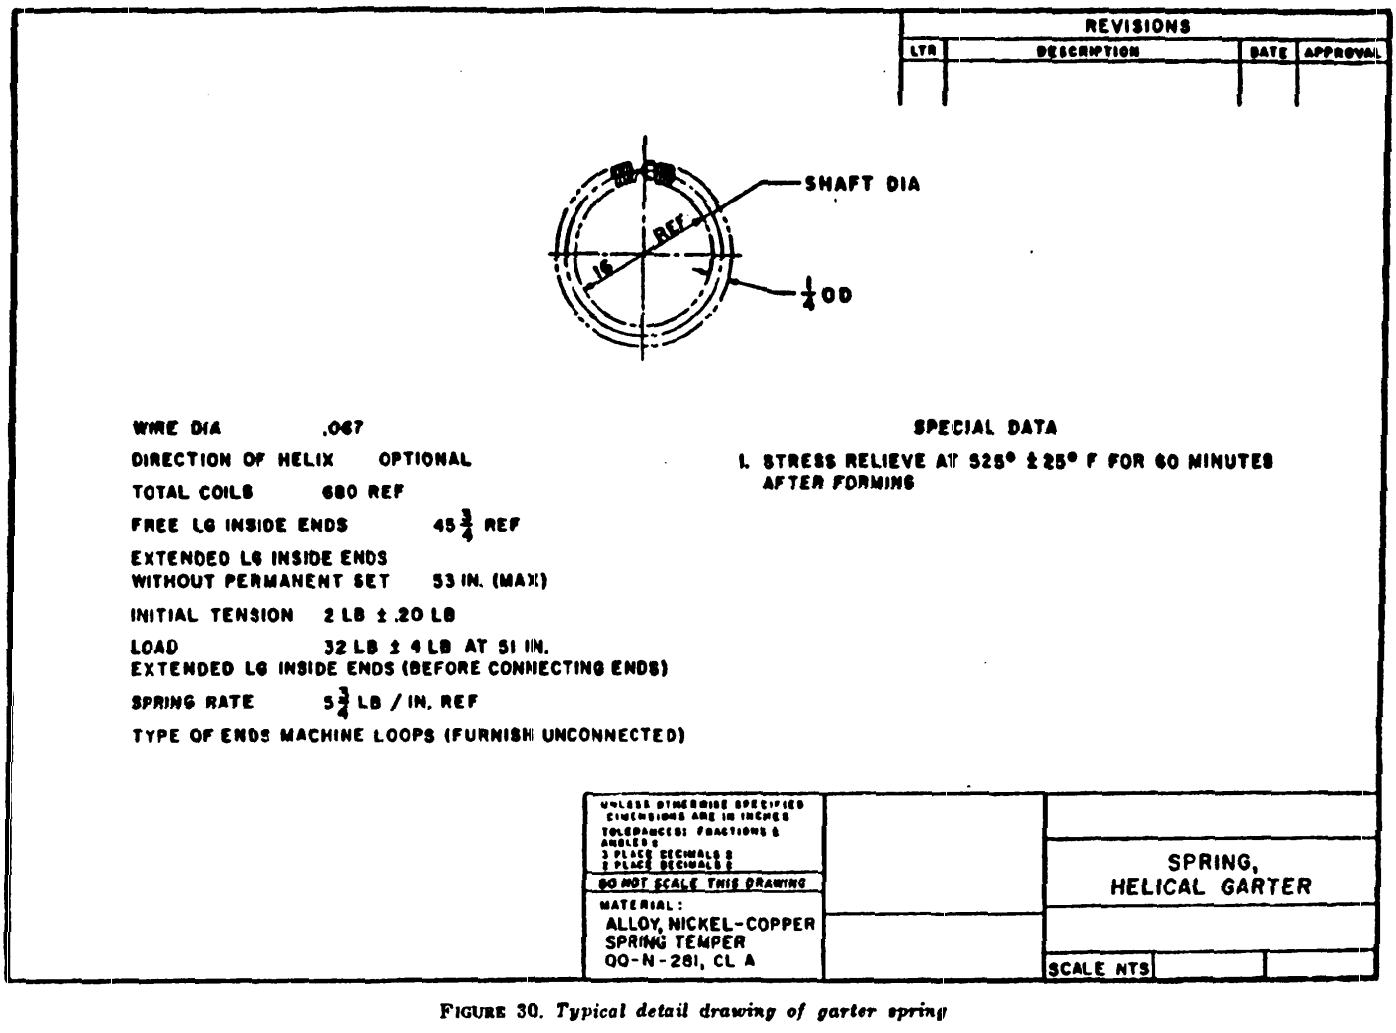
\includegraphics[width=0.8\textwidth]{milstd29a_fig30.png}
    \caption{}
    \label{fig:30}
\end{figure}


%\appendix
\clearpage
\section*{Appendix A}
\addcontentsline{toc}{section}{Appendix A}
THIS APPENDIX IS FOR THE PURPOSE OF PROVIDING GUIDANCE TO DESIGN ENGINEERS AND INCLUDES NO MANDATORY PROVISIONS.

\setcounter{section}{9} % Sets the section counter
\section{Design of Mechanical Springs} % should be section 10.
\subsection{Purpose}
The purpose of this appendix is to provide ready reference data to spring design information including data on materials, design, manufacturing processes and recommended tolerances. 
The information contained herein is intended to provide guidance to the designers of springs and not to impose restrictions in design.
\subsection{Scope}
The data contained in this appendix are sufficient for general spring design.
This appendix is divided into three sections: 

Section I— MATERIALS 

Section II — DESIGN, and 

Section III — MANUFACTURE.

% "Appendix A, Section I" heading here...
\clearpage
\section*{Appendix A, Section I}
%\centerline{\textbf{Appendix A, Section I}}

\section{Spring Materials} % section 11.
\subsection{General} % section 11.1
More than forty different steel compositions, seven corrosion resisting steels and about twenty different non-ferrous compositions are used as spring materials.
Each has some particular advantage over the others and the selection is based on seeking, in addition to other requirements, the best behavior in applications involving high stress, shock loads, elevated temperatures and corrosion resistance.
All spring wire should be used in round cross-section whenever possible as it is more readily available, less expensive, usually has higher mechanical properties and is easier to fabricate. 
Steel wire has the longest fatigue life and can withstand the highest stresses. 
Copper-base alloys have the best electrical conductivity combined with good corrosion resistance. 
Corrosion resisting steels have good resistance to moderately elevated temperatures and to corrosion. 
Nickel-base alloys have the best resistance to elevated temperatures combined with excellent corrosion resistance. 
More specific data on these materials is covered in this section. 
The SAE and AISI references and the specifications of bar in the following paragraphs represent typical compositions of metal from which springs with the specified mechanical properties can be produced.

\subsection{Sizes Available} % section 11.2
In the column headed Mechanical Properties in Paragraphs 12.2 through 17.3 are shown "Sizes Available", which lists the range of sizes usually available from warehouses or wire mills. 
For most materials both smaller and larger sizes can be obtained on special order. 
The sizes shown in Table I, Appendix A, Section I, should be used wherever possible.

\section{High Carbon Steels} % section 12.
\subsection{General}
The most commonly used of all spring materials are the high carbon spring steels. 
These materials are used in Music-Wire, Hard-Drawn Wire, Oil Tempered Wire and Valve Spring Wire. 
All are readily available in a wide variety of sizes. 
These materials should be used in preference to other materials whenever the design requirements permit their use. 
They are not usually recommended for sub zero temperature applications.

\subsection{Music Wire QQ-W-470, ASTM A228-51} % section 12.2
Music wire is the highest quality cold drawn, high carbon wire in the ferrous group.
It has exceptionally high tensile strength and uniform temper. 
It is recommended for small springs which are subjected to high stresses and suddenly applied loads.
Only round sections have high tensile strengths.
This material is not a true music wire if obtained in any sections other than round.

\begin{center}
\begin{tabular}{ r c }
\multicolumn{2}{c}{Mechanical Properties:} \\
\hline
Modulus in Tension: & E = 30 x 10$^4$ \\ 
Modulus in Torsion (Up to 0.100 in): & G = 12 x 10$^4$ \\  
Modulus in Torsion (Over 0.100 in): & G = 11.75 x 10$^4$ \\
Elastic Limit in Tension: & 65 to 75 \% of TS \\  
Elastic Limit in Torsion: & 45 to 50 \% of TS \\
Density: & 0.284 lb/in$^3$ \\
Maximum Elevated Temperature: & 250$^\circ$ F \\
Sizes Available: & 0.004 to 0.180 \\
\hline
\end{tabular}
\end{center}

\subsection{Hard Drawn Steel Wire QQ-W-428, Type II; ASTM A227-47} % section 12.3
Hard drawn steel wire is a low cost spring steel which can be used for average stress applications where accuracy of wire diameter, spring diameter and loads are not required with great precision.
Do not use in applications where long life is required.
This material can be readily electroplated.
Square section are also obtainable but at reduced tensile strengths.

\begin{center}
\begin{tabular}{ r c }
\multicolumn{2}{c}{Mechanical Properties:} \\
\hline
Modulus in Tension: & E = 30 x 10$^4$ \\  
Modulus in Torsion: & G = 11.5 x 10$^4$ \\
Elastic Limit in Tension: & 60 to 70 \% of TS \\  
Elastic Limit in Torsion: & 45 to 55 \% of TS \\
Density: & 0.284 lb/in$^3$ \\
Maximum Elevated Temperature: & 250$^\circ$ F \\
Sizes Available: & 0.028 to 0.625 in. dia \\
\hline
\end{tabular}
\end{center}

\subsection{Oil Tempered Steel Wire QQ-W-428, Type I; ASTM A229-56} % section 12.4
Oil-tempered steel wire is a general purpose spring steel of uniform quality and temper.
Because of its surface condition this material is recommended for springs where: (1) the stress requirements are not too extreme, (2) the spring is not subjected to impact or shock loading, and (3) the spring index is 5 or greater.
This material is wdiely used for mechanical products and machine tools in applications where the slight scale of the surface is not objectionable.
The scale can be removed if necessary by shot blasting.
Also obtainable in the annealed condition if desired.

\begin{center}
\begin{tabular}{ r c }
\multicolumn{2}{c}{Mechanical Properties:} \\
\hline
Modulus in Tension: & E = 28.5 x 10$^4$ \\  
Modulus in Torsion: & G = 11.2 x 10$^4$ \\
Elastic Limit in Tension: & 80 to 90 \% of TS \\  
Elastic Limit in Torsion: & 40 to 50 \% of TS \\
Rockwell Hardness & C45 - 50 less than 0.125 in. dia\\
& C42 - 48 0.126 in. to 0.250 in. dia\\
& C40 - 45 0.251 in. to 0.500 in. dia\\
Density: & 0.284 lb/in$^3$ \\
Maximum Elevated Temperature: & 350$^\circ$ F \\
Sizes Available: & 0.032 to 0.500 in. dia \\
Sizes Available in Square Section: & 1/32 to 1/2 in common fractions \\
\hline
\end{tabular}
\end{center}

\subsection{Carbon-Steel Valve Spring Quality Wire ASTM A230-47} % section 12.5
Because of the absence of scale on this material, it is suitable for use where flaking of scale would clog or otherwise injure moving parts. 
This material is recommended for springs of ininite life with an average stress range. 
This material is available in the tempered and annealed condition, but the tempered condition is most often used. 
The annealed condition should be used with subsequent hardeníng and tempering for springs with a low spring index (less than 5) or where severe forming is required.

\begin{center}
\begin{tabular}{ r c }
\multicolumn{2}{c}{Mechanical Properties:} \\
\hline
Modulus in Tension: & E = 29.5 x 10$^4$ \\  
Modulus in Torsion: & G = 11.2 x 10$^4$ \\
Elastic Limit in Tension: & 85 to 95 \% of TS \\  
Elastic Limit in Torsion: & 50 to 60 \% of TS \\
Rockwell Hardness & C45 - 50 for 0.125 in. diameter and under\\
& C42 - 48 above 0.125 in.\\
Density: & 0.284 lb/in$^3$ \\
Maximum Elevated Temperature: & 350$^\circ$ F \\
Sizes Available: & 0.093 to 0.250 in. dia \\
\hline
\end{tabular}
\end{center}

\section{Alloy Steel Wire and Bar} % Section 13.
\subsection{General} % Section 13.1
Alloy spring steels are particularly useful in applications involving high stress and where shock or impact loadings occur.
They can also withstand higher and lower temperature conditions than the carbon spring Steels. 
All these alloys are generally used in the oil tempered or pre-hardened condition. 
They also are obtainable in the annealed condition for springs that have sharp bends or small spring indexes such as 5 or less.

\subsection{Chrome-Vanadium Alloy Steel Wire \& Bar ASTM A231-41 (Wire); QQ-S-624 FS 6150; A60-49 (Bars); ASTM A232-47 (Wire); QQ-W-412, Comp 1 (Wire)} % Section 13.2

Chrome-Vanadium alloy steel wire will withstand higher stresses than Oil-tempered steel wire, but not as high as music wire. 
This material is recommended for springs which are subjected to shock by impact or suddenly applied loads, and for springs which are subjected to a large number of stress cycles. 
This material is frequently used for die springs. 
It is especially useful when annealed round wire is flattened into rectangular section with round edges. 
Die springs made from such sections are hardened and tempered after coiling and then shotpeened to increase their endurance limit. 
Hot rolled bars in heavy sections are also used for hot rolled springs and torsion bars.

Mechanical Properties:

Modulus;

In tension E=29.5 x 10$^4$

In torsion

G=11.2 x 10$^4$

Elastic Limit;

Tension=88 to 93\% of TS

Torsion=65 to 75\% of TS

Rockwell Hardness=C45-50

Density=.284 lb/in.

Maximum elevated temperature

425$^\circ$ F

Sizes Available:

.032 to .375 in. dia in the tempered or annealed condition; 7/16 to 2 in. dia in bars for hot rolled springs.
Square sections in common fractional sizes are also obtainable.

\subsection{Silico-Manganese Alloy Steel Bar SAE 9260 \& ASTM A59-49 (Bar)} % Section 13.3
This alloy steel has frequently been used as a less expensive substitute or alternate for chrome-vanadium. 
It does not have mechanical properties quite as high as other alloy steels. 
This alloy is obtainable in the oil-tempered, and in the annealed conditions in hot rolled bars. 
Heavy flat sections have been used for leaf springs and torsion bars.

Mechanical Properties:

Modulus:

In tension

E = 29.5 x 10$^4$

In torsion

G = 112 x 10$^4$

Elastic Limit;

In tension = 78 to 86\% of TS

In torsion = 55 to 65\% of TS

Rockwell Hardness = C44 to 48

Density=284 lb/in.

Sizes Available: 7/16 to 2 in. dia bars

\subsection{Chrome-Silicon Alloy Steel Wire QQ-W-412, Comp 2, Type II; ASTM A401-58} % Section 13.4
This alloy steel is especially suited for highly stressed springs subjected to shock or impact loading such as recoil springs in anti-aircraft guns and for moderately elevated temperatures. 
It may be obtained in the oil-tempered condition, but has most often been used in the annealed condition and then hardened and tempered to quite high hardness after coiling.

Mechanical Properties:

Modulus;

In tension:

In torsion:

Elastic Limit:

Rockwell Hardness = C50 to C53

Density = 0.284 lb/in$^3$

Maximum elevated temperature 475$^\circ$

Sizes Available: 0.032 to 0.375 in. dia wire.

\clearpage
\section{Corrosion Resisting Steel Wire} % Section 14.
\subsection{General} % Section 14.1
Corrosion resisting steels are especially useful in applications involving corrosion and high temperatures.
The 300 series "18-8" chromium-nickel austenitic types are usually used up to about 3/16 inch diameter and the 400 series chromium martensitic types for larger sizes. 
The 300 series "18-8" types are hard-drawn to high tensile strengths and cannot be hardened by heat treatment.
The 400 series martensitic types are usually used in the annealed condition and then hardened and tempered after coiling.
The 300 series are non-magnetic in the fully annealed condition only, hard drawing to obtain spring qualities cause some magnetic ability which cannot be totally removed. 
The 400 series are magnetic and should not be used at sub zero temperatures.
Passivating or immunizing by dipping in a 20 to 40\% solution of nitric acid after fabrication is desirable for flat strip, but is frequently omitted on springs made of round wire.

\subsection{Corrosion-Resisting Steel Wire QQ-W423, Composition Type FS302 Condition B; AISI 302; SAE 30302; ASTM A313-55} % Section 14.2
This is a general purpose corrosion resisting material. 
Its spring properties are developed by cold working only. 
This material has higher tensile strengths than FS 304 and FS 316 but does not possess quite as good corrosíon resisting properties.
It is slightly magnetic in the spring temper, has low creep and resists relaxation at elevated temperatures. 
This material is also available in strip form for flat springs.



\subsection{Corrosion-Resisting Steel Wire QQ-W-423, Composition Type FS304, Condition B; AISI 304; SAE 30304} % Section 14.3
(yet to be transcribed)

\subsection{Type FS316} % Section 14.4
(yet to be transcribed)

\subsection{Corrosion Resisting Steel Wire 17-7 PH} % Section 14.5
This new type of corrosion resisting steel is of the precipitation hardening type. 
It is obtainable in the annealed condition, but it is most often used in the cold worked condition and then precipitation hardened at 900$^\circ$ F for 1 hour.
It then has tensile strengths higher than FS 302 and in some smaller sizes the tensile strength is equal to that of music wire.

\begin{center}
\begin{tabular}{ r c }
\multicolumn{2}{c}{Mechanical Properties:} \\
\hline
Modulus in Tension: & E = 29.5 x 10$^4$ \\  
Modulus in Torsion: & G = 11 x 10$^4$ \\
Elastic Limit in Tension: & 75 to 80 \% of TS \\  
Elastic Limit in Torsion: & 55 to 60 \% of TS \\
Rockwell Hardness: & C47 - 50 after hardening \\
Density: & 0.277 lb/in$^3$ \\
%Maximum Elevated Temperature: & 250$^\circ$ F \\
Sizes Available: & 0.030 to 0.375 in. dia \\
\hline
\end{tabular}
\end{center}

\subsection{Corrosion-Resisting Steel Wire QQ-W-423, Composition Type FS 420; AISI 420; SAE 51420} % Section 14.6
(yet to be transcribed)

\subsection{Corrosion-Resisting Steel Wire AISI 431; SAE 51431} % Section 14.7
This new type corrosion resisting steel is first hardened and tempered and then cold drawn. 
This combination produces bright clean wire with high tensile strengths nearly as high as music wire, but its corrosion resistance is not quite equal to FS 302. 
The hardened wire is magnetic and finds many uses for springs subjected to high stresses. 
Flat strip is also available.

\begin{center}
\begin{tabular}{ r c }
\multicolumn{2}{c}{Mechanical Properties:} \\
\hline
Modulus in Tension: & E = 30 x 10$^4$ \\  
Modulus in Torsion: & G = 11.5 x 10$^4$ \\
Elastic Limit in Tension: & 72 to 75 \% of TS \\  
Elastic Limit in Torsion: & 50 to 55 \% of TS \\
Rockwell Hardness: & C47 - 51 \\
Density: & 0.280 lb/in$^3$ \\
%Maximum Elevated Temperature: & 250$^\circ$ F \\
Sizes Available: & 0.050 to 0.312 in. dia \\
\hline
\end{tabular}
\end{center}

\clearpage
\section{Copper Base Alloys} % Section 15.
\subsection{General} % Section 15.1
Copper-base alloys combine good electrical properties with excellent corrosion resistance. 
Although more expensive than steel they find many use in electrical components and are excellent at sub zero temperature applications. 
All are non-magnetic.

\subsection{Spring Brass Wire QQ-W-321, Composition B, Spring Temper; ASTM B134-52, Alloy 6; SAE 80A} % Section 15.2
Spring brass is recommended for use where high electrical conductivity, excellent corrosion resistance, ease of forming, low cost, and repeated flexure at low stress and low temperatures are required.
Spring brass is non-magnetic.
It is not recommended for applications where stress is severe. 
It is also available in flat strip.
\begin{center}
\begin{tabular}{ r c }
\multicolumn{2}{c}{Mechanical Properties:} \\
\hline
Modulus in Tension: & E = 15 x 10$^4$ \\  
Modulus in Torsion: & G = 5.0 x 10$^4$ \\
Elastic Limit in Tension: & 75 to 80 \% of TS \\  
Elastic Limit in Torsion: & 45 to 50 \% of TS \\
Rockwell Hardness: & B89 - 95 \\
Density: & 0.308 lb/in$^3$ \\
Maximum Elevated Temperature: & 150$^\circ$ F \\
Sizes Available: & 0.005 to 0.500 in. dia \\
\hline
\end{tabular}
\end{center}

\subsection{Phosphor Bronze Wire QQ-W-401; ASTM B159-58, Alloy A; SAE 81} % Section 15.3
Phosphor bronze is used for electrical conductivity, ability to resist corrosion, and non-magnetic properties.
It has good bending and forming properties and the ability to withstand repeated flexures.
This is the most popular of the copper-base non-ferrous alloys.
It is also available in flat strip for electrical contact fingers.
Superfine grain structure withstands quite high stresses and has long endurance to repeated flexure.
\begin{center}
\begin{tabular}{ r c }
\multicolumn{2}{c}{Mechanical Properties:} \\
\hline
Modulus in Tension: & E = 15 x 10$^4$ \\  
Modulus in Torsion: & G = 6.0 x 10$^4$ \\
Elastic Limit in Tension: & 75 to 80 \% of TS \\  
Elastic Limit in Torsion: & 45 to 50 \% of TS \\
Rockwell Hardness: & B90 - 97 \\
Density: & 0.320 lb/in$^3$ \\
Maximum Elevated Temperature: & 212$^\circ$ F \\
Sizes Available: & 0.005 to 0.500 in. dia \\
\hline
\end{tabular}
\end{center}

\clearpage
\subsection{Beryllium Copper Wire QQ-C-530; ASTM B197-52} % Section 15.4
Beryllium copper is a precipitation hardening non-magnetic material with good electrical conductivity and corrosion resistance. 
It is non-magnetic and has high elastic and fatigue strength, and low drift and hysteresis.
This material can be severely formed in the annealed condition.
Following forming, beryllium copper is precipitation hardened at 600$^\circ$ F for 2 hours.
Pretempered wire is also useful for many applications where the stresses are not too high.
Flat strip is also available.
\begin{center}
\begin{tabular}{ r c }
\multicolumn{2}{c}{Mechanical Properties:} \\
\hline
Modulus in Tension: & E = 19 x 10$^4$ \\  
Modulus in Torsion: & G = 7.3 x 10$^4$ \\
Elastic Limit in Tension: & 75 \% of TS \\  
Elastic Limit in Torsion: & 50 to 55 \% of TS \\
Rockwell Hardness: & C37 - 41 \\
Density: & 0.298 lb/in$^3$ \\
Maximum Elevated Temperature: & 300$^\circ$ F \\
Sizes Available: & 0.005 to 0.500 in. dia \\
\hline
\end{tabular}
\end{center}

\clearpage
\section{Nickel Base Alloys} % Section 16.
\subsection{General} % Section 16.1
Nickel-base alloys have excellent corrosion resistance combined with ability to withstand both elevated and below zero temperature applications.
Also, their non-magnetic characteristic is important for such devices as gyroscopes, chronoscopes and indicating instruments.
These materials have high electrical resistance and should not be used for conductors of electrical current.

\subsection{Nickel Copper Alloy, QQ-N-281, Class A, Spring Temper (Monel)} % Section 16.2
Monel is recommended for use at elevated temperatures where corrsive conditions exist. 
It retains its corrosive resistance properties at relatively high temperatures. 
This material has good resistance to sea water attack.

Mechanical Properties:

Modulus;


E = 26.0 x 10

In torsion


Elastic Limit;

Tension=65 to 70\% of TS


Density =.319 lb/in.

Maximum elevated temperature

400$^\circ$ F (450$^\circ$ F-for short periods)

Sizes Available:

.005 to 250 in. dia full hard, over .250 at lower hardness.


\subsection{Nickel-Copper-Aluminum Alloy, Wrought, QQ-N-286, Class A (K-Monel)} % Section 16.3
K-Monel is a precipitation hardening alloy with excellent resistance to both corrosion and moderately elevated temperatures. 
It is usually used in larger sizes than Monel, as it can be formed in the cold drawn condition and then heat treated for hardening purposes. 
The mechanical properties are for the spring temper, age hardened condition. 
This alloy is non-magnetic.
\begin{center}
\begin{tabular}{ r c }
\multicolumn{2}{c}{Mechanical Properties:} \\
\hline
Modulus in Tension: & E = 26.0 x 10$^4$ \\  
Modulus in Torsion: & G = 9.5 x 10$^4$ \\
Elastic Limit in Tension: & 65 to 70 \% of TS \\  
Elastic Limit in Torsion: & 38 to 42 \% of TS \\

%Rockwell Hardness: & C47 - 51 \\
Density: & 0.305 lb/in$^3$ \\
Maximum Elevated Temperature: & 450$^\circ$ F (500$^\circ$ F for short periods) \\
Sizes Available: & 0.005 to 0.563 in. dia for cold wound springs \\
& 3/8 in. dia and over for hot wound springs \\
\hline
\end{tabular}
\end{center}

\subsection{Wire: Nickel-Chromium-Iron Alloy, QQ-W-390, Condition C (Inconel)} % Section 16.4
Inconel is recommended for springs requiring: 
(1) the retention of spring properties at relatively high temperatures, 
(2) corrosion resistance, 
(3) low magnetic permeability. 
This is one of the most popular of the nickel-base alloy group. 
It is cold drawn and cannot be hardened by heat treatment. 
Wire diameters up to 1/4 inch are most often used. 
This alloy is non-magnetic.

Mechanical Properties:

Modulus;

In tension

E=81 x 10 at 70$^\circ$ F.

29.5 x 10 at 40$^\circ$ F
29.2 x 10 at 500$^\circ$ F.
28.7 x 10 at 600$^\circ$ F.
28.2 x 10 at 700$^\circ$ F.
28.0 x 10 at 750$^\circ$ F.

In torsion

G=11.2 x 10 at 70$^\circ$ F.

10.8 x 10 at 400$^\circ$ F.
10.5 x 10 at 500$^\circ$ F.
10.2 x 10 at 600$^\circ$ F.
10.0 x 10 at 700$^\circ$ F.
9.8 x 10 at 750$^\circ$ F.

Elastic Limit;

In tension =65 to 70\% of TS

In torsion = 40 to 45\% of TS

TS=185,000 up to .057 in dia incl

175,000 over .057 in. to .114 in dia incl

170,000 over .114 in. to .229 in. dia incl

165,000 over 229 in. to .329 in. dia incl

160,000 over .329 in. to .375 in. dia incl

155,000 over .375 in. to .500 in dia incl

140,000 over .500 in. to .563 in. dia incl

Density.304 lb/in.

Maximum elevated temperature

650$^\circ$ F. (750$^\circ$ F. for short periods)

Sizes Available:
.010 to .1875 in. dia full hard, over .1875 at lower hardness.


\subsection{Nickel Alloy Spring Wire, AMS 5698 for No. 1 Temper; AMS 5699 for Spring Temper (Inconel X)} % Section 16.5
Inconel-X is a precipitation hardening material with high corrosion resistance and oxydization resistance at elevated temperatures. 
To make optimum use of this material, it is recommended that it be used in applications where the temperature is from 650 to 1150$^\circ$ F. 
For applications below 650$^\circ$ F the use of other materials is recommended. 
Neither cold setting nor shot peening should be specified on product drawing, when springs are intended to be operating
within the recommended temperatures (650 to 1150$^\circ$ F) due to the adverse effect of pre-stressing on inittal retaxation and the rate of relaxation under heat and stress.. 
Large diameter bars can be hot coiled, and this is often done for 3s in dia and larger sizes depending upon the spring index.
This non-magnetic alloy can also be used at sub-zero temperatures. 
The mechanical properties are for the tempers indicated after age hardening. 
For sub zero to 700$^\circ$ F applications, use spring temper stock and heat 1200$^\circ$ F for 4 hours, after coiling. 
For 700 to 1000$^\circ$ F applications, use No. 1 temper (or hot fmished stock) and heat 1350$^\circ$ F for 16 hours, after coiling. 
For 1000 to 1200$^\circ$ F applications, use spring temper stock and heat 2100$^\circ$ F for 2 hours, air cool, then 1550$^\circ$ F for 24 hours, air cool and 1300$^\circ$ F for 20 hours and air cool, after coiling.
\begin{center}
\begin{tabular}{ r c }
\multicolumn{2}{c}{Mechanical Properties:} \\
\hline
Modulus in Tension: & E = 31 x 10$^4$ at 70$^\circ$ F \\  
& E = 28.1 x 10$^4$ at 700$^\circ$ F \\ 

& E = 25.5 x 10$^4$ at 1200$^\circ$ F \\ 

Modulus in Torsion: & G = 11.2 x 10$^4$ at 70$^\circ$ F \\
& G = 10.0 x 10$^4$ at 700$^\circ$ F \\

Elastic Limit in Tension: & 85 to 90 \% of TS \\  
Elastic Limit in Torsion: & 65 to 75 \% of TS \\
Tensile Strength: & For No. 1 temper: \\
& 244,000 to 305,000 for sizes under .032 in. \\
& 214,000 to 240,000 for sizes over .032 in. \\
& For spring temper: \\
Rockwell Hardness: & C46 - 49 \\
Density: & 0.298 lb/in$^3$ \\
Maximum Elevated Temperature: & 1150 to 1200$^\circ$ F at low stresses\\
Sizes Available: & 0.005 to 0.062 in. thickness, others on special order \\
\hline
\end{tabular}
\end{center}

\clearpage
\section{Steel Strip High Carbon} % Section 17.
\subsection{General} % Section 17.1
Several types of flat cold rolled steel strip with different ranges of carbon content, tempers, finishes and edges are obtainable, but only two types are readily available.
These two types are used for over 95 per cent of all applications reqairing steel strip. 
Thin sections of high hardness (over Rockwell "C" 43) are highly susceptible to hydrogen embrittlement resulting from electroplating or pickling operations. 
These materials are used for mainsprings in clocks and timing devices; for constant force springs, clips and stampings. 
For general information see Spec. MIL-S-17919.

\subsection{Steel Strip, High Carbon SAE 1074; MIL-S-17919 Matl. No. 1 \& 4} % Section 17.2
This type of material is usually called "cold rolled blue tempered spring steel". 
It is slit to desired widths and the edges can be squared or rounded as desired. 
The material obtained in the hardened conditions is widely used for flat springs, spiral, clock and motor springs. 
It is also available in the annealed condition for use in automatic equipment and where severe forming operations are required, after which it is hardened and tempered.
\begin{center}
\begin{tabular}{ r c }
\multicolumn{2}{c}{Mechanical Properties:} \\
\hline
Modulus in Tension: & E = 30 x 10$^4$ \\  
Modulus in Torsion: & G = 11.5 x 10$^4$ \\
Elastic Limit in Tension: & 85 to 90 \% of TS \\  
Elastic Limit in Torsion: & 65 to 75 \% of TS \\
Tensile Strength: & 244,000 to 305,000 for sizes under .032 in. \\
& 214,000 to 240,000 for sizes over .032 in. \\
Rockwell Hardness: & C46 - 49 \\
Density: & 0.284 lb/in$^3$ \\
Maximum Elevated Temperature: & 350$^\circ$ F \\
Sizes Available: & 0.005 to 0.062 in. thickness, others on special order \\
\hline
\end{tabular}
\end{center}

\subsection{Steel Strip, High Carbon SAE 1095; MIL-S-17919 Matl. No. 1 \& 2} % Section 17.3
This type of material, usually called "cold rolled blue tempered and polished clock spring steel", is widely used in clocks and motor springs because it can withstand higher stresses than SAE 1074. 
It is slit to widths desired and the edges are usually made square or rounded. 
It is generally obtained in the hardened condition, but annealed material can be obtained.
\begin{center}
\begin{tabular}{ r c }
\multicolumn{2}{c}{Mechanical Properties:} \\
\hline
\multicolumn{2}{c}{The same as SAE 1074 but the tensile strengths are about 5 per cent higher.} \\
%Modulus in Tension: & E = 30 x 10$^4$ \\  
%Modulus in Torsion: & G = 11.5 x 10$^4$ \\
%Elastic Limit in Tension: & 72 to 75 \% of TS \\  
%Elastic Limit in Torsion: & 50 to 55 \% of TS \\
Rockwell Hardness: & C48 - 51 \\
%Density: & 0.280 lb/in$^3$ \\
%Maximum Elevated Temperature: & 250$^\circ$ F \\
%Sizes Available: & 0.050 to 0.312 in. dia \\
\hline
\end{tabular}
\end{center}


% Page 57:
\clearpage
Table I. Preferred sizes for spring materials wire diameters, strip thickness and bars

% Table goes here...
\begin{figure}[htbp] % h:here, t:top, b:bottom, p:page
    \centering
    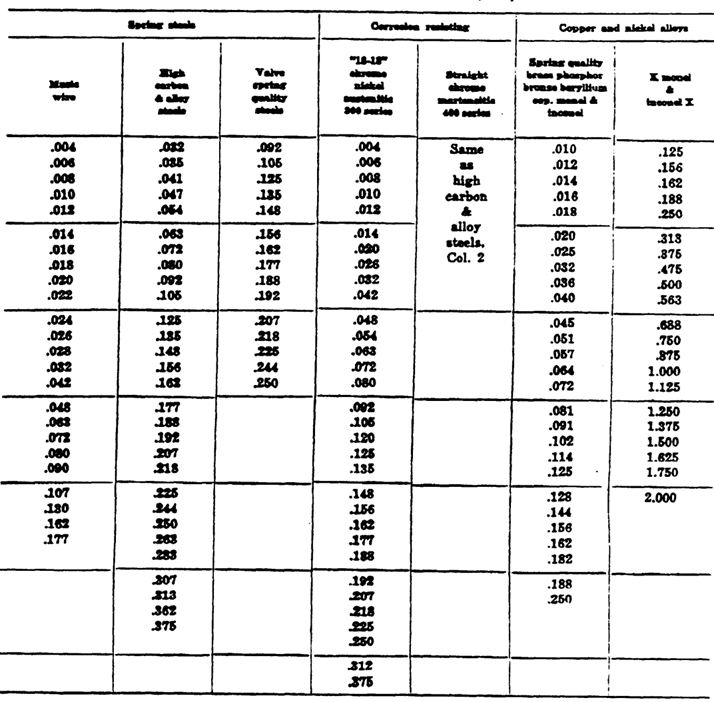
\includegraphics[width=0.9\textwidth]{milstd29a_table_i.png}
    %\caption{}
    %\label{fig:table_i}
\end{figure}

Note 1. Square sizes of wire and bars are obtainable in preferred fractional sizes as follows: 1/32, 1/16, 3/32, 1/8, 5/32, 3/16, 7/32, 1/4, 9/32, 5/16, 3/8, 7/16, 1/2, 9/16, 5/8, 11/16, 3/4, 13/16, 7/8, 15/16, 1, 1 1/16, 1 1/8, 1 3/16, 1 1/4,  1 5/16, 1 3/8, 1 1/2, 1 5/8, 1 3/4, 1 7/8 and 2 in.

Note 2. Music wire and Valve spring quality wire are available in round sections only.

Note 3. Music wire is drawn to American Steel Wire \& Music Wire Gage and to special gages. 
Steel wire is drawn to U.S. Steel Wire Gage (same as Washburn \& Moen Gage). 
Copper and Nickel Alloys are drawn to the American Wire Gage (same as Brown \& Sharpe Gage).



\clearpage
% Page 58:
\section*{Appendix A, Section II}
\setcounter{section}{19} % Sets the section counter
\section{Spring Design} % should be section 20.
\subsection{General} % should be section 20.1
The proper design of springs requires an understanding of

1 - spring materials,

2 - design formulas and stress analysis,

3 - manufacture.

\noindent Various aids to designers are available including special spring slide rules, tables of constants, curves, charts and nomographs.
All are helpful, but an understanding of the basic fundamental formulas and experience in their use is essential to good design. 
Except for a few sizes of valve and die springs, there are very few springs manufactured for stock because of the infinite variety of characteristics involved.
Utmost care in their design and manufacture and thorough analysis of service conditions are required for satisfactory performance.
\subsubsection{Purpose} % should be section 20.1.1
The purpose of this section is to describe the design methods used for each type of spring commonly used.

\subsubsection{Scope} % should be section 20.1.2
The data in this appendix are sufficient for general design purposes, and is not intended to include information for unusual designs or seldom used types of springs.

\subsubsection{Abbreviations and Symbols} % should be section 20.1.3
The following abbreviations and symbols are used throughout the appendix, unless otherwise noted:

$A$ = constant, for rectangular wire.

$B$ = constant, for rectangular wire.

$b$ = breadth or width, in.

$C$ = spring index = $D/d$.

$CL$ = compressed length, in.

$D$ = mean coil diameter, in.

$d$ = diameter of wire or side of square, in.

$E$ = modulus of elasticity in tension, psi.

$F$ = deflection, for $N$ coils with load $P$, in.

$F^o$ = deflection, for $N$ coils, rotary, deg.

$FL$ = free length, unloaded spring, in.

$f$ = deflection, for one active coil, in., at load $P$.

$G$ = modulus of elasticity in torsion, psi.

$ID$ = inside diameter, in.

in. = inch.

$K$ = curvature stress-correction factor 

$L$ = active length subject to deflection, in.

$l$ = length, in.

lb = pound

$M$ = bending moment, in. lb.

$N$ = total active coils

$n'$ = vibration per minute.

$OD$ = outside diameter, in.

$P$ = load, lb.

$P_1$ = applied load, lb (also $P_2$, etc.)

$p$ = pitch, in.

psi = pounds per square inch.

$R$ = distance from load to central axis, in.

$r$ = spring rate, load per in, lb/in.

$r_t$ = spring rate, inch lbs per deg. (Torsion springs).

$S_b$ = stress, bending, psi.

$S_t$ = stress, torsional, psi.

$S_it$ = stress, torsinal, due to intial tension, psi.

$SH$ = solid height, in. (or SL = solid length).

$s$ = height, load is dropped, in.

$T$ = torque = $P$ x $R$, lb. in.

$TC$ = total coils.

$t$ = thickness, in.

$U$ = number of revolutions = $F^o$ / 360

$W$ = weight, lb (also applied dynamic load).

x = multiplied by

$Y$ = constant, for coned disc (Belleville) springs.

$Z_1$ = constant, for coned disc (Belleville) springs.

$Z_2$ = constant, for coned disc (Belleville) springs.

$\alpha$ = alpha, angle of movement, deg.

$\pi$ = pi, 3.1416, in.

$\sigma$ = sigma, Poisson's ratio, 0.3 for steel

\setcounter{section}{20} % Sets the section counter
\section{Compression Springs} % should be section 21.
\subsection{Design Formulas} % should be section 21.1
The design formulas in Table II are used in the design of helical compression and extention springs.
Note that the same formulas apply to both types of springs. 
The formulas in Table III are for determining compression spring dimensions only.

\subsection{Compression Spring Ends} % should be section 21.2
Figure 3 illustrates the types of ends on compression springs. 
Their characteristics follow:

(a) Open Ends Not Ground; 

also called Plain Ends, has the largest eccentricity of loading. 
These are used only when accuracy of loads is not important. 
This type is seldom used because such springs tangle severely during shipping.

(b) Closed Ends Not Ground; 

also called squared ends, cost approximately the same as open end type and have less eccentricity.
This type is often used on light wire springs under 1/32 in. dia wire and for heavier wire where the index exceeds 13.

(c) Open Ends Ground; 

also called Plain Ends Ground, are seldom used as they cost about the same as the closed ends ground, but have high eccentricity of loading and tangle during shipping. 
They are sometimes used where the solid height iS very limited and it is necessary to have as many active coils as possible in the least space.

(d) Closed Ends Ground; 

also called Squared and Ground, is the most popular type as it provides a level seat and reduces the tendency to buckle. 
This is the most expensive type and should be avoided for springs made from very light wire. 
Each end coil is ground for 270$^o$ plus or minus 30$^o$.

\subsection{Diameter Changes In Compression Springs} % Section 21.3
When a helical compression spring is compressed an increase in the outside diameter occurs because the angularity of the coils changes so that it is nearly at a right angle to the axis. 
The outside diameter, when the spring is compressed solid, can be obtained from the following formula:
$$ OD_c = \sqrt{D + \frac{p^2 - d^2}{\pi^2}} + d$$
In which:

$OD_c$ = outside diameter at solid length

$p$ = pitch, at free length

$D$ = mean coild diameter at free length

$d$ = wire diameter

\subsection{Buckling} % Section 21.4
Compression springs having a free length greater than four (4) times their mean diameter become critical in lateral stability. 
When deflected beyond a certain percentage of the free length a spring will buckle. 
Figure 31 shows the maximum deflection which may be expected without buckling if the ends of the spring are closed and ground. 
Buckling can be reduced, space permitting, by a redesign using a heavier size wire and increasing the diameter of the coil. Buckling causes an undesirable reduction of the load and may cause early spring failure. 
If properly guided in a cylinder or over a rod, buckling can be reduced, although friction against the guiding member will affect the load and shorten the spring life.

\subsection{Direction of Helix} % Section 21.5
Unless functional requirement dictate a definite direction, the helix of compression and extension springs should be specified as optional. 
To prevent intermeshing of coils when springs operate one inside the other (see Figure 33), the helixes should be specified as opposite hand. 
For the same reason, springs which operate to slide freely over screw threads should have the helix specified opposite to that of the screw threads, but when a spring screws onto the threads of a screw or bolt, it should have the same helix as that of the screw or bolt.

\subsection{Natural Frequency, Vibration and Surge} % Section 21.6

\subsection{Impact} % Section 21.7

\subsection{Spring Nests} % Section 21.8

\subsection{Compression Spring Used As An Extension Spring} % Section 21.9

\subsection{Spring Index (D/d)} % Section 21.10

\subsection{Curvature Stress-Correction Factor (K)} % Section 21.11

In designing a spring it should be borne in mind that the total stress, as determined by this method, should not be used in calculating the defection or number of coils. 
The torsional stress $S_t = PD/0.393 d^3$ or$ S_t = G d F/ \pi N D^2$ should be utilized for such purposes.

\subsection{Keystone Effect}
When square wire and rectangular wire are coiled into springs, a change in shape occurs. 
This change takes place because some of the material on the outside diameter is drwan into the spring and the material on the inside diameter upsets, thereby changing the wire into a trapezoidal section. 
The original thickness of the wire is maintained at or near the mean diameter of the coil.
It is necessary to take into account this upsetting of the material in determining the solid height of the spring. 
This dimensional change depends upon the spring index and the thickness of the material and may be determined by the following formula:
$$ t' = 0.48t \left( \frac{OD}{D} + 1 \right) $$
where

$t' = $ new thickness of inner edge after coiling

$t$ = thickness before coiling

\subsection{Constants for Rectangular Wire}
\subsection{Precautions and Suggestions for Effective Design}
\subsection{Tables of Spring Characteristics for Compression and Extension Springs}
\subsubsection{Example}

\section{Design Nomographs for Compression and Extension Springs}
\subsubsection{Example}

\section{Example of Compression Spring Calculation}
\subsubsection{Necessity for Several Calculations}
Frequently the first set of calculations does not result in a satisfactory design for the conditions involved. 
It is usually necessary to make several sets of calculations before determining the final design. 
This often is caused by a stress that is too high, a difficult index for manufacture, or a length that would buckle and require support in a tube or over a rod.

\section{Stranded Wire Helical Compression Springs}
\subsection{General}
\subsection{Stress}
\subsection{Formulas for 3 Stranded Wire Spring}

$$ P = \frac{G d^4 F}{2.54 D N} $$

$$ S_t = \frac{G d F}{\pi N D^2} $$

$$ N = \frac{G d^4 F}{2.54 P D^2} $$

$$ r = \frac{P}{F} $$

\setcounter{section}{21} % Sets the section counter
\section{Extension Springs}  % Section 22.
\subsection{Deflection of Extension Spring Ends} % Section 22.1
Loading an extension spring having hook (loop) ends causes the hooks to deflect.
The amount of this deflection depends on the type of hook used. 
For a half hook the deflection per hook is equivalent to .1 of a full coil and the total number of active coils for design purposes will be N + .2.
When a full hook is turned up from a full coil, the deflection per hook is equivalent to .5 of a full coil and the total number of active coils for design purposes will be N + 1.

\subsection{Stresses in Hooks of Extension Springs} % Section 22.2
The hooks at the ends of extension springs are subjected to both tension (bending) and torsional stresses. 
See Figure 43. 
These combined stresses are frequently the limiting factor which determines the characteristics of the spring. 
These stresses occur at the base of the hooks and their magnitude is higher than the stress in the body. 
Therefore this is the weakest point in an extension spring and the stresses shoud be calculated. 
The allowable working stresses should not exceed those shown in the curves, Figure 62, Section II of this Appendix, if long life is required.

Bending Stress at Section A
$$ S_b = \frac{PR}{.098 d^3} \times \frac{r_1}{r_3} $$

Torsional Stress at Section A'
$$ S_t = \frac{16 P R}{\pi d^3}  \times \frac{r_2}{r_4} $$

Where:

$r_1$ = Mean Radius of Hook, in.

$r_2$ = Mean Radius of Bend, in.

$r_3$ = Inside Radius of Hook, in.

$r_4$ = Inside Radius of Bend, in.

For best results the inside radius should be at least twice the wire diameter. 
Special ends can be used when high stresses occur in the hooks. 
By using a smaller diameter for the last few coils, see Figure 44, before the loop, the magnitude of $PR$ is reduced. 
Thus the stress is reduced in direct proportion to the decrease in the magnitude of $PR$. 
By using as large radii for $r_3$ and $r_4$ as the design will permit the stress value is further reduced.
The values of $r_3$ and $r_4$ can be determined by layout.

In extension springs with hooks bent off the body (see Figure 6, Off-set hook at side) the moment arm of the load on which the maximum torsion stress in the spring depends is about twice what it would be if the load were applied axially. 
This means doubling the stress for a given load.

\begin{figure}[htbp] % h:here, t:top, b:bottom, p:page
    \centering
    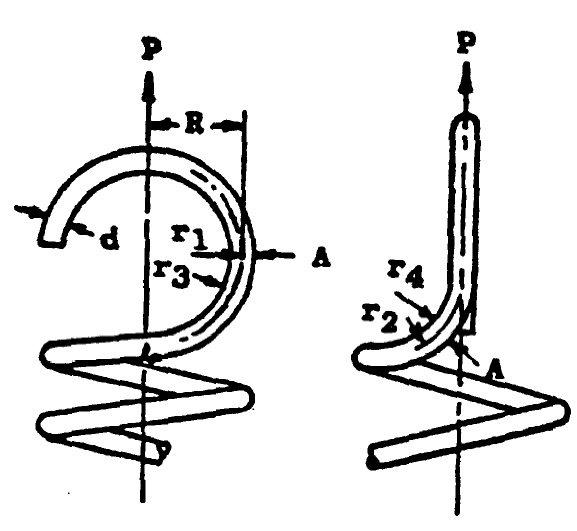
\includegraphics[width=0.8\textwidth]{milstd29a_fig43.png}
    \caption{}
    \label{fig:43}
\end{figure}

\begin{figure}[htbp] % h:here, t:top, b:bottom, p:page
    \centering
    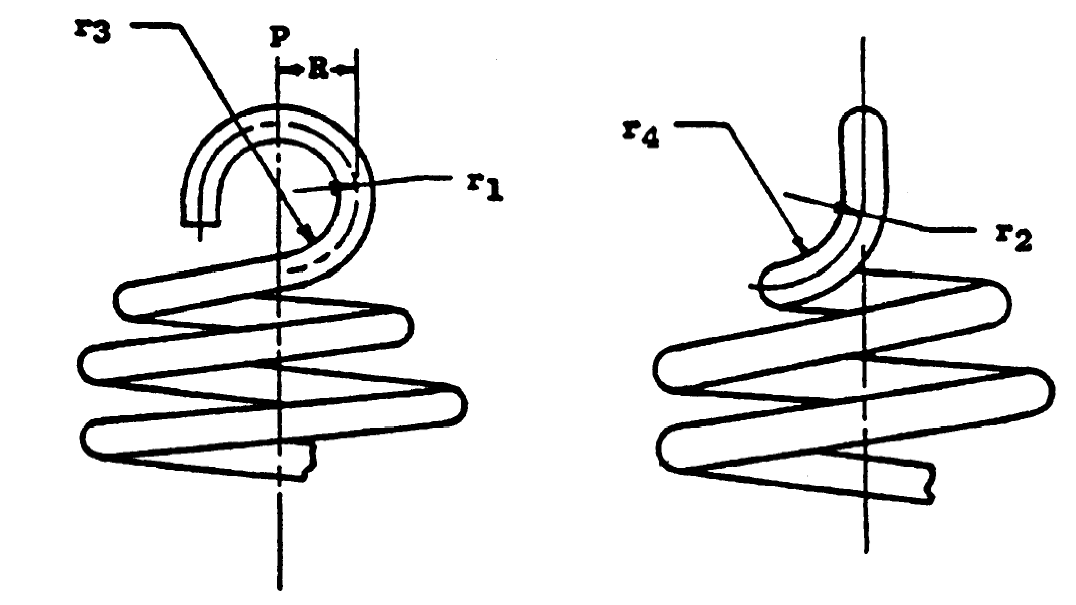
\includegraphics[width=0.8\textwidth]{milstd29a_fig44.png}
    \caption{}
    \label{fig:44}
\end{figure}

\subsection{Initial Tension} % Section 22.3
Initial tension is a load in pounds which opposes the opening of the coils by an external force. 
It is wound into the springs during the coiling operation.
Extension springs will have a unifom rate after the applied load overcomes the load due to initial tension. 
The number of coils do not affect the amount of initial tension except when the weight of the coils is heavier than the initial tension. 
The amount of initial tension is dependent on the spring index (D/d); the smaller the index the larger the initial tension. Initial tension does not increase the ultimate load or capacity of the spring but causes a larger portion thereof to be exerted during the initial deflection. 
For example, if the initial tension is 4 lbs and the spring rate is 9 lb then, at 1 inch deflection the load is

$$(1 \times 9) + 4 = 13 \mathrm{lb}$$

3-inches deflection the load is

$$(3 \times 9) + 4 = 31 \mathrm{lb}$$

In computing the total torsional stress add the torsional stress caused by initial tension to the torsional stress caused by deflection.
Figure 45 shows the amount of initial tension in terms of torsional stress (without application of curvature stress correction factor) which can be coiled into extension springs made of music wire, oil tempered, corrosion resisting steel and hard drawn spring steels.
Reduce these values 20 percent for springs made from nickel-base alloys such as Monel and Inconel. Hot rolled springs and those made of annealed materials cannot be wound with initial tension.
Springs which require stress relieving will lose 25 to 50 percent of their initial tension.
This loss can be compensated for during the coiling operation by winding more initial tension into the spring and thus obtain the required tension after stress relieving.

\subsection{Example of Extension Spring Calculation} % Section 22.4
An extension spring is required to exert a force (load)  of 27 lb at 2 in. defection and be deflected an additional 3 in. (5 in. total) and then exert a total load of 55 lb. 
It must operate within a 1.812 in. minimum diameter bore.

Select a suitable oil tempered wire diameter and determine the number of coils, length over coils, free length inside ends, maximum extended length inside ends without set, stresses at all loads, etc., stressed for light service (see Figure 62).

(yet to be transcribed)

\subsection{Precautions and Suggestions for Effective Design of Extension Springs} % Section 22.5
(a) Avoid using enlarged, extended, or specially shaped hooks or loops; they may double the cost of the spring and have high stress concentrations.

(b) If a plug must screw into the end of a spring, the spring should be coiled right hand.

(c) Nearly all extension springs are wound with enough initial tension to keep the spring together. Always figure on at least 5 to 10 percent of the final load as initial tension, unless otherwise specified.

(d) Electroplating does not deposit a good coating on the inside of, or between the coils of extension springs.

(e) Hooks on extension springs deflect under a load.
Each half hook, made by bending one-half of a coil, deflects an amount equivalent to 0.1 of an active coil.
Allowance for this deflection should be considered in design.

(f) If the relative position of the ends is not important note this fact on the drawing.

(g) For standard hooks keep the OD of the hook the same as the OD of the spring, and the distance from the end of the body, or from the last coil, to the inside of the hook about 75 to 85 percent of the ID of the spring.

(h) The body length or closed portion of an extension spring equals the number of coils in the body plus one, multiplied by the wire diameter.

(i) When deflected 1 1/4 times the maximum deflection as assembled, the total stress should be less than the Minimum Elastic Limit shown by the curves in Figure 62, as modified by their multiplying constants.

\subsection{Garter Springs} % Section 22.6
\subsubsection{General} % Section 22.6.1
Close coiled extension springs used in the form of rings by connecting the ends are often used as driving belts, for oil seals and as retainers.
The ends may have half or full loops and then be hooked together or one end may be reduced in diameter for three to six coils and screwed into the other end. 
Connecting the ends with a separate short section, called a connector, is occasionally done.

\subsection{Formulas}
(yet to be transcribed)

\subsection{Example of Calculation}
(yet to be transcribed)

\section{Torsion Springs} % Section 23.
\subsection{Design Formulas} % Section 23.1
(yet to be transcribed)

\subsection{Stresses in Torsion Spring Ends} % Section 23.2
(yet to be transcribed)

\subsection{Deflection of Torsion Spring Ends} % Section 23.3
(yet to be transcribed)

\subsection{Change in Diameter and Length} % Section 23.4
(yet to be transcribed)

\subsection{Helix} % Section 23.5
(yet to be transcribed)

\subsection{Design Nomographs for Helical Torsion Springs} % Section 23.6
(yet to be transcribed)

\subsection{Moment vs. Wire Size Chart} % Section 23.7
(yet to be transcribed)

\subsection{Torsion Spring Calculation} % Section 23.8
(yet to be transcribed)

\subsubsection{Example of Calculation} % Section 23.8.1
(yet to be transcribed)

\subsection{Precautions and Suggestions for Effective Design} % Section 23.9
(yet to be transcribed)

\section{Spiral Torsion Springs} % Section 24.
(yet to be transcribed)

\subsection{General}
(yet to be transcribed)

\subsection{Stress}
(yet to be transcribed)

\subsection{Ends}
(yet to be transcribed)

\section{Constant Force Springs}
\subsection{General}
(yet to be transcribed)
\subsection{Materials}
(yet to be transcribed)
\subsection{Inner Ends}
(yet to be transcribed)

\subsection{Outer Ends}
(yet to be transcribed)

\subsection{Multiple Mounting}
(yet to be transcribed)

\subsection{Stress Factor}
(yet to be transcribed)

\subsection{Extension Type}
(yet to be transcribed)

\subsection{Formulas}
(yet to be transcribed)

\subsection{Simplified Design}
(yet to be transcribed)

\subsection{Design Charts}
(yet to be transcribed)

\subsection{Example}
(yet to be transcribed)

\section{Flat Springs}
\subsection{Design}
(yet to be transcribed)

\subsection{Stress}
(yet to be transcribed)

\section{Coned Disc (Belleville) Springs}
\subsection{General}
(yet to be transcribed)

\subsection{Load Deflection}
(yet to be transcribed)

\subsection{Stress}
(yet to be transcribed)

\subsection{Loads}
(yet to be transcribed)

\section{Recommended Maximum Working Stresses}
\subsection{Fatigue Strength Curves}
(yet to be transcribed)

\subsubsection{Light Service}
(yet to be transcribed)

\subsubsection{Average Service}
(yet to be transcribed)

\subsubsection{Severe Service}
(yet to be transcribed)

\subsubsection{Other Materials}
(yet to be transcribed)

\subsection{Permissible Elevated Temperatures}
(yet to be transcribed)


\clearpage
% Page 58:
\setcounter{section}{29} % Sets the section counter
\section*{Appendix A, Section III}
\section{Spring Manufacture} % Section 30.
\subsection{General} % Section 30.1
Information on only a few operations is essential for design purposes.

\section{Stress Relieving} % Section 31.
The usual types of hardening and tempering ovens are used for stress relieving. 
Springs made from prehardened wire such as Music Wire, Oil Tempered, Hard Drawn, Corrosion Resisting 18-8 and similar materials are stress relieved by heating at low temperatures from 400 to 650$^{\circ}$ F. to reduce the residual stresses trapped in the wire during the coiling operation.
Springs made from annealed wire are hardened and tempered in a manner somewhat similar to tool steel. 
Precipitation hardening materials such as Beryllium-Copper, K-Monel, Inconel X, 17-7 PH and others are heated at varying temperatures, depending upon composition, for extended times from 1 hour to 16 hours.

\section{Cold Set to Solid} % Section 32.
This process is used to stabilize the free length of a compression spring, so that subsequent inadvertent or intentional compression to solid height will not change the loads at working deflections.

(a) If a compression spring is designed so that the elastic limit is not exceeded when the spring is compressed to solid height, no appreciable permanent set will occur, other than removal of small kinks in the wire. 
The note "Cold Set to Solid" should be specified on the drawing of such springs.

(b) If a spring is designed so that the elastic limit is exceeded when the spring is closed solid, permanent set will occur and the free length will be decreased.
Residual stresses of opposite sign will be set up in the wire when the load is released, so that if the spring again is closed solid it will withstand a higher calculated stress than the stress corresponding with the elastic limit.
If the initial free length of the spring is made greater than the calculated free length by the proper amount, overstressing the spring beyond the elastic limit by compressing it to solid height will stabilize the characteristics and produce the desired loads at working deflections. 
Additional cycles of compressing the spring to solid height and releasing the load will not further change the free length. 
However, there is a limit to this process. 
After a certain initial free length has been reached for a particular spring, the final free length after compression to a solid height will remain constant no matter what increases are made in initial free length.

(c) When a spring is designed so that the stress at solid height is so far above the elastic limit that the spring will not have the desired loads at the working deflections if cold
set to solid, the note "Shall compress to .....in. without permanent set" should be placed on the drawing. 
The computed stress at the specified length (equal to, or less than, the final assembled length) must be less than the stress at the elastic limit. 
Whenever practicable, this design of spring should be discarded in favor of a spring having a solid stress within limits that will permit closing solid without permanent set.

Several methods may be used to cold set to solid. 
Small air presses and foot presses can be used for light springs, power presses, and specifically built motorized equipment for larger springs, and hydraulic presses for
heavy springs. 
Light springs also may be compressed by hand over close fitting arbors.

\section{Grinding} % Section 33.
End coils of compression springs are ground whenever it is necessary for the springs 1. to stand upright, 2. to obtain a good seat against a contacting part, 3. to reduce buckling, and 4. to cause the springs to exert more uniform pressures under a diaphragm or against a mating part. 
This operation is expensive and should be avoided wherever it is practicable to do so especially on light springs with wire diameters under 1/32 inch and where a large spring index ratio (OD/d) prevails, such as 13 or larger.
Several types of disc grinding machines are available.
The small disc grinders using paddles to hold springs for grinding are especially useful for small production runs from 100 to 5000 or more springs.
Grinders with horizontal "ferris wheel" methods of loading are useful for larger quantities of light springs using wire diameters up to about 3/32 inch.
Heavier sizes may be ground in disc grinders with vertical ferris wheels.

\section{Shot Peening} % Section 34.
Spring life can be increased at least 30 per cent and has often been incressed from two to ten times by shot peening.
This process may be applied to all highly stressed springs made from steel and non-ferrous materials usually over 1/16 inch wire diameter.
Extension springs and closely wound torsion springs are difficult to shotpeen becasue the tiny steel shot if frequently trapped between the coils and is difficult to remove.
The large increase in fatigue life of helical springs due to shot peening is accomplished by a combination of effects:

(a) Small surface irregularities seen only by the microscope are hammered smooth.

(b) The surface of the wire is thoroughly cleaned, and sharp burrs are made dull.

(c) This additional cold work hardens the surface of the wire and raises the physical properties where the stress is the highest.

(d) Cold forging traps beneficial compression stresses near the wire surface which must be overcome by the destructive tensile stresses that cause fatigue failure before breakage can occur.
All heat treating of springs and all stress-relieving processes should be done prior to shot peening, except in those instances where electroplating is used; it is then necessary to reheat after plating.
Heating the springs above 500$^\circ$ F after shot peening counteracts much of the beneficial effects of the trapped compression stresses produced by shot peening.

Springs made from annealed, oil tempered or alloy steels that must be electroplated can be shot peened principally to clean the surface, thus avoiding the necessity of soaking them in acid solutions to remove scale.
The slightly roughened surface of shot peened springs does not produce a bright glossy, electroplated coating.

\section{Protective Coatings} % Section 35.
Uncoated or oil dipped springs are satisfactory where corrosive conditions are not a factor.
Black japanning is often used as it is a flexible, inexpensive finish suitable for many applications.
Enamels, lacquers and paint are occasionally used. 
Cadmium with supplementary chromate treatment provides one of the best electro deposited coatings because it is both flexible and corrosion resistant.

Nickel, chromium zinc and other metals are also deposited electrolytically.
Black oxide and phosphate coatings are occasionally specified.
Care must be used in applying coatings, first to use detergents, solvents, alkaline or vaporizing degreasers to remove oil and dirt, shotblasting or sand blasting to remove scale, and baking to remove the hydrogen embrittelement that may be caused by acid dipping or electroplating.

\section{Hydrogen Embrittlement} % Section 36.
Steel, particularly hardened steel, is susceptible to embrittlement resulting from hydrogen introduced by acid pickling, electroplating, or cathodic electrocleaning operations.
Absorbed hydrogen results in brittle behavior particularly under sustained loading in the presence of stress concentration.
Baking to relieve hydrogen embrittled springs should be accomplished by a method similar to that specified in specification QQ-Z-325 or QQ-P-416.

(a) Most hydrogen is evolved during acid pickling and can be reduced by using organic inhibitors in the solution.
The cleaning of springs by shotblasting or by tumbling is advisable so that less time is required in the picking bath.

(b)

(c)

(d)

(yet to be transcribed)


% Page 117:
% Table XIX:



% Page 118:
% Figure 63:
\begin{figure}[htbp] % h:here, t:top, b:bottom, p:page
    \centering
    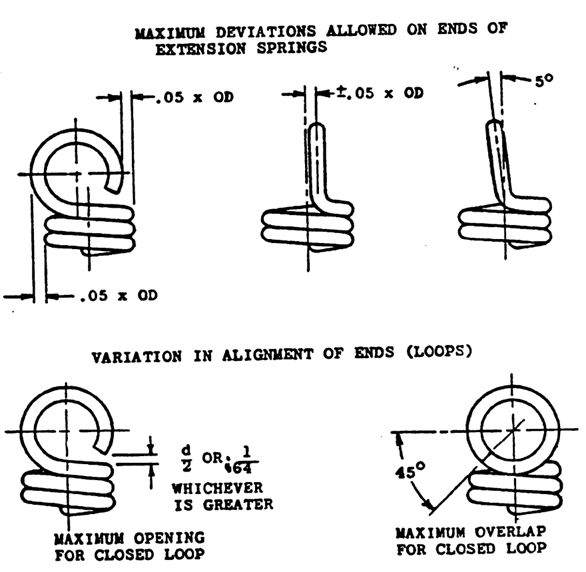
\includegraphics[width=0.8\textwidth]{milstd29a_fig63.png}
    \caption{Maximum Deviations Allowed on Ends of Extension Springs}
    \label{fig:63}
\end{figure}


% Page 119:
\section{Tolerances for Springs} % Section 37.
Tables that follow present tolerances which can be obtained under normal manufacturing methods. 
Springs having closer tolerances can be produced but at greatly increased cost.
A more liberal tolerance should be specified whenever possible.

% Table XX. Tolerances on squareness of grinding on end coils for compression springs:
\begin{table}[h!]
\centering
\caption{Tolerances on squareness of grinding on end coils for compression springs.}
\renewcommand{\arraystretch}{1.3}
\begin{tabularx}{\textwidth}{c|c|c|c}
\hline
\multirow{2}{*}{\parbox
{4cm}
{\centering Number of coils per inch of length (Number of coils ÷ length)}} 
& \multicolumn{3}{c}{Maximum tolerance from squareness to axis (degrees)} \\
\cline{2-4}
& \multicolumn{3}{c}{Spring Index (OD/d)} \\
\cline{2-4}
& Up to 6 (small) & 6 to 10 (average) & 10 to 16 (large) \\
\hline
Up to 7          & 3$^\circ$ & 4$^\circ$ & 5$^\circ$ \\
\hline
Over 7 to 12     & 4$^\circ$ & 5$^\circ$ & 6$^\circ$ \\
\hline
Over 12 to 17    & 5$^\circ$ & 6$^\circ$ & 7$^\circ$ \\
\hline
Over 17          & 6$^\circ$ & 7$^\circ$ & 8$^\circ$ \\
\hline
\end{tabularx}
\end{table}

These tolerances in degrees maybe reduced 50 per cent by individually grinding, measuring, testing, and sorting the springs, but this increases production time and cost.
Grinding end coils of springs made from wire under 1/32 inch diameter is usually unnecessary and frequently is expensive.

\subsection{Tolerance on Loads} % Section 37.1
The recommended tolerance on all loads is plus or minus 10 per cent and should be specified as shown on the drawing requirement charts. 
However, when the deflection from the free length to the limit load is small, the load tolerance must be large and should be considered proportional to the tolerances that apply to the free length. 
For example, if the deflection is only 1/8 inch and the tolerance on the free length is 1/32 inch, then it follows that the tolerance on the first load should be plus or minus 25 percent (1/32 = 25 percent of 1/8), otherwise the tolerance on the free length could not be taken.

Where a specific amount of initial tension is required for extension springs, it should be specified in pounds or ounces with a recommended tolerance of plus or minus 15 per cent, but it usually is specified as a REFERENCE.

Smaller load tolerances than these usually require testing and adjusting each spring and add considerably to the manufacturing time and to the cost.

Table XXI. Table of Third and Fourth Powers of Wire Diameters

Table XXII. Load changes due to slight wire changes

\clearpage
% Page 122:

Table XXIII. Causes of spring failure. Listed in sequence according to frequency of failure.

%\hrule

Spring failure may be cause by breakage, high permanent set or loss of load.
Group I lists the causes that occur most frequently.
Group II contains the less frequent causes and Group III lists causes that occur occasionally.

%\hrule

Group I:

HIGH STRESS

The majority of spring failures are due to high stresses caused by large deflections and high loads. 
High stresses should be used only for statically loaded springs. 
Low stresses lengthen fatigue life.

HYDROGEN EMBRITTLEMENT

Improper electro-plating methods and acid cleaning of springs, without proper baking treatment, cause spring steels to become brittle, and is a frequent cause of failure. 
Non-ferrous springs are immune.

SHARP BENDS \& HOLES

Sharp bends on extension, torsion and flat springs and holes or notches in flat springs cause high concentration of stress resulting in failure. 
Bend radii should be as large as possible, and tool marks avoided.

FATIGUE

Repeated deflections of springs, especially above 1,000,000 operations, even with medium stresses, may cause failure. 
Low stresses should be used for severe operating conditions.

Group II:

SHOCK LOADING

Impact, shock, and rapid loading cause far higher stresses than those computed by the regular spring formulas. 
High carbon spring steels do not withstand shock loading as well as alloy steels.

CORROSION

Slight rusting or pitting caused by acids, alkali, galvanic corrosion, stress corrosion cracking, or corrosive atmosphere weakens the material and causes higher stresses in the corroded area.

FAULTY HEAT TREATMENT

Keeping spring materials at the hardening temperature for longer periods than necessary causes an undesirable growth in grain structure resulting in brittleness even though the hardness may be correct.

FAULTY MATERIAL

Poor material containing inclusions, seams, slivers, and flat material with rough, slit or torn edges causes early failure.
Overdrawn wire, improper hardness, and poor grain structure also result in early failure.

Group III:

HIGH TEMPERATURE

High temperatures reduce spring temper (or hardness), lowers the modulus of elasticity thereby causing lower loads, reduces the elastic limit and increases corrosion. 
Corrosion resisting or nickel alloys should be used.

LOW TEMPERATURE

Temperatures below -40$^{\circ}$ F lessen the ability of carbon steels to withstand shock loads. Carbon steels become brittle at -70$^{\circ}$ F. 
Corrosion resisting, nickel or nonferrous alloys should be used.

FRICTION

Close fits on rods or in holes results in a wearing away of material and occasional failure.
The outside diameters of compression springs expand during deflection but they become smaller on torsion springs.

OTHER CAUSES

Enlarged hooks on extension springs increases the stress at the bends. 
Carrying too much electrical current will cause failure. 
Welding and soldering frequently destroy the spring temper. 
Tool marks, nicks, and cuts often became stress raisers. 
Deflecting torsion springs outwardly causes high stresses. 
Winding them tightly causes binding on supporting rods. 
High speed of deflection, vibration and surging due to operation near natural periods of vibration or their harmonics, cause increased stresses.

\begin{table}[h!]
\centering
\caption{Causes of spring failure. Listed in sequence according to frequency of failure.}
%\renewcommand{\arraystretch}{1.3}
%\begin{tabularx}{\textwidth}{|l|X|}
\begin{tabularx}{\textwidth}{|p{3cm}|p{12cm}|}
\hline
\multicolumn{2}{|l|}{\textbf{Spring failure may be caused by breakage, high permanent set, or loss of load. Group I lists the causes that occur most frequently. Group II contains the less frequent causes and Group III lists causes that occur occasionally.}} \\
\hline

\multicolumn{2}{|l|}{\textbf{GROUP I}} \\
\hline
\textbf{HIGH STRESS} &
The majority of spring failures are due to high stresses caused by large deflections and high loads. High stresses should be used only for statically loaded springs. Low stresses lengthen fatigue life. \\
\hline
\textbf{HYDROGEN EMBRITTLEMENT} &
Improper electro-plating methods and acid cleaning of springs, without proper baking treatment, cause spring steels to become brittle, and is a frequent cause of failure. Non-ferrous springs are immune. \\
\hline
\textbf{SHARP BENDS \& HOLES} &
Sharp bends on extension, torsion and flat springs and holes or notches in flat springs cause high concentration of stress resulting in failure. Bend radii should be as large as possible, and tool marks avoided. \\
\hline
\textbf{FATIGUE} &
Repeated deflections of springs, especially above 1{,}000{,}000 operations, even with medium stresses, may cause failure. Low stresses should be used for severe operating conditions. \\
\hline
\textbf{SHOCK LOADING} &
Impact, shock, and rapid loading cause far higher stresses than those computed by the regular spring formulas. High carbon spring steels do not withstand shock loading as well as alloy steels. \\
\hline

\multicolumn{2}{|l|}{\textbf{GROUP II}} \\
\hline
\textbf{CORROSION} &
Slight rusting or pitting caused by acids, alkali, galvanic corrosion, stress corrosion cracking, or corrosive atmosphere weakens the material and causes higher stresses in the corroded area. \\
\hline
\textbf{FAULTY HEAT TREATMENT} &
Keeping spring materials at the hardening temperature for longer periods than necessary causes an undesirable growth in grain structure resulting in brittleness even though the hardness may be correct. \\
\hline
\textbf{FAULTY MATERIAL} &
Poor material containing inclusions, seams, slivers, and flat material with rough, slit, or torn edges cause early failure. Overdrawn wire, improper hardness, and poor grain structure also result in early failure. \\
\hline

\multicolumn{2}{|l|}{\textbf{GROUP III}} \\
\hline
\textbf{HIGH TEMPERATURE} &
High temperatures reduce spring temper (or hardness), lower the modulus of elasticity thereby causing lower loads, reduce the elastic limit, and increase corrosion. Corrosion‑resisting or nickel alloys should be used. \\
\hline
\textbf{LOW TEMPERATURE} &
Temperatures below $-40^\circ$F lessen the ability of carbon steels to withstand shock loads. Carbon steels become brittle at $-70^\circ$F. Corrosion‑resisting, nickel, or non‑ferrous alloys should be used. \\
\hline
\textbf{FRICTION} &
Close fits on rods or in holes result in a wearing away of material and occasional failure. The outside diameters of compression springs expand during deflection but they become smaller on torsion springs. \\
\hline
\textbf{OTHER CAUSES} &
Enlarged hooks on extension springs increase the stress at the bends. Carrying too much electrical current will cause failure. Welding and soldering frequently destroy the spring temper. Tool marks, nicks, and cuts often become stress raisers. Deflecting torsion springs outwardly causes high stresses. Winding them tightly causes binding on supporting rods. High speed of deflection, vibration, and surging due to operation near natural periods of vibration or their harmonics cause increased stresses. \\
\hline

\end{tabularx}
\end{table}


% Page 123:
\clearpage
Copies of specification, standards, drawings, and publications required by contractors in connection with procurement functions should be obtained from the procuring activity or as directed by the contracting officer.

Copies of this standard for military use may be obtained as indicated in the foreword to or general provisions of the Index of Military Specifications and Standards.

Copies of this Standard may be obtained for other than official use by individuals, firms, and contractors from the Superintendent of Documents, U. S. Government Printing Office, Washington 25. D. C.

Both the title and the identifying symbol number should be stipulated when requesting copies of Military Standards.

Patent notice. 
When Government drawings, specifications, or other data are used for any purpose other than in connection with a definitely related Government procurement operation, the United States Government thereby incurs no responsibility, nor any obligation whatsoever; and the fact that the Government may have formulated, furnished or in any way supplied the said drawings, specifications, or other data is not to be regarded by implication or otherwise as in any manner licensing the holder or any other person or corporation, or conveying any rights or permission to manufacture, use, or sell any patented invention that may in any way be related thereto.

\noindent Custodians:

Army - Ordnance Corps

Navy - Bureau of Naval Weapons

Air Force

\noindent Preparing activity:

Navy - Bureau of Naval Weapons


\end{document}